\documentclass[12pt]{report}

\usepackage{tikz}
\usepackage{eqparbox}
\usepackage{mathtools}
\usepackage{amsmath}
\usepackage{amsfonts}
\usepackage{systeme}
\usepackage{siunitx}
\usepackage[T1]{fontenc}
\usepackage{hyperref}
\usepackage{bigfoot}
\usepackage[numbered, framed]{matlab-prettifier}
\usepackage{filecontents}
\usepackage{graphicx}
\usepackage{pdfpages}
\hypersetup{
colorlinks,
citecolor=black,
filecolor=black,
linkcolor=black,
urlcolor=black
linkto=all,
}

\usetikzlibrary{automata, shapes.geometric, arrows.meta, calc, matrix, positioning}

\tikzstyle{startstop} = [rectangle, text width=5cm, rounded corners, minimum width=3cm, minimum height=1cm,text centered, draw=black]
\tikzstyle{io} = [trapezium, text width=3cm, trapezium left angle=70, trapezium right angle=110, minimum width=3cm, minimum height=1cm, text centered, draw=black]
\tikzstyle{arrow} = [thick,->,>=stealth]

\newenvironment{simplechar}{%
   \catcode`\^=12
}{}

\title{Numerical Methods, project C, Number 32}
\author{Krzysztof Rudnicki\\ Student number: 307585 \\ Advisor: dr hab. Piotr Marusak}
\date{\today}

\let\ph\mlplaceholder % shorter macro
\lstMakeShortInline"

\lstset{
  style              = Matlab-editor,
  basicstyle         = \mlttfamily,
  escapechar         = ",
  mlshowsectionrules = true,
}

\newcommand\myeq{\mathrel{\overset{\makebox[0pt]{\mbox{\normalfont\tiny\sffamily def}}}{=}}}


\begin{document}
\maketitle
\tableofcontents

\chapter{Determine polynomial function fitting experimental data}
\section{Problem}
Given following samples:
\begin{center}
  \begin{tabular}{| c | c |}
\hline
$x_i$ & $y_i$ \\
\hline
-5 & -6.5743\\
\hline
-4 & 0.9765\\
\hline
-3 & 3.1026\\
\hline
-2 & 1.8572 \\
\hline
-1 & 1.3165 \\
\hline
0 & -0.6144 \\
\hline
1 & 0.1032 \\
\hline
2 & 0.3729 \\
\hline
3 & 2.5327 \\
\hline
4 & 7.3857 \\
\hline
5 & 9.4892 \\
\hline

\end{tabular}
\end{center}

We have to determine polynomial function $ y  = f(x) $ that best fits this data. \\
We will use least-square approximation using system of normal equation with QR factorization.

\section{Theoretical introduction}
\subsection{Linear Least Squares Problem}
We have polynomial function:
\[ y(x) = a_nx^n + a_{n-1}x^{n-1} + \dots + a_1x^1 + a_0 \]
where n - degree of the polynomial we use to approximate function \\
Given matrix $\mathbf{A} \in \mathbb{R}^{m \times n} \quad (m > n)$ and vector $\mathbf{y} \in \mathbb{R}^m$ \\
We need to find vector \^{x} such that:
\[ 	\forall x \in \mathbb{R}^n \quad|| \mathbf{y} - \mathbf{A} \hat{x} ||_2 \leq || \mathbf{y} - \mathbf{A}x ||_2  \]
$\mathbf{A}\hat{x}$ is the vector of values of the approximating function at each data point and $y$ is the vector of values of data points. \\
We have to minimize the Euclidean norm of difference between approximation and data points. \\
To obtain $\hat{x}$ we will calculate the derrivative of error function with respect to $b_n$ and equate it to 0. This way we will get system of equations caled \textbf{normal equations} which have unique solution in form of vector $\hat{x}$

\subsection{Gram matrix and QR decomposition}
We will use Gram's matrix since it's condition number tends to be pretty high which improves the accuracy of our solution. \\
Gram's matrix is a matrix of set of normal equations. The simplest way to present normal equations is by using formula:
\[ \langle \phi_i, \phi_k \rangle \myeq \sum_{j=0}^N \phi_i(x_j)fi_k(x_j) \]
Which then leads to following matrix \textbf{A}:

\[
A = \begin{bmatrix}
\phi_0(x_0) & \phi_1(x_0) &  \dots & \phi_n(x_0) \\
\phi_0(x_1) & \phi_1(x_1) & \dots & \phi_n(x_1) \\
\phi_0(x_2) & \phi_1(x_2) & \dots & \phi_n(x_2) \\
\vdots & \vdots & \vdots & \vdots \\
\phi_0(x_N) & \phi_1(x_N) & \dots & \phi_n(x_N) \\
\end{bmatrix}
\]

In our case we define matrix \textbf{A} as:
\[
A = \begin{bmatrix}
1 & x_0 & (x_0)^2  & \dots & (x_0)^n \\
1 & x_1 & (x_1)^2 &  \dots & (x_1)^n\\
1 & x_2 & (x_2)^2 &  \dots & (x_2)^n\\
\vdots & \vdots & \vdots & \vdots \\
1 & x_N & (x_N)^2 &  \dots & (x_N)^n\\
\end{bmatrix}
\]

Where $x_N$ is the x-axis position for the N-th data point. Then we can express system of natural equations using A in this way:
\[ A^Ty = (A^TA)\hat{x} \]

With condition number of A equal to square root of condition number of Gram's matrix which gives us small errors. It is also usefull for QR factoization since we can rewrite it as follows:
\[ (R^TQ^T)(QR)\hat{x} = (R^TQ^T)y \]
Since determinant of $R \neq 0$ and $Q^TQ = I$ we can simplify aforementioned equation to:
\[ R\hat{x} = Q^Ty \]
And to optimize even further ahead insetead of using QR decomposition we can use faster $\tilde{Q}\tilde{R}$ decomposition:
\[ \tilde{R}\hat{x} = (\tilde{Q}^T\tilde{Q})^{-1}(\tilde{Q}^T) \]
This is faster since $\tilde{R}$ is an upper triangular matrix, easily solved using back-substitution.

\subsection{Gram-Schmidt algorithm}
We will use Gram-Schmidt algorithm for $\tilde{Q}\tilde{R}$ decomposition.
Gram-Schmidt algorithm takes non-orthogonal function basis denoted as:
\[ \phi_0, \dots, \phi_n \]
and orthogonalizes it into orthogonal function basis denoted as:
\[ \psi_0, \dots, \psi_n \]
Standard Gram-Schmid algorithm looks like this:
\[ \psi_0 = \phi_0 \]
\[ \psi_1 = \phi_1 - \frac{\langle \psi_0, \phi_1 \rangle}{\langle \psi_0, \psi_0 \rangle} \psi_0 \]
\[ \psi_n = \phi_n - \sum_{j = 0}^{i-1}  \frac{\langle \psi_j, \phi_i \rangle}{\langle \psi_j, \psi_j \rangle} \psi_j \]
Where $ i = 2, \dots, n $
Then we get a very well conditioned set of normal equations:
\[ a_0\langle \psi_0, \psi_0 \rangle = \langle f, \psi_0 \rangle \]
\[ a_1\langle \psi_1, \psi_1 \rangle = \langle f, \psi_1 \rangle \]
\[ \vdots \]
\[ a_n\langle \psi_n, \psi_n \rangle = \langle f, \psi_n \rangle \]

\section{Results}

I decided to simulate polynomials up to $\mathbf{10^{th}}$ degree.

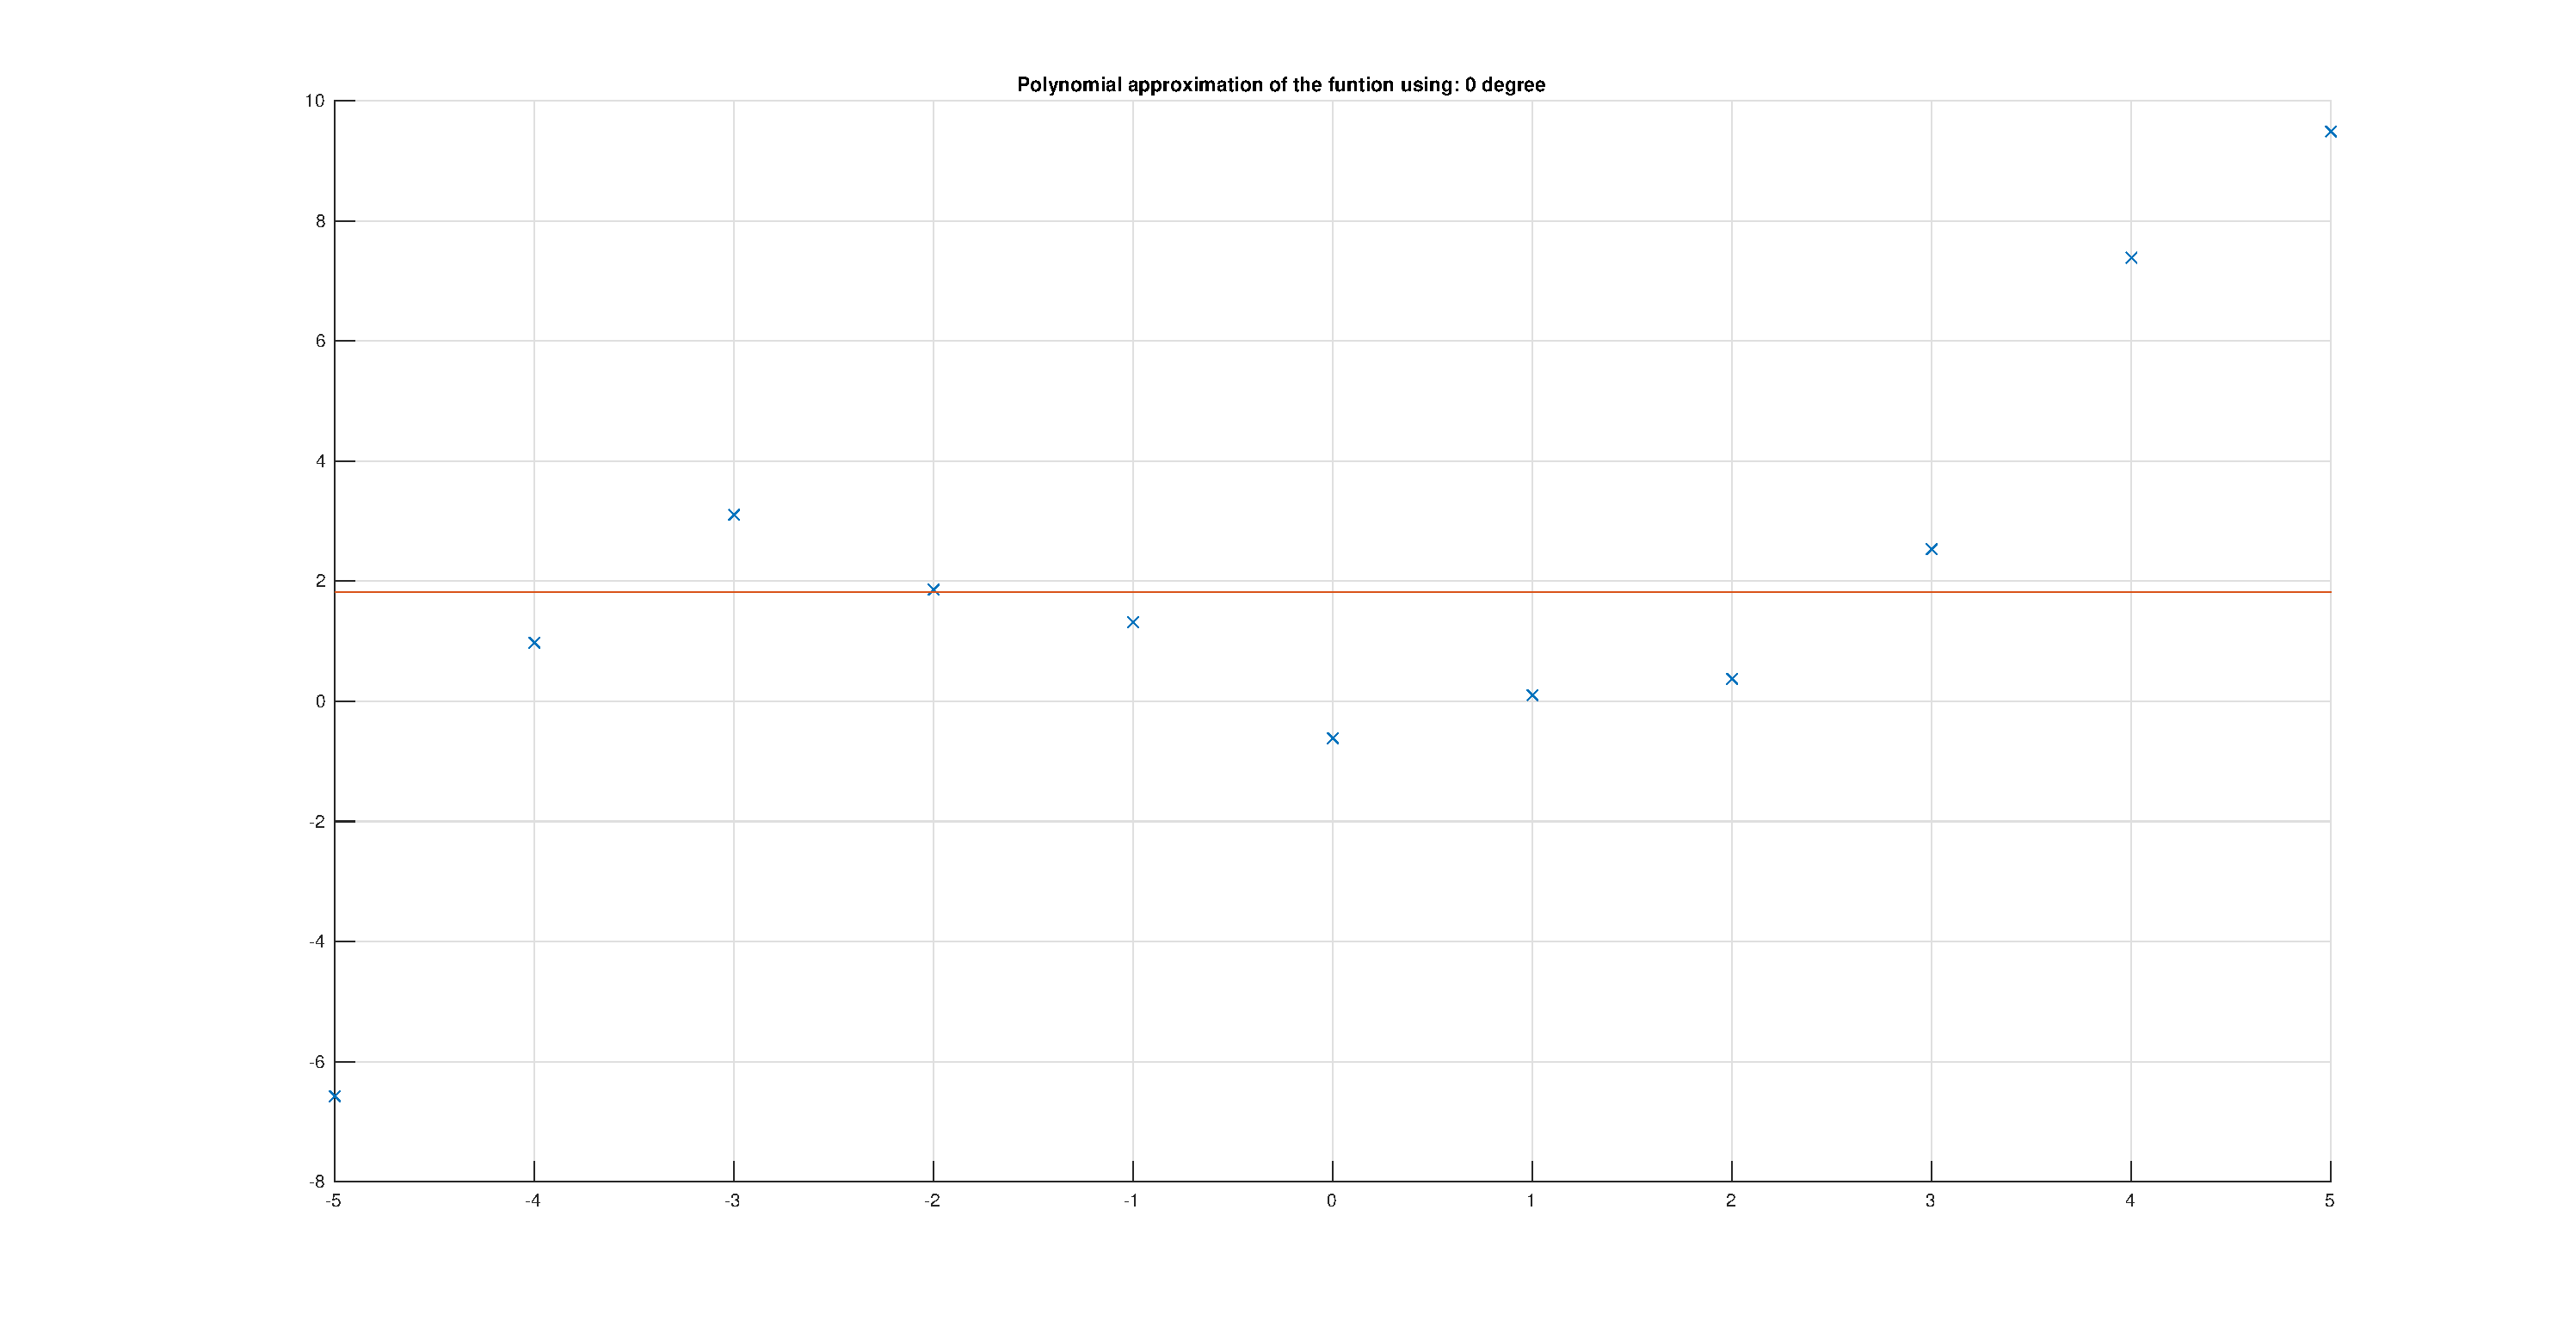
\includepdf[pages=-]{10-eps-converted-to.pdf}
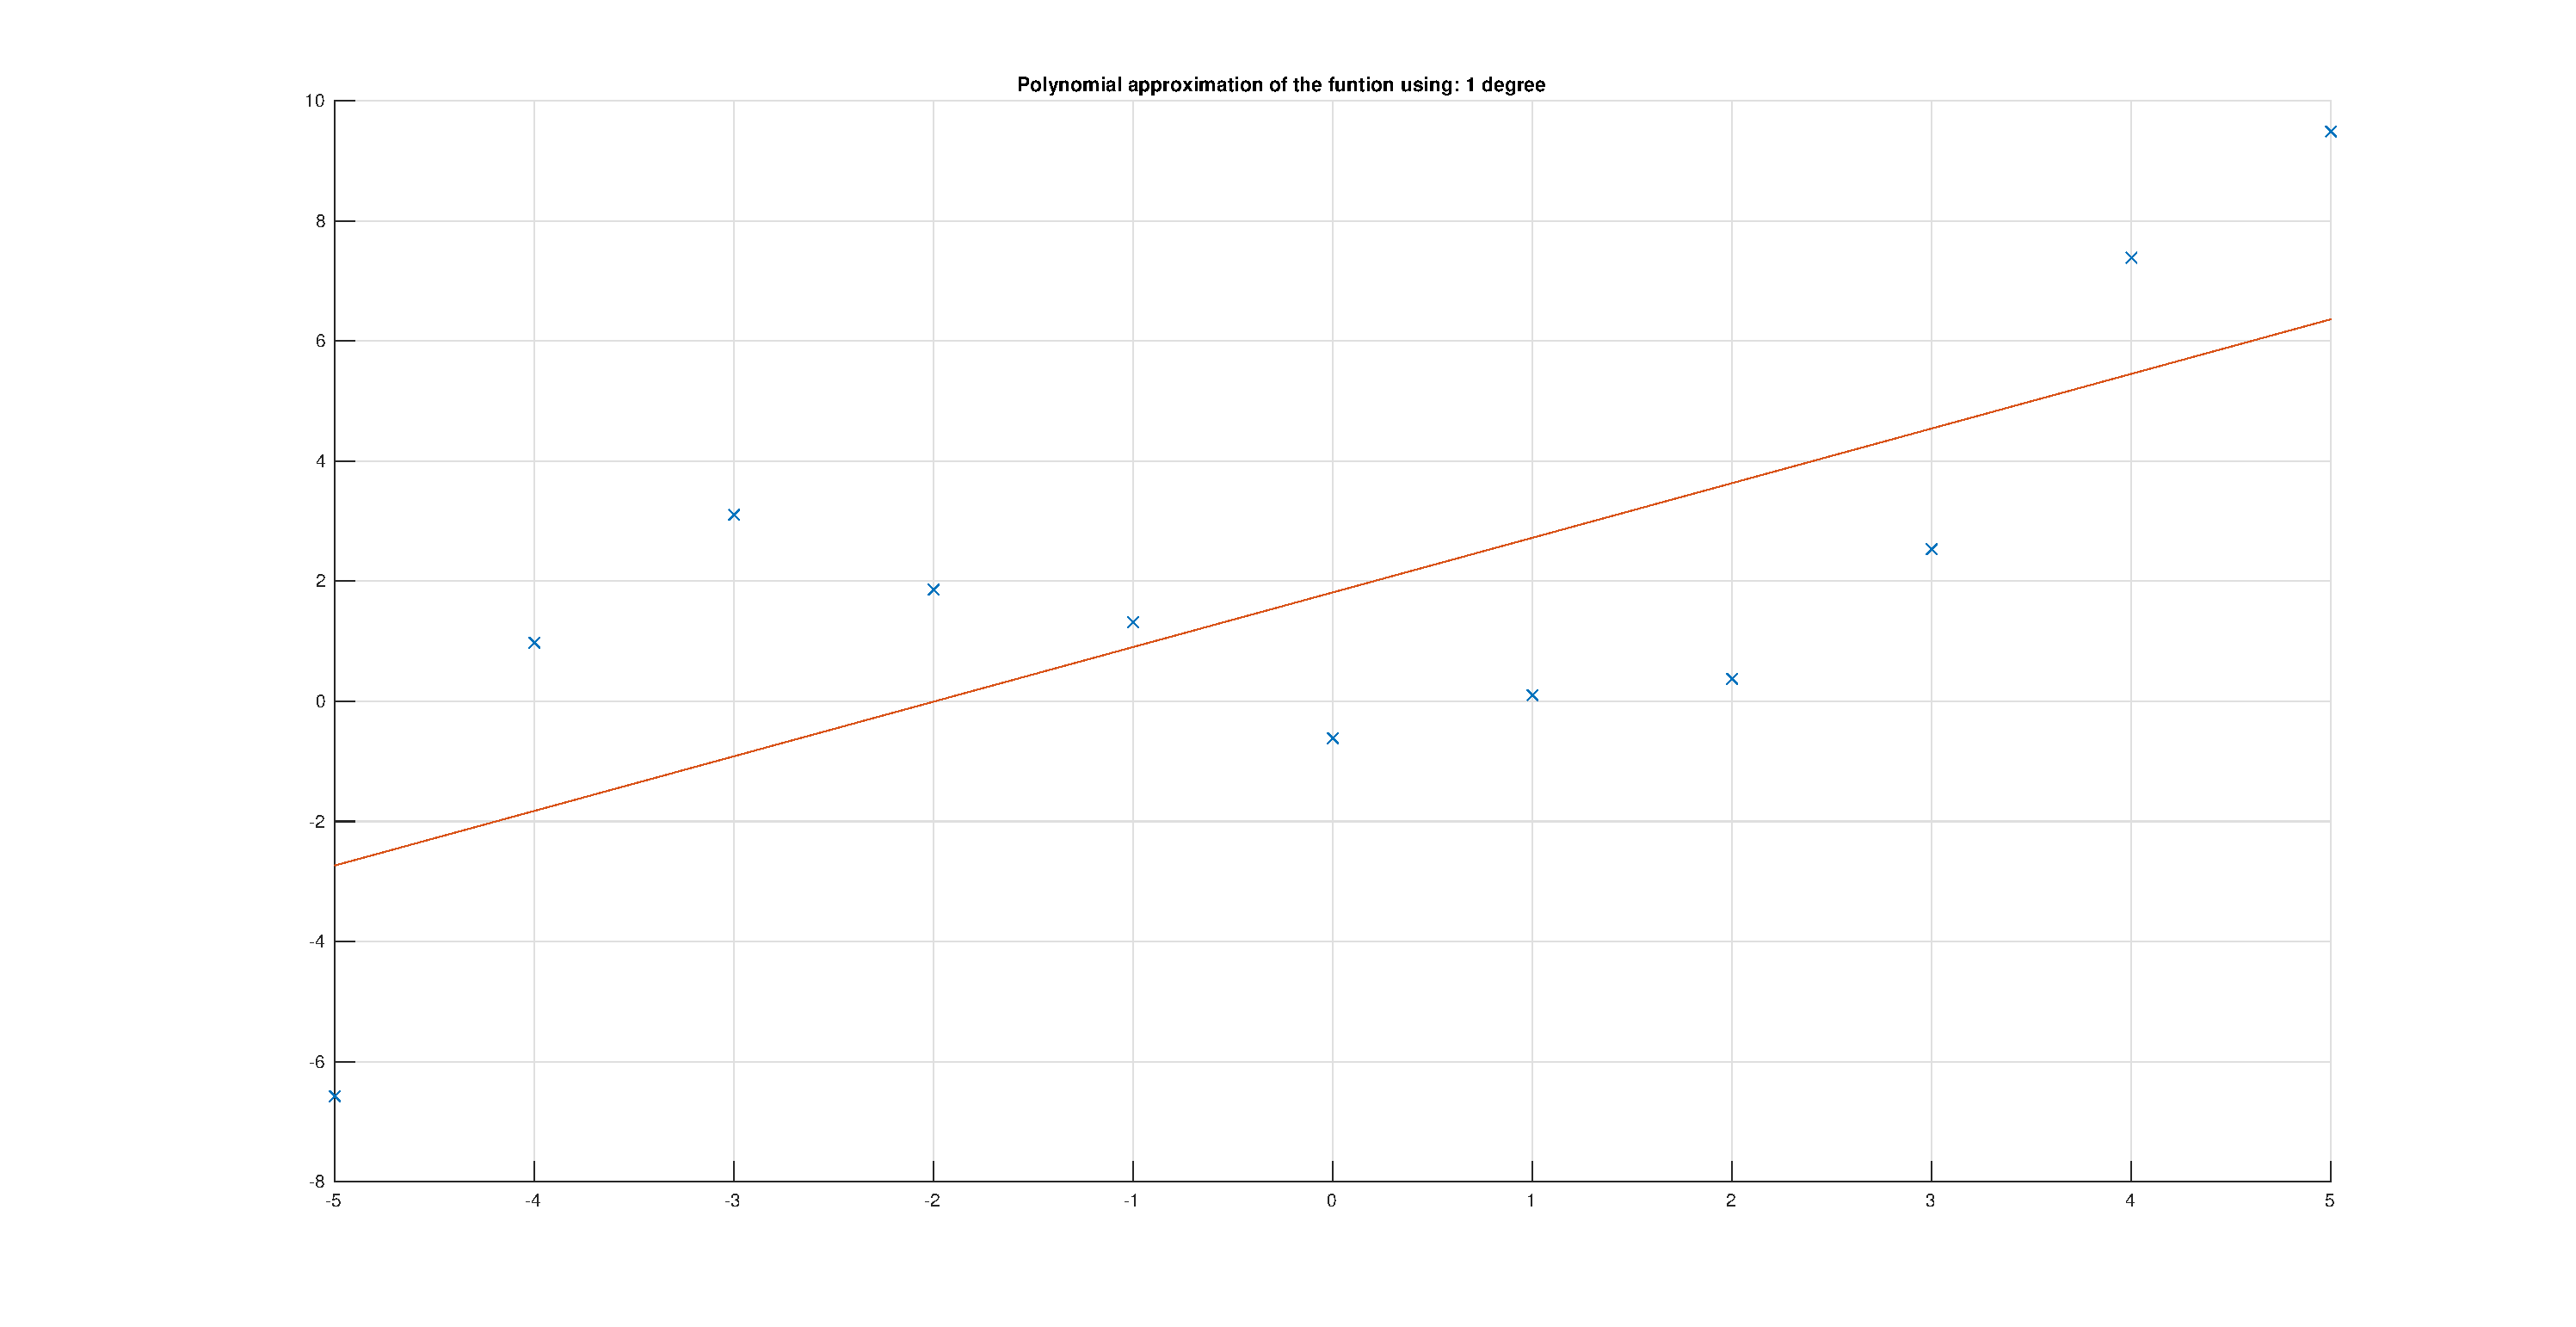
\includepdf[pages=-]{11-eps-converted-to.pdf}
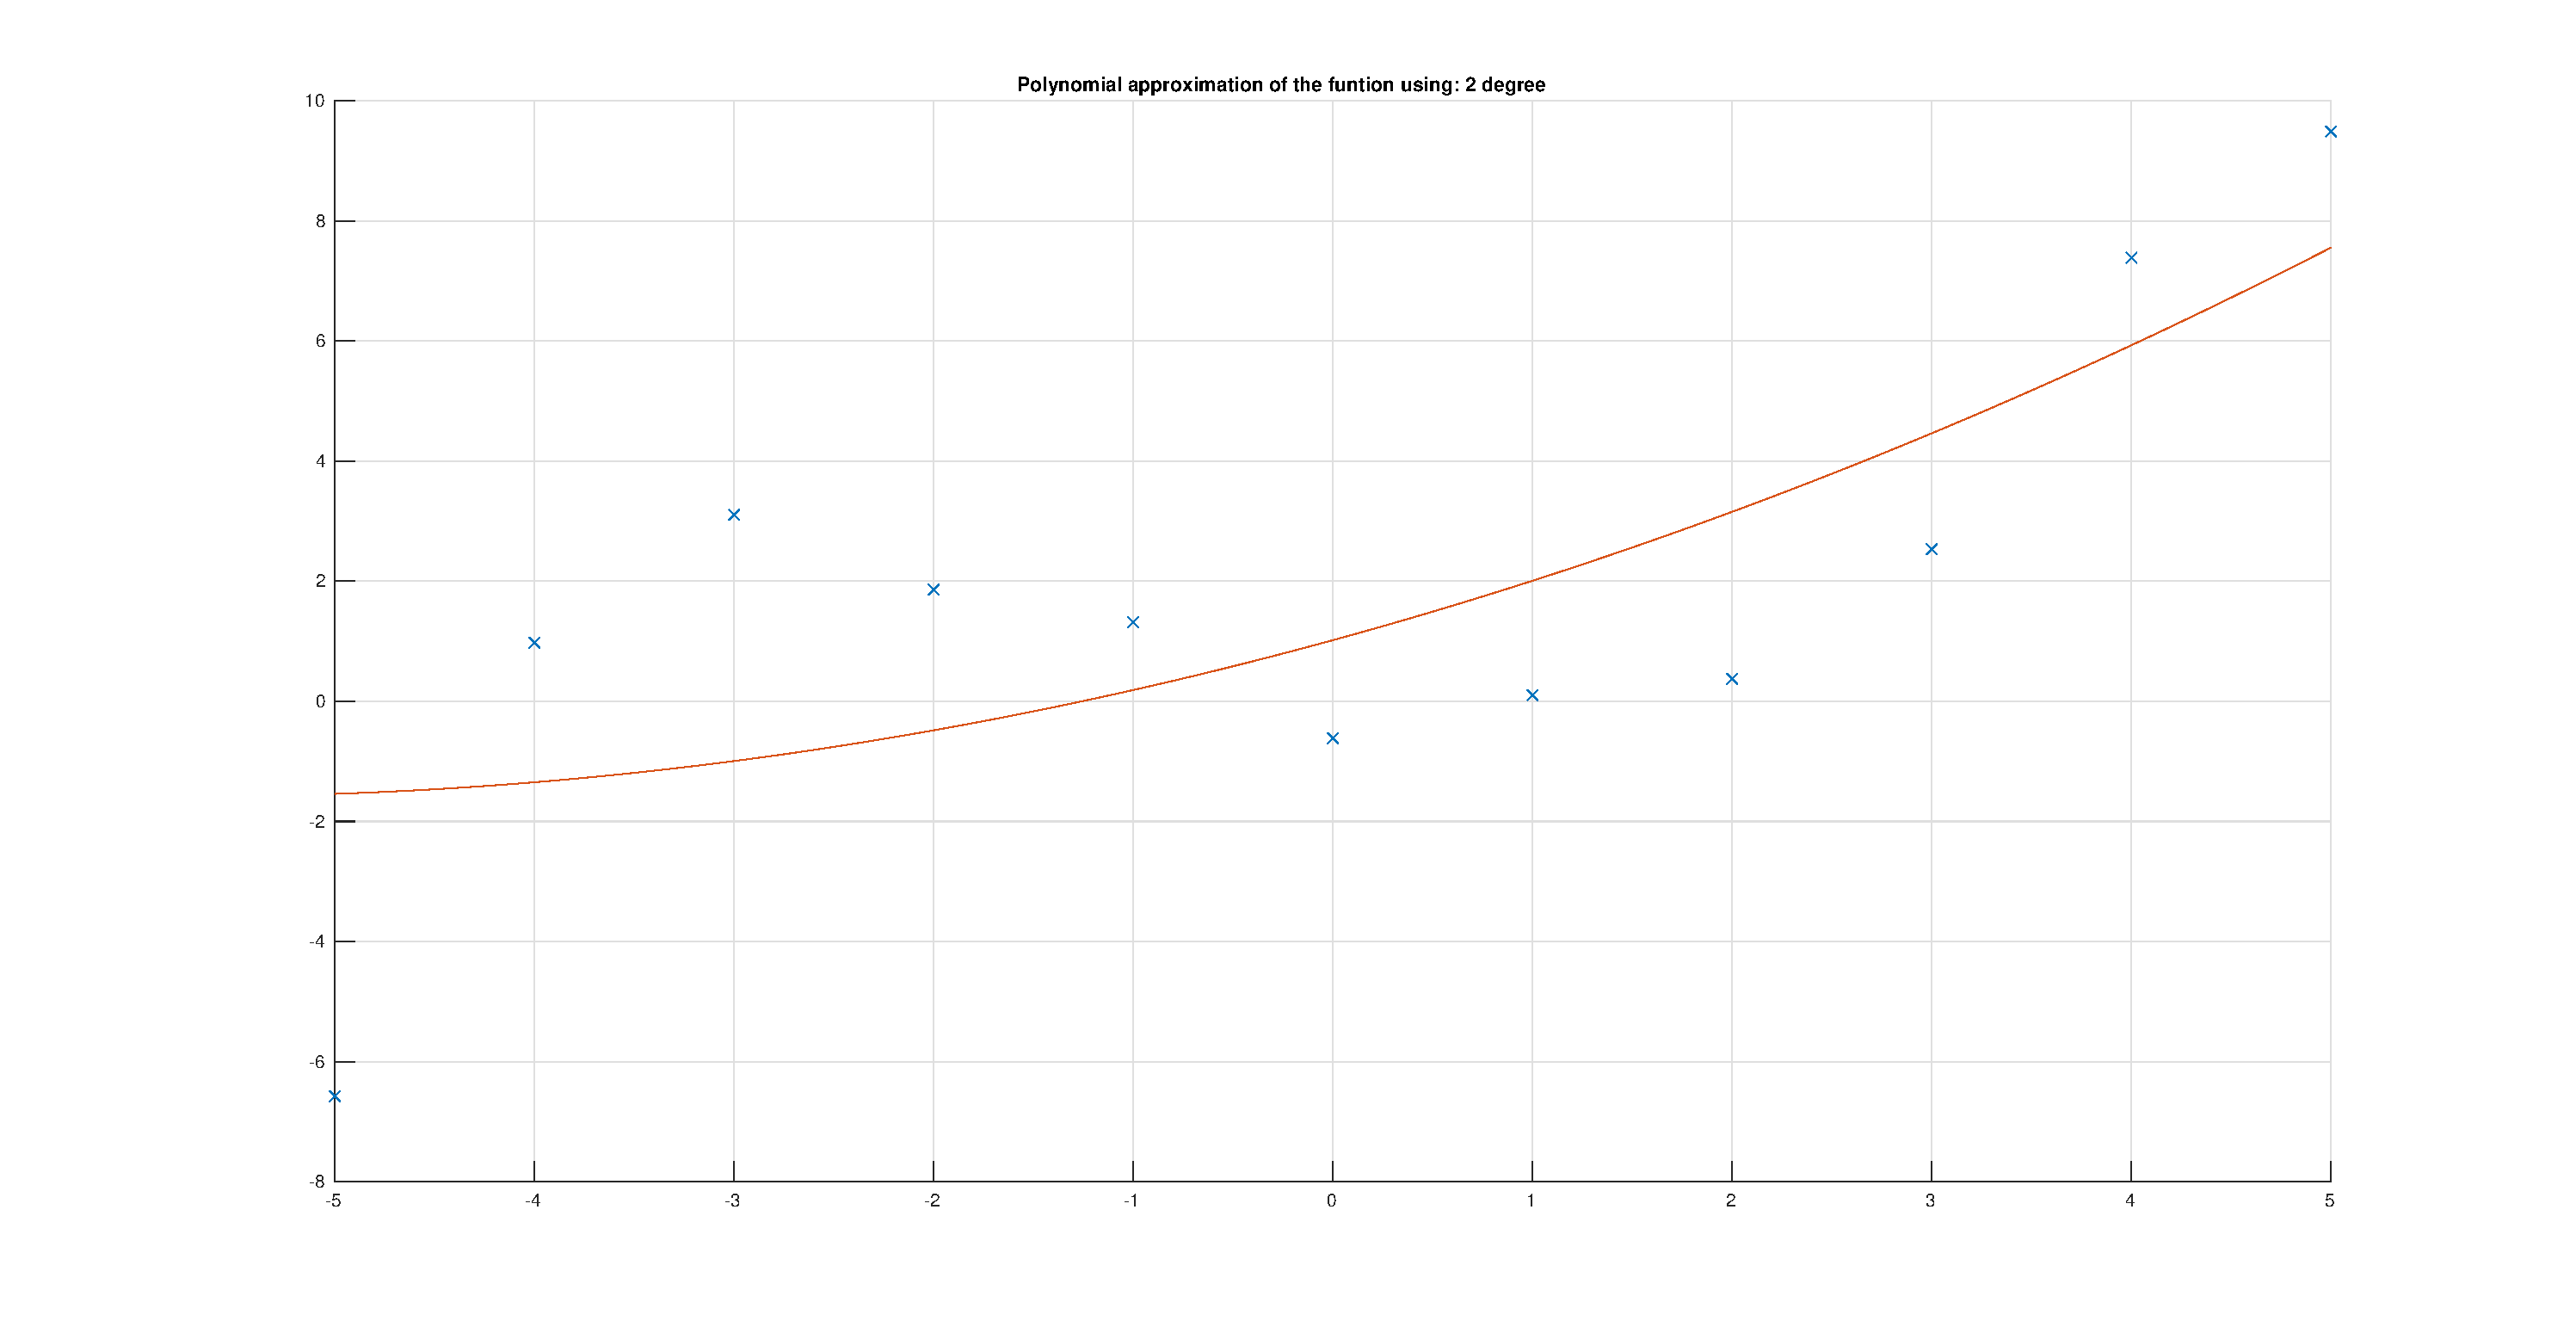
\includepdf[pages=-]{12-eps-converted-to.pdf}
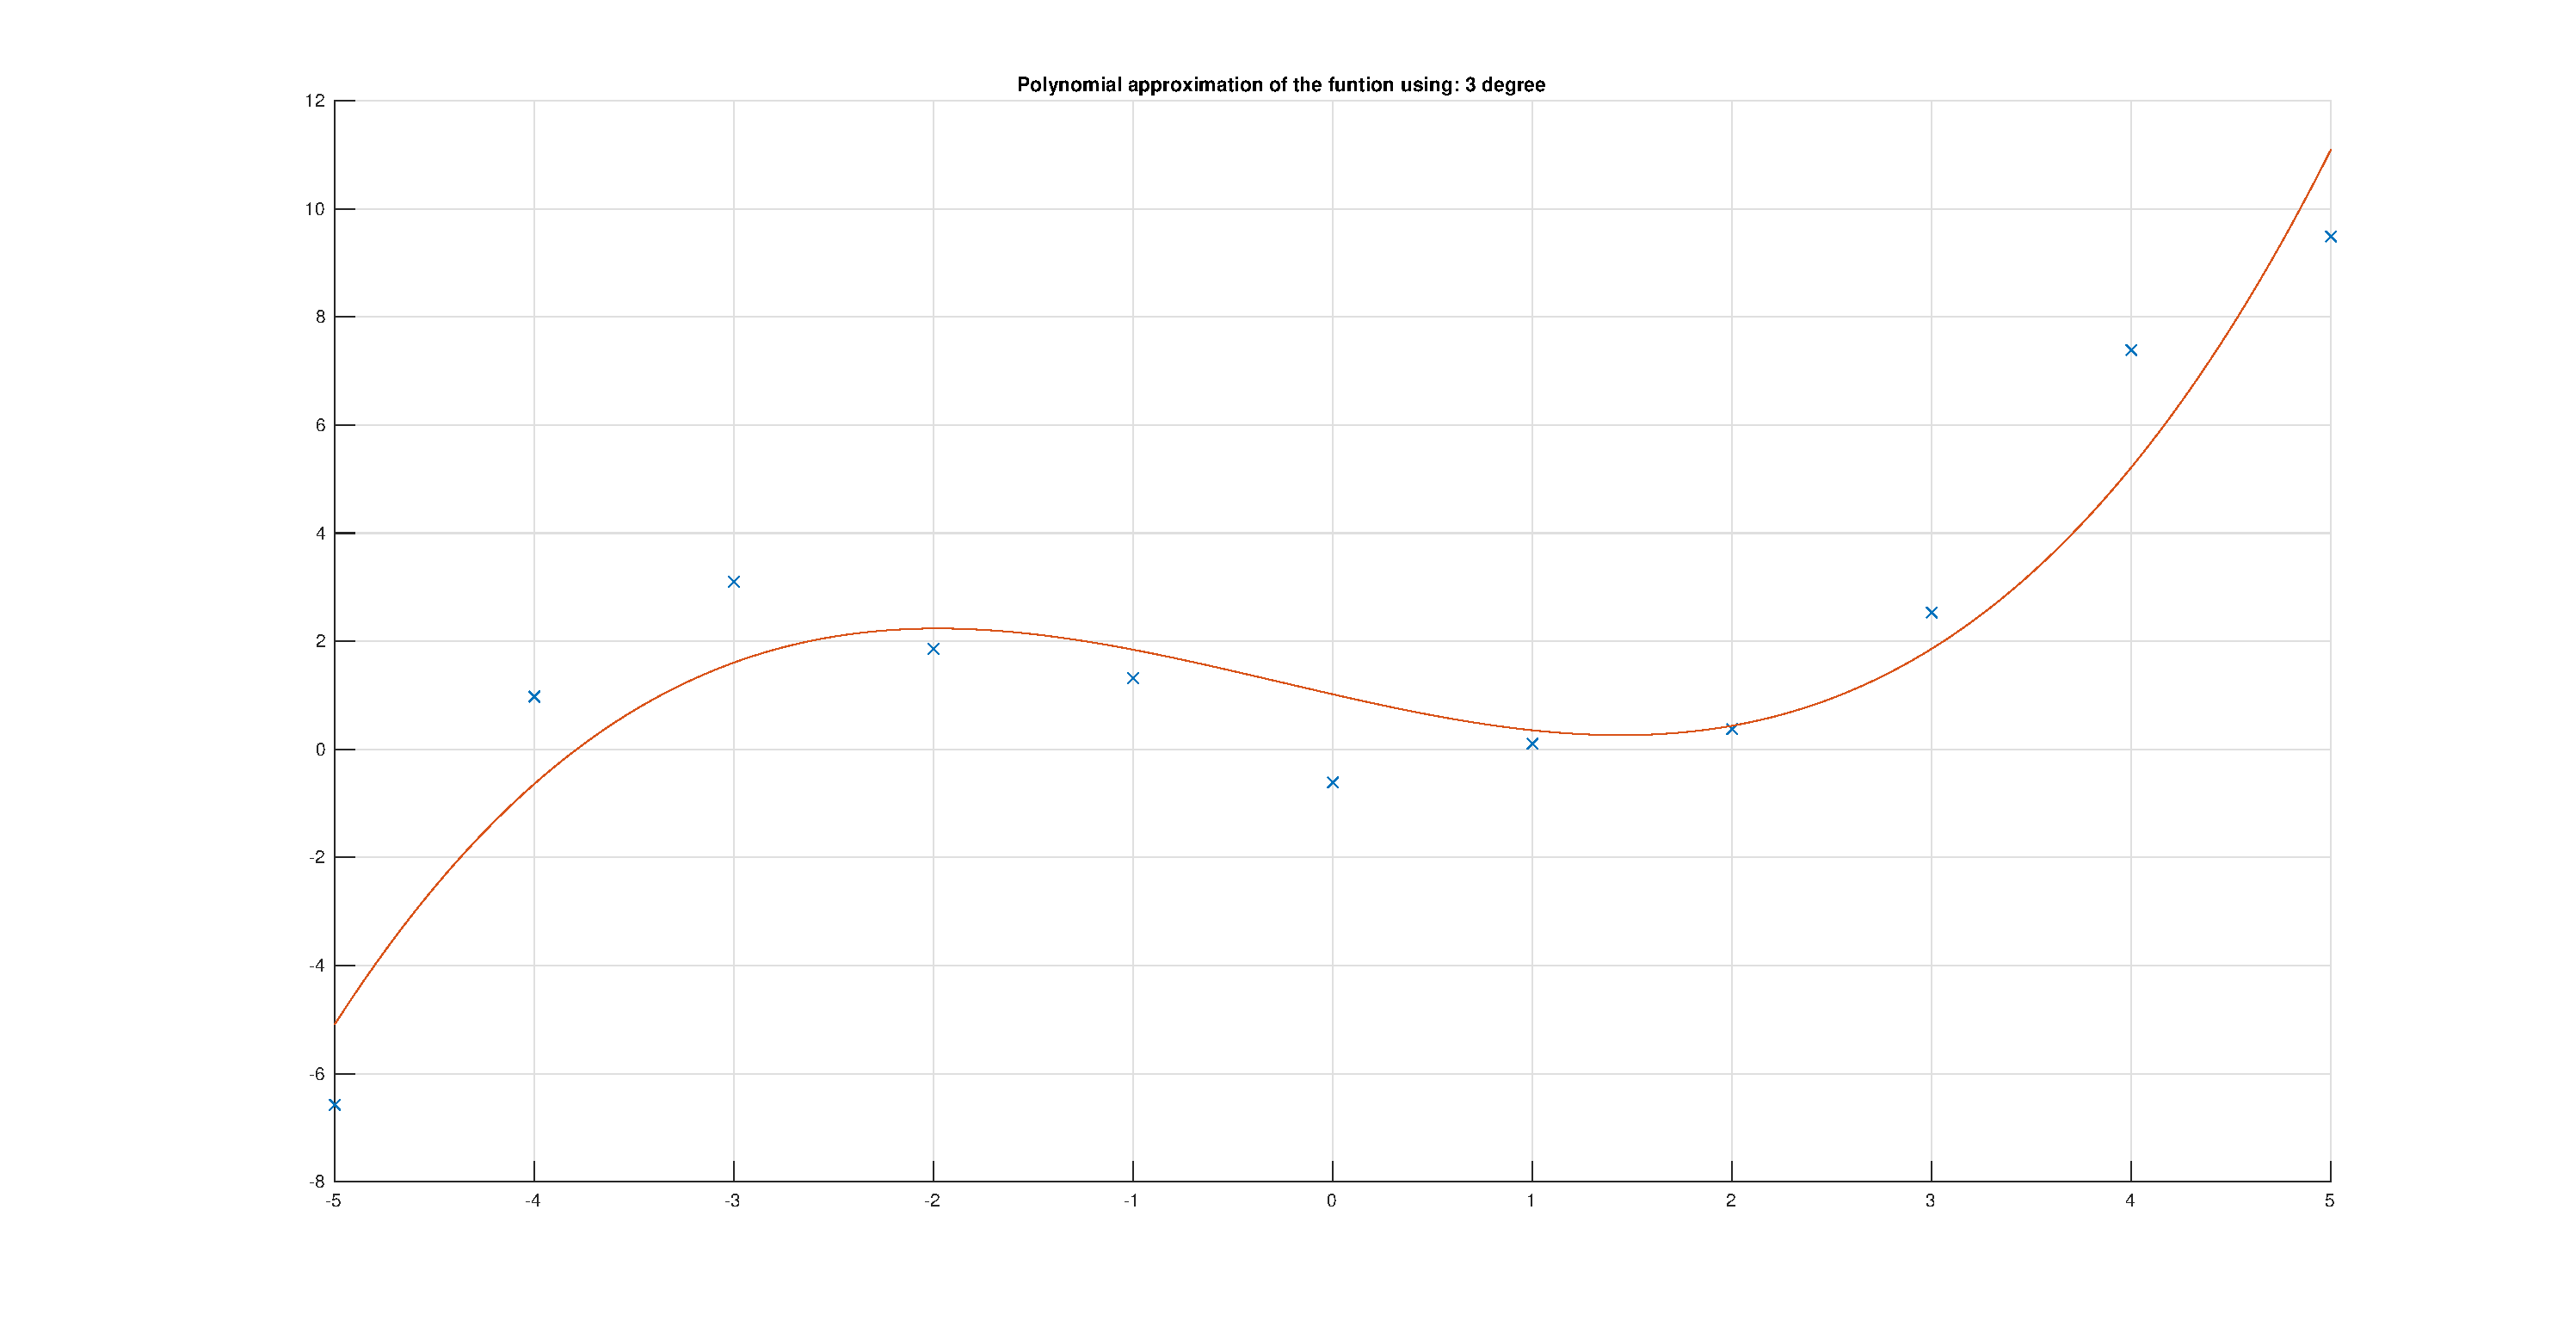
\includepdf[pages=-]{13-eps-converted-to.pdf}
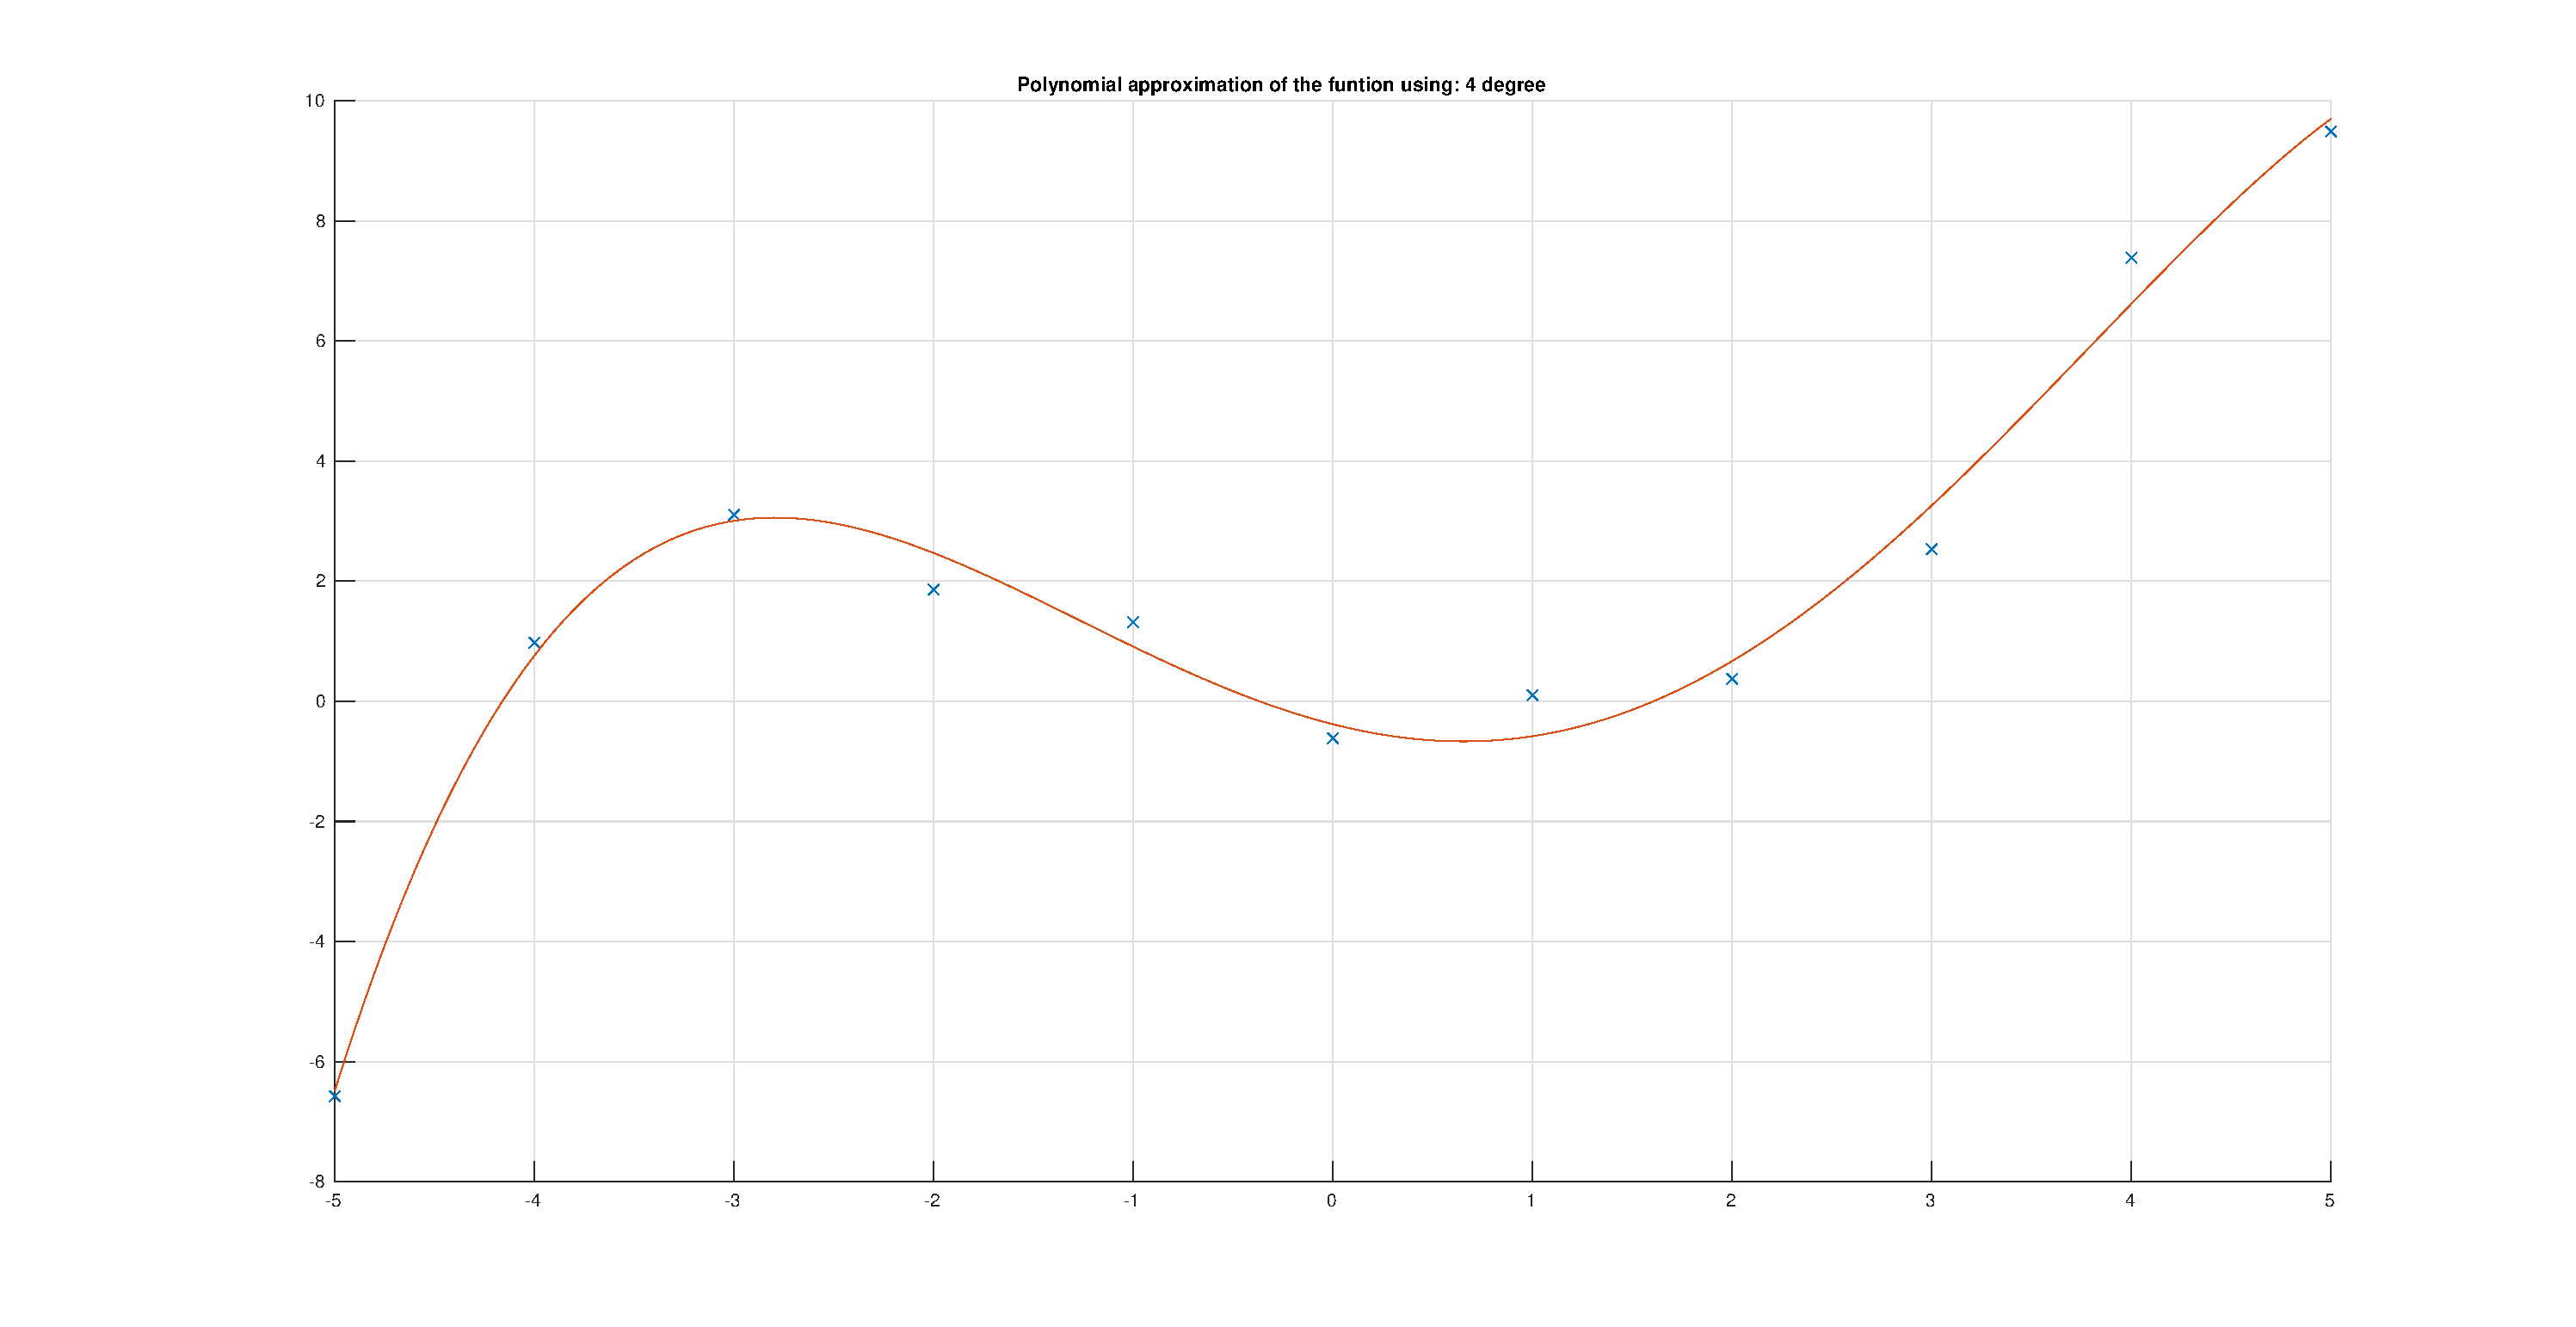
\includepdf[pages=-]{14-eps-converted-to.pdf}
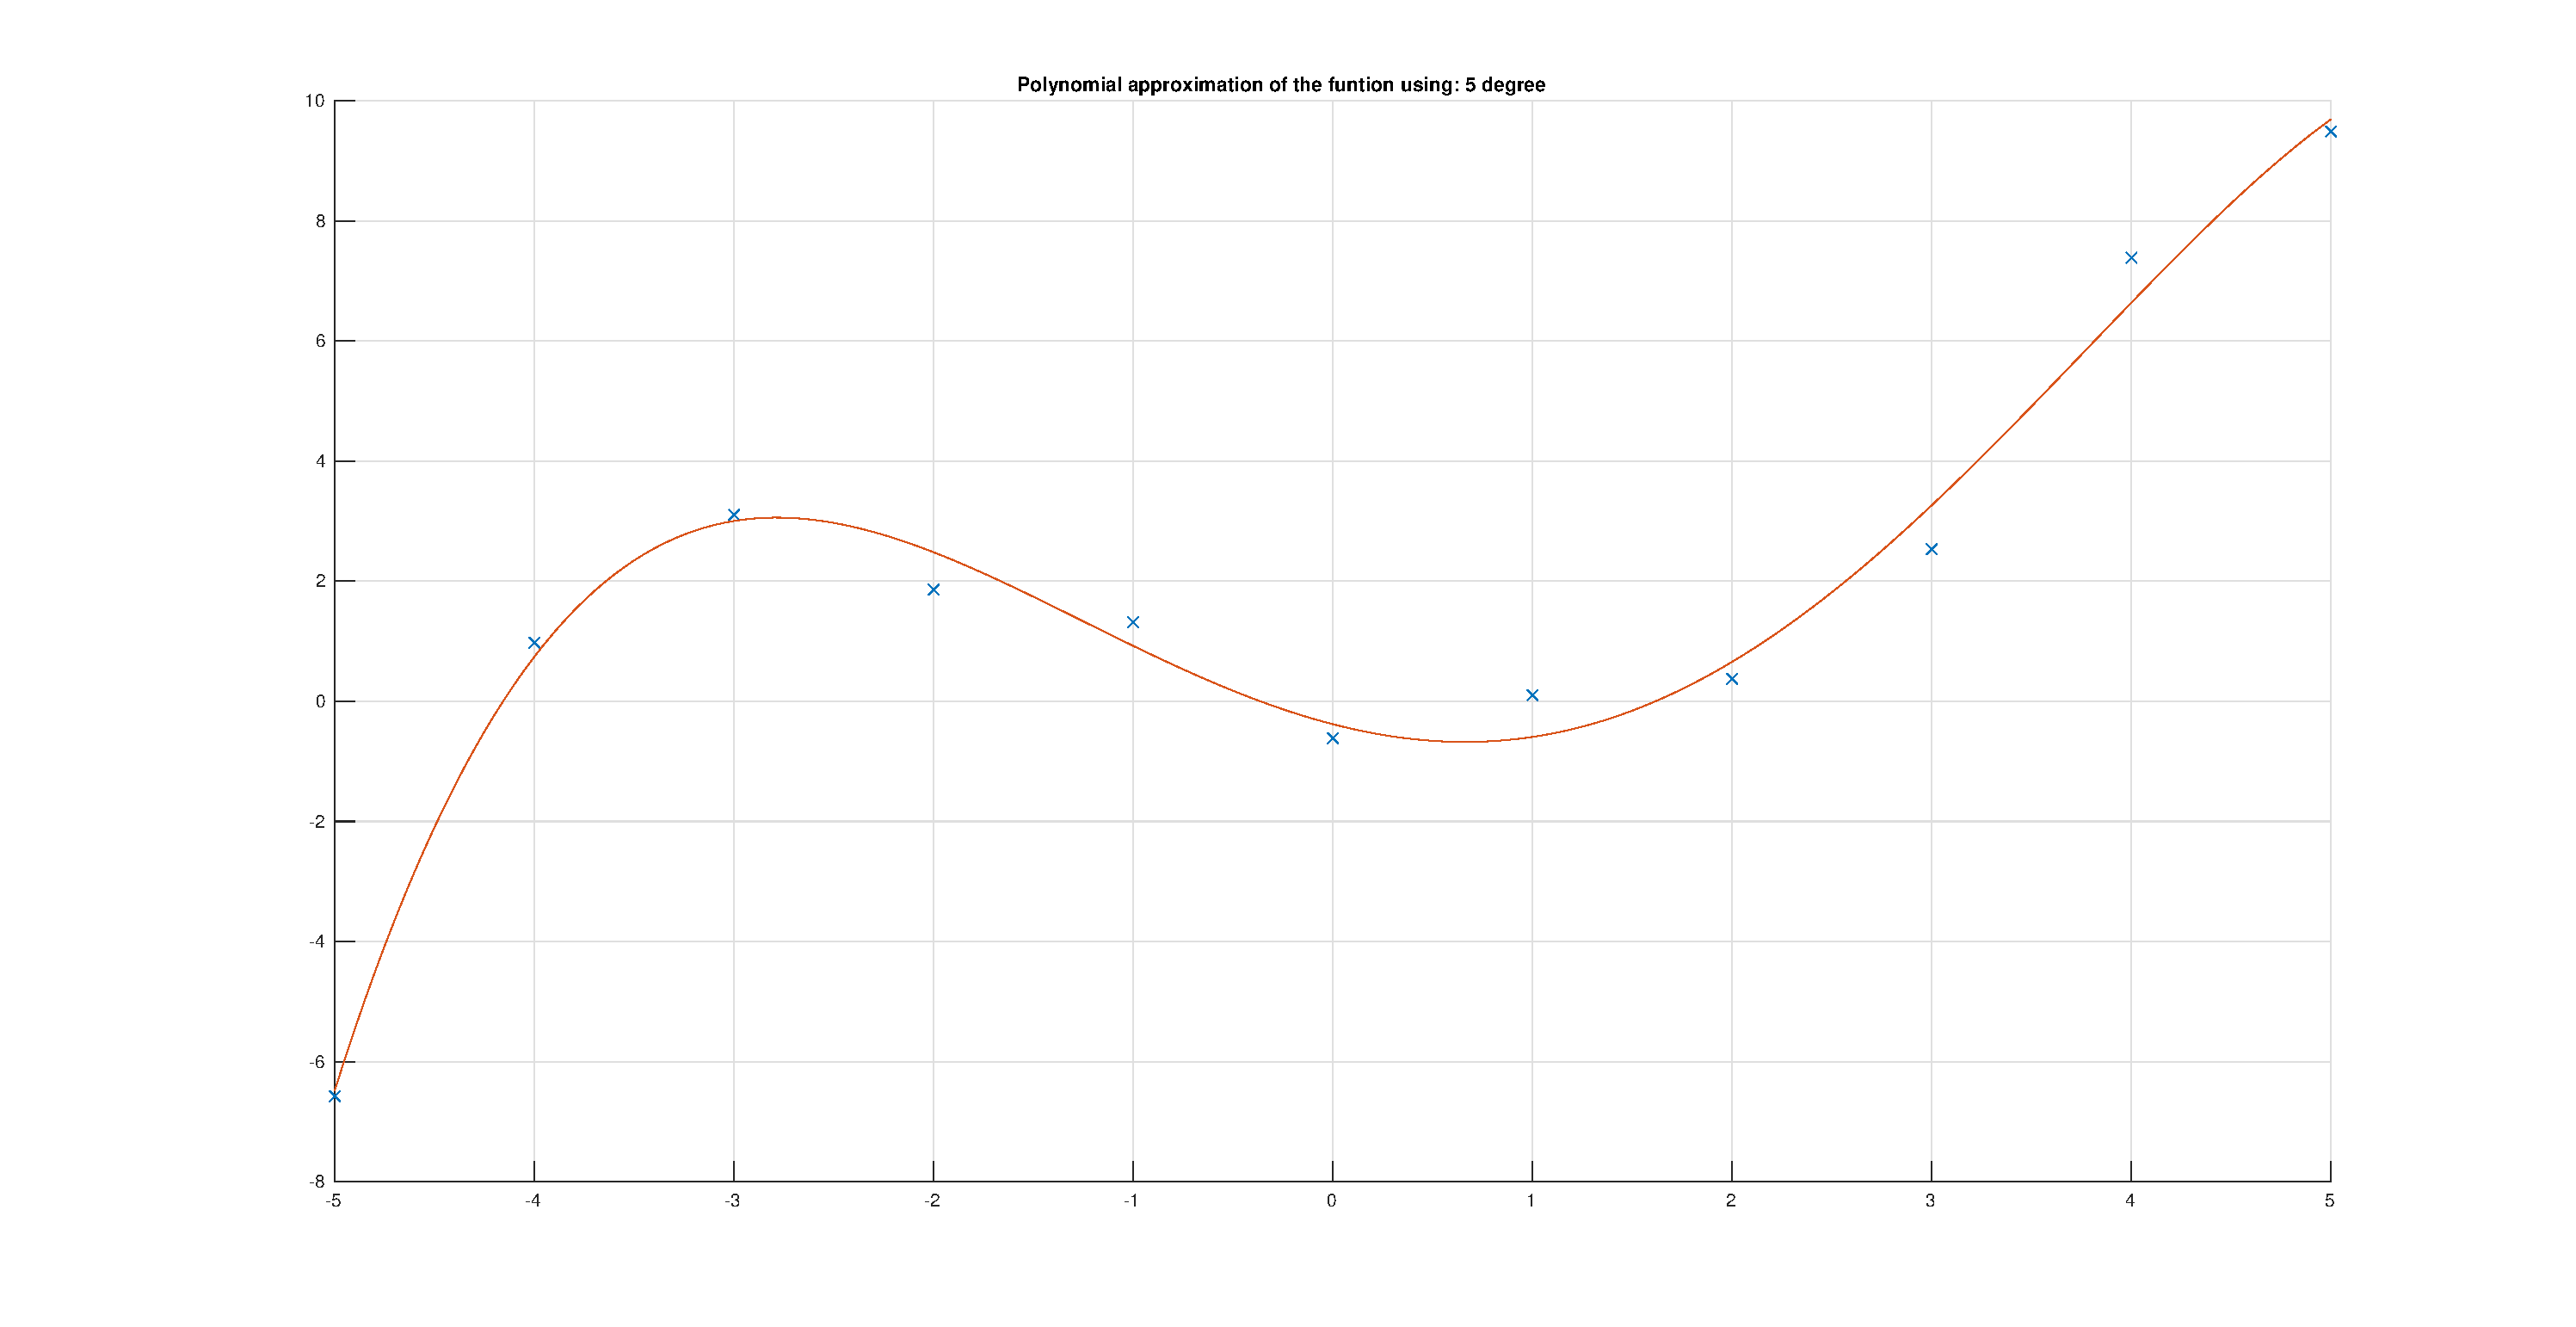
\includepdf[pages=-]{15-eps-converted-to.pdf}
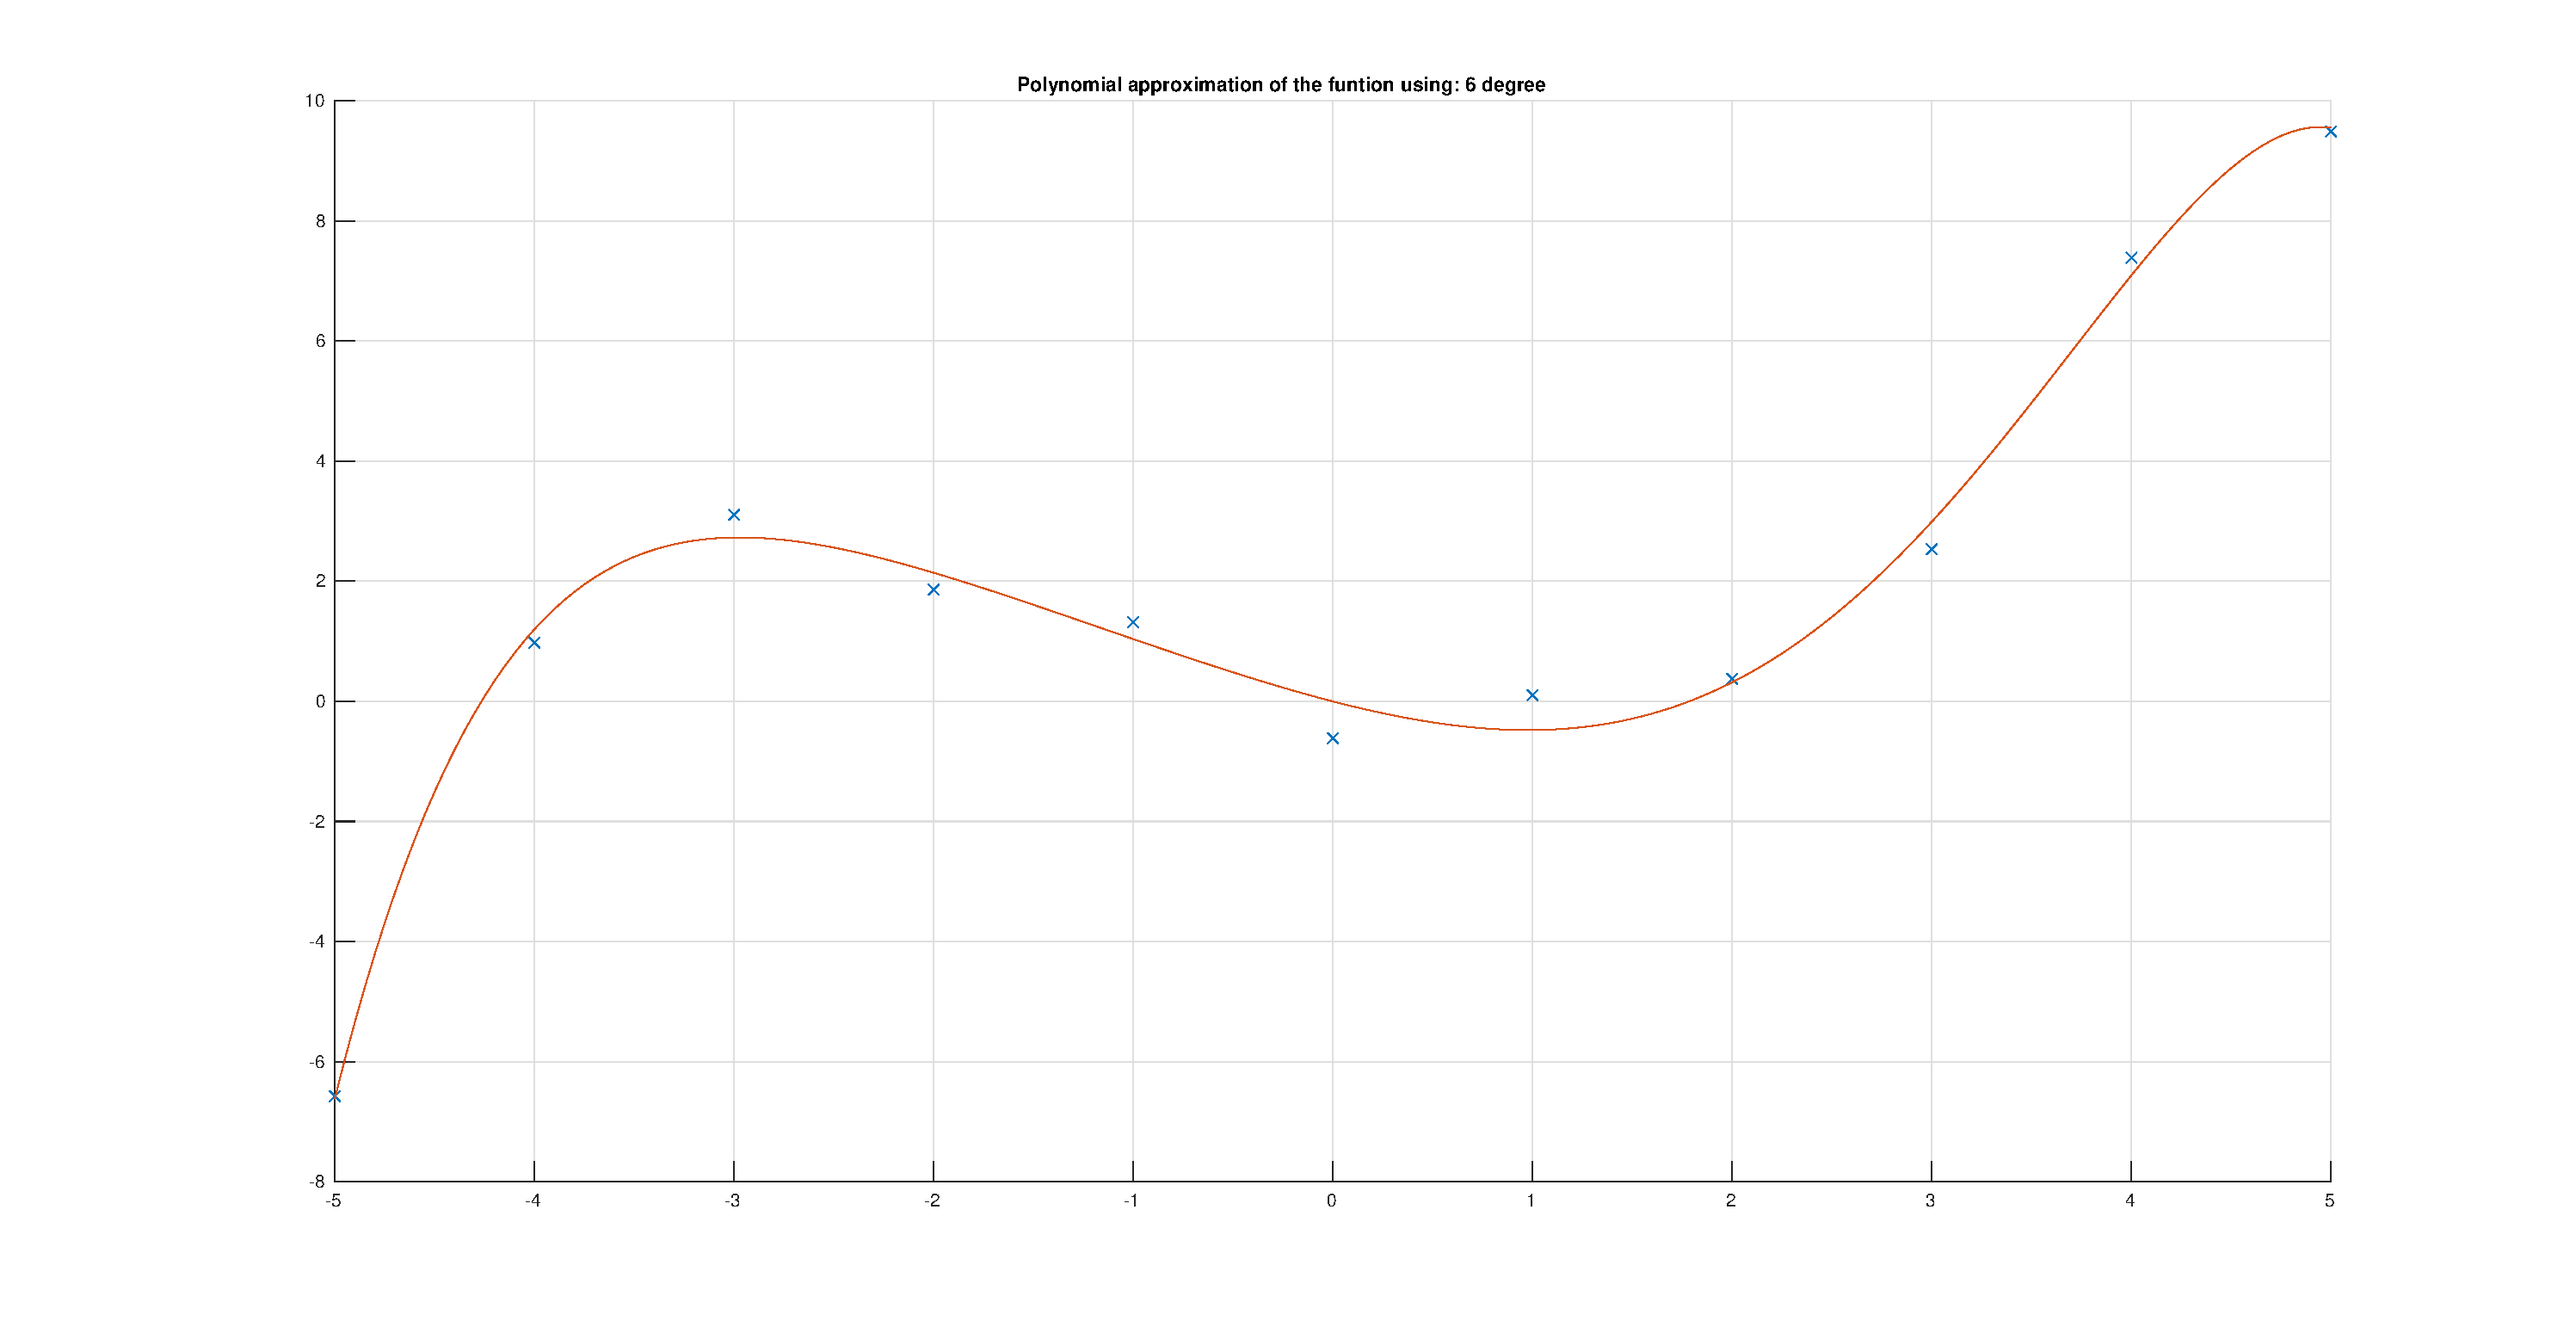
\includepdf[pages=-]{16-eps-converted-to.pdf}
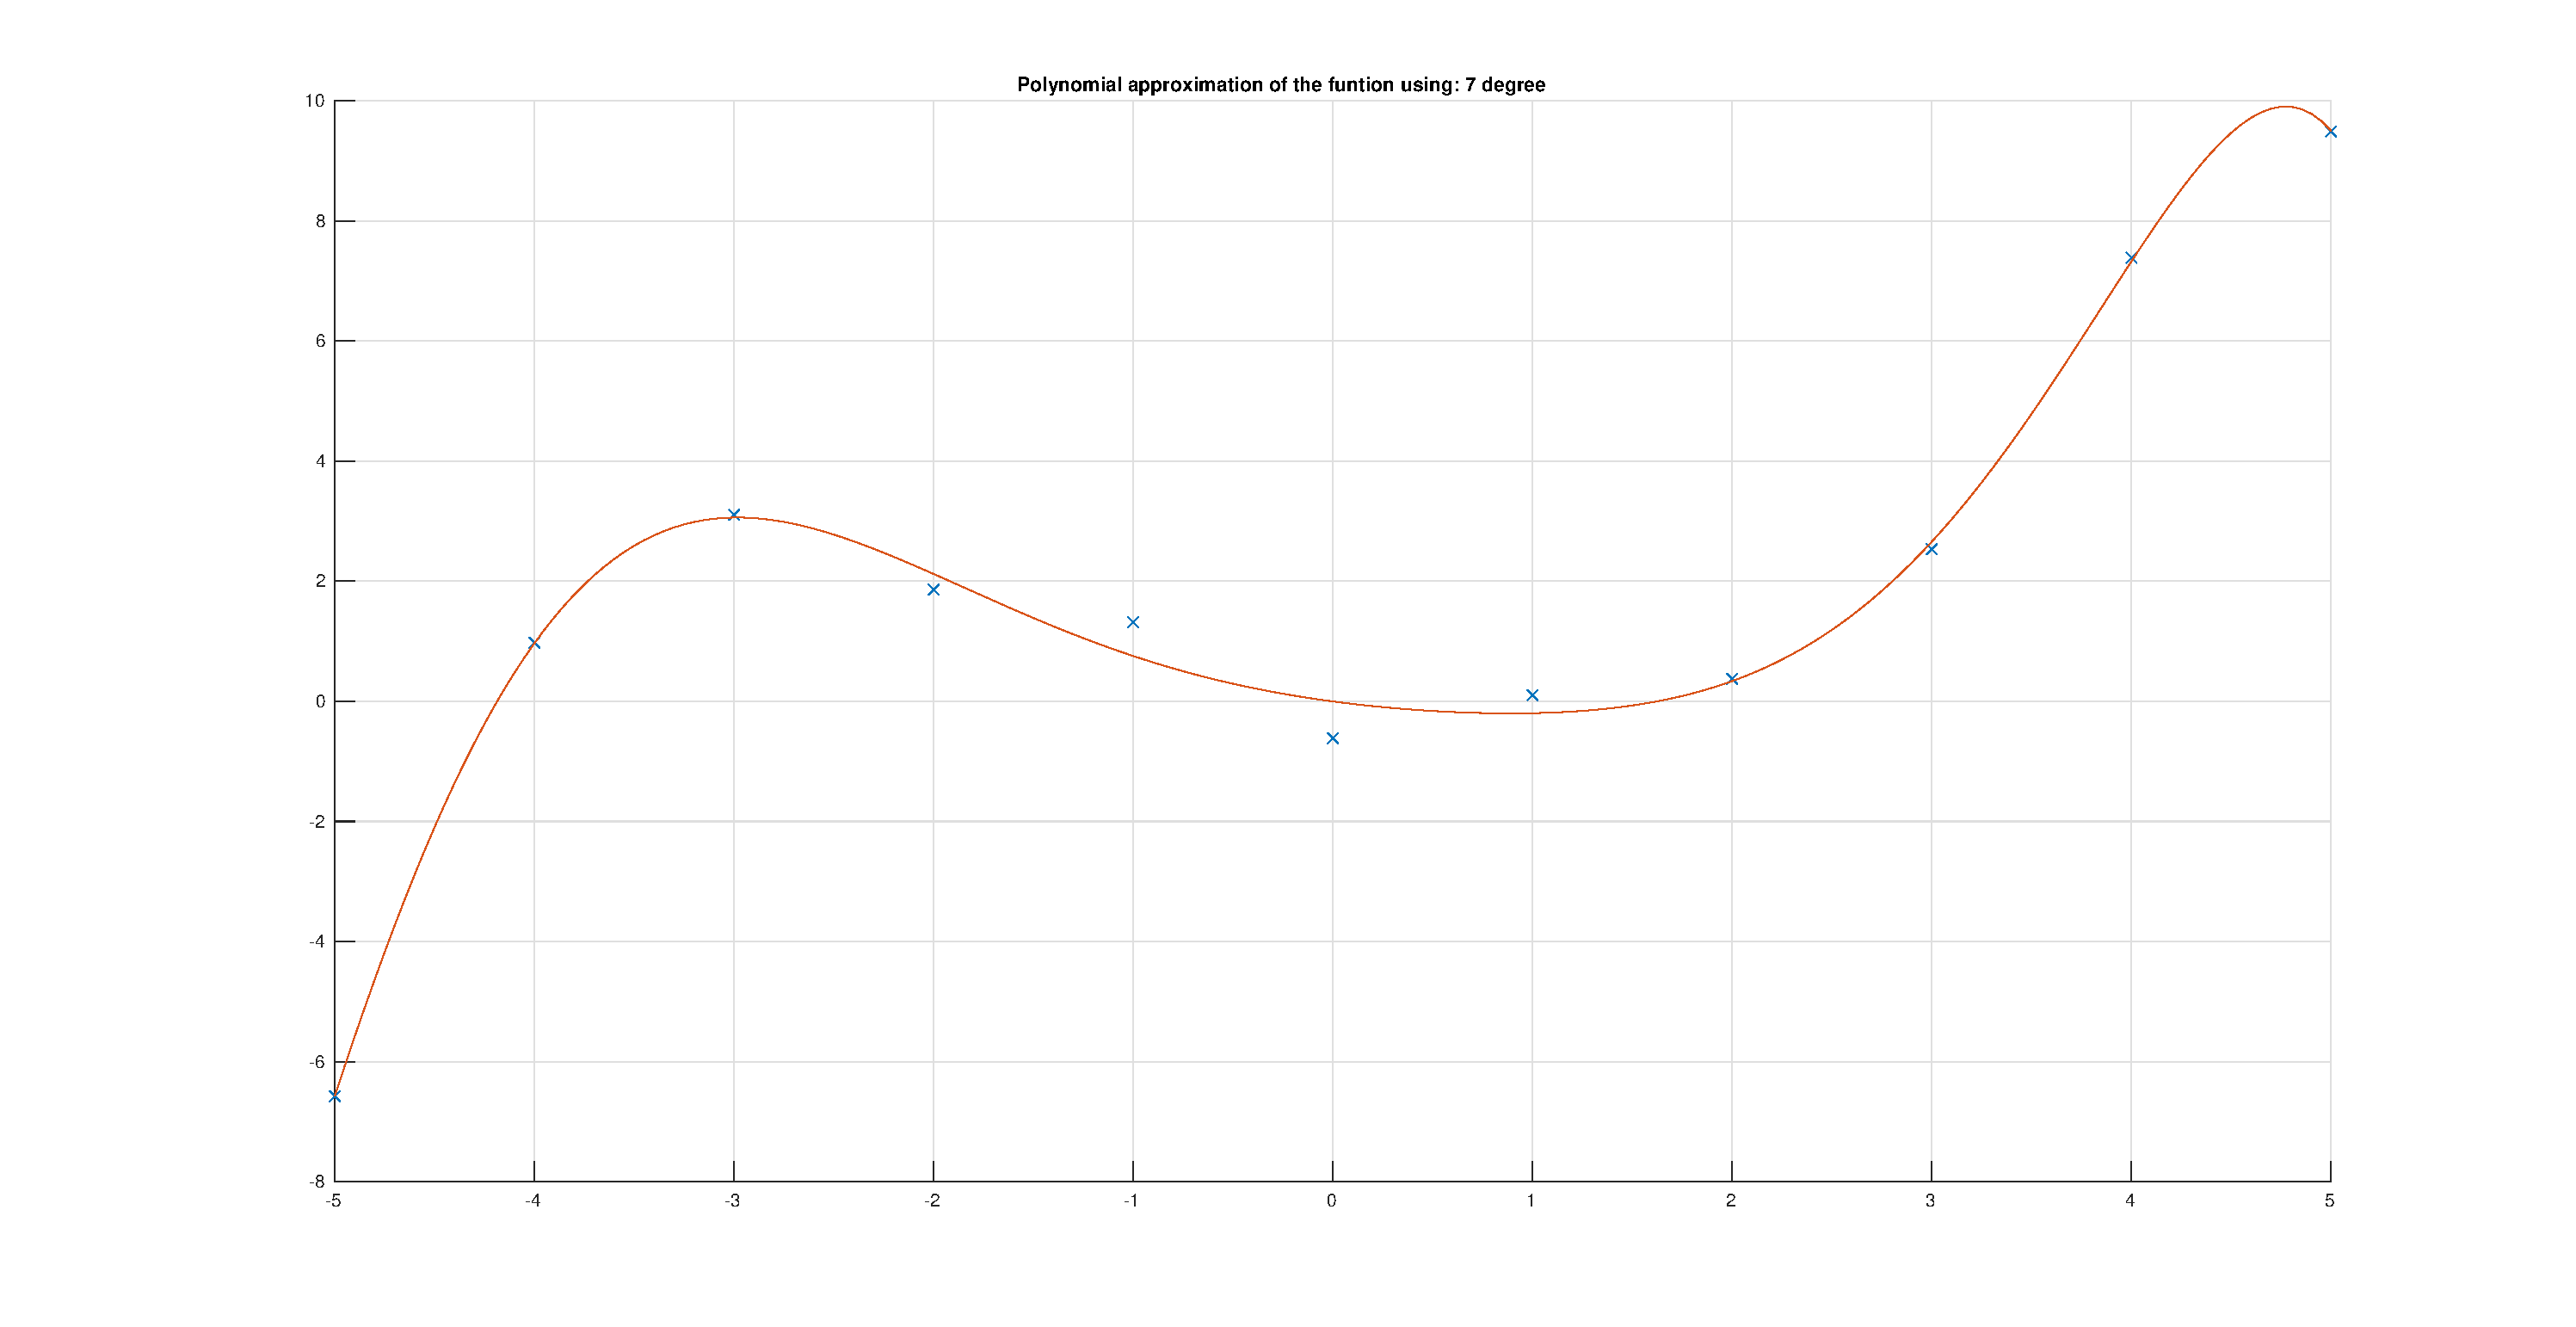
\includepdf[pages=-]{17-eps-converted-to.pdf}
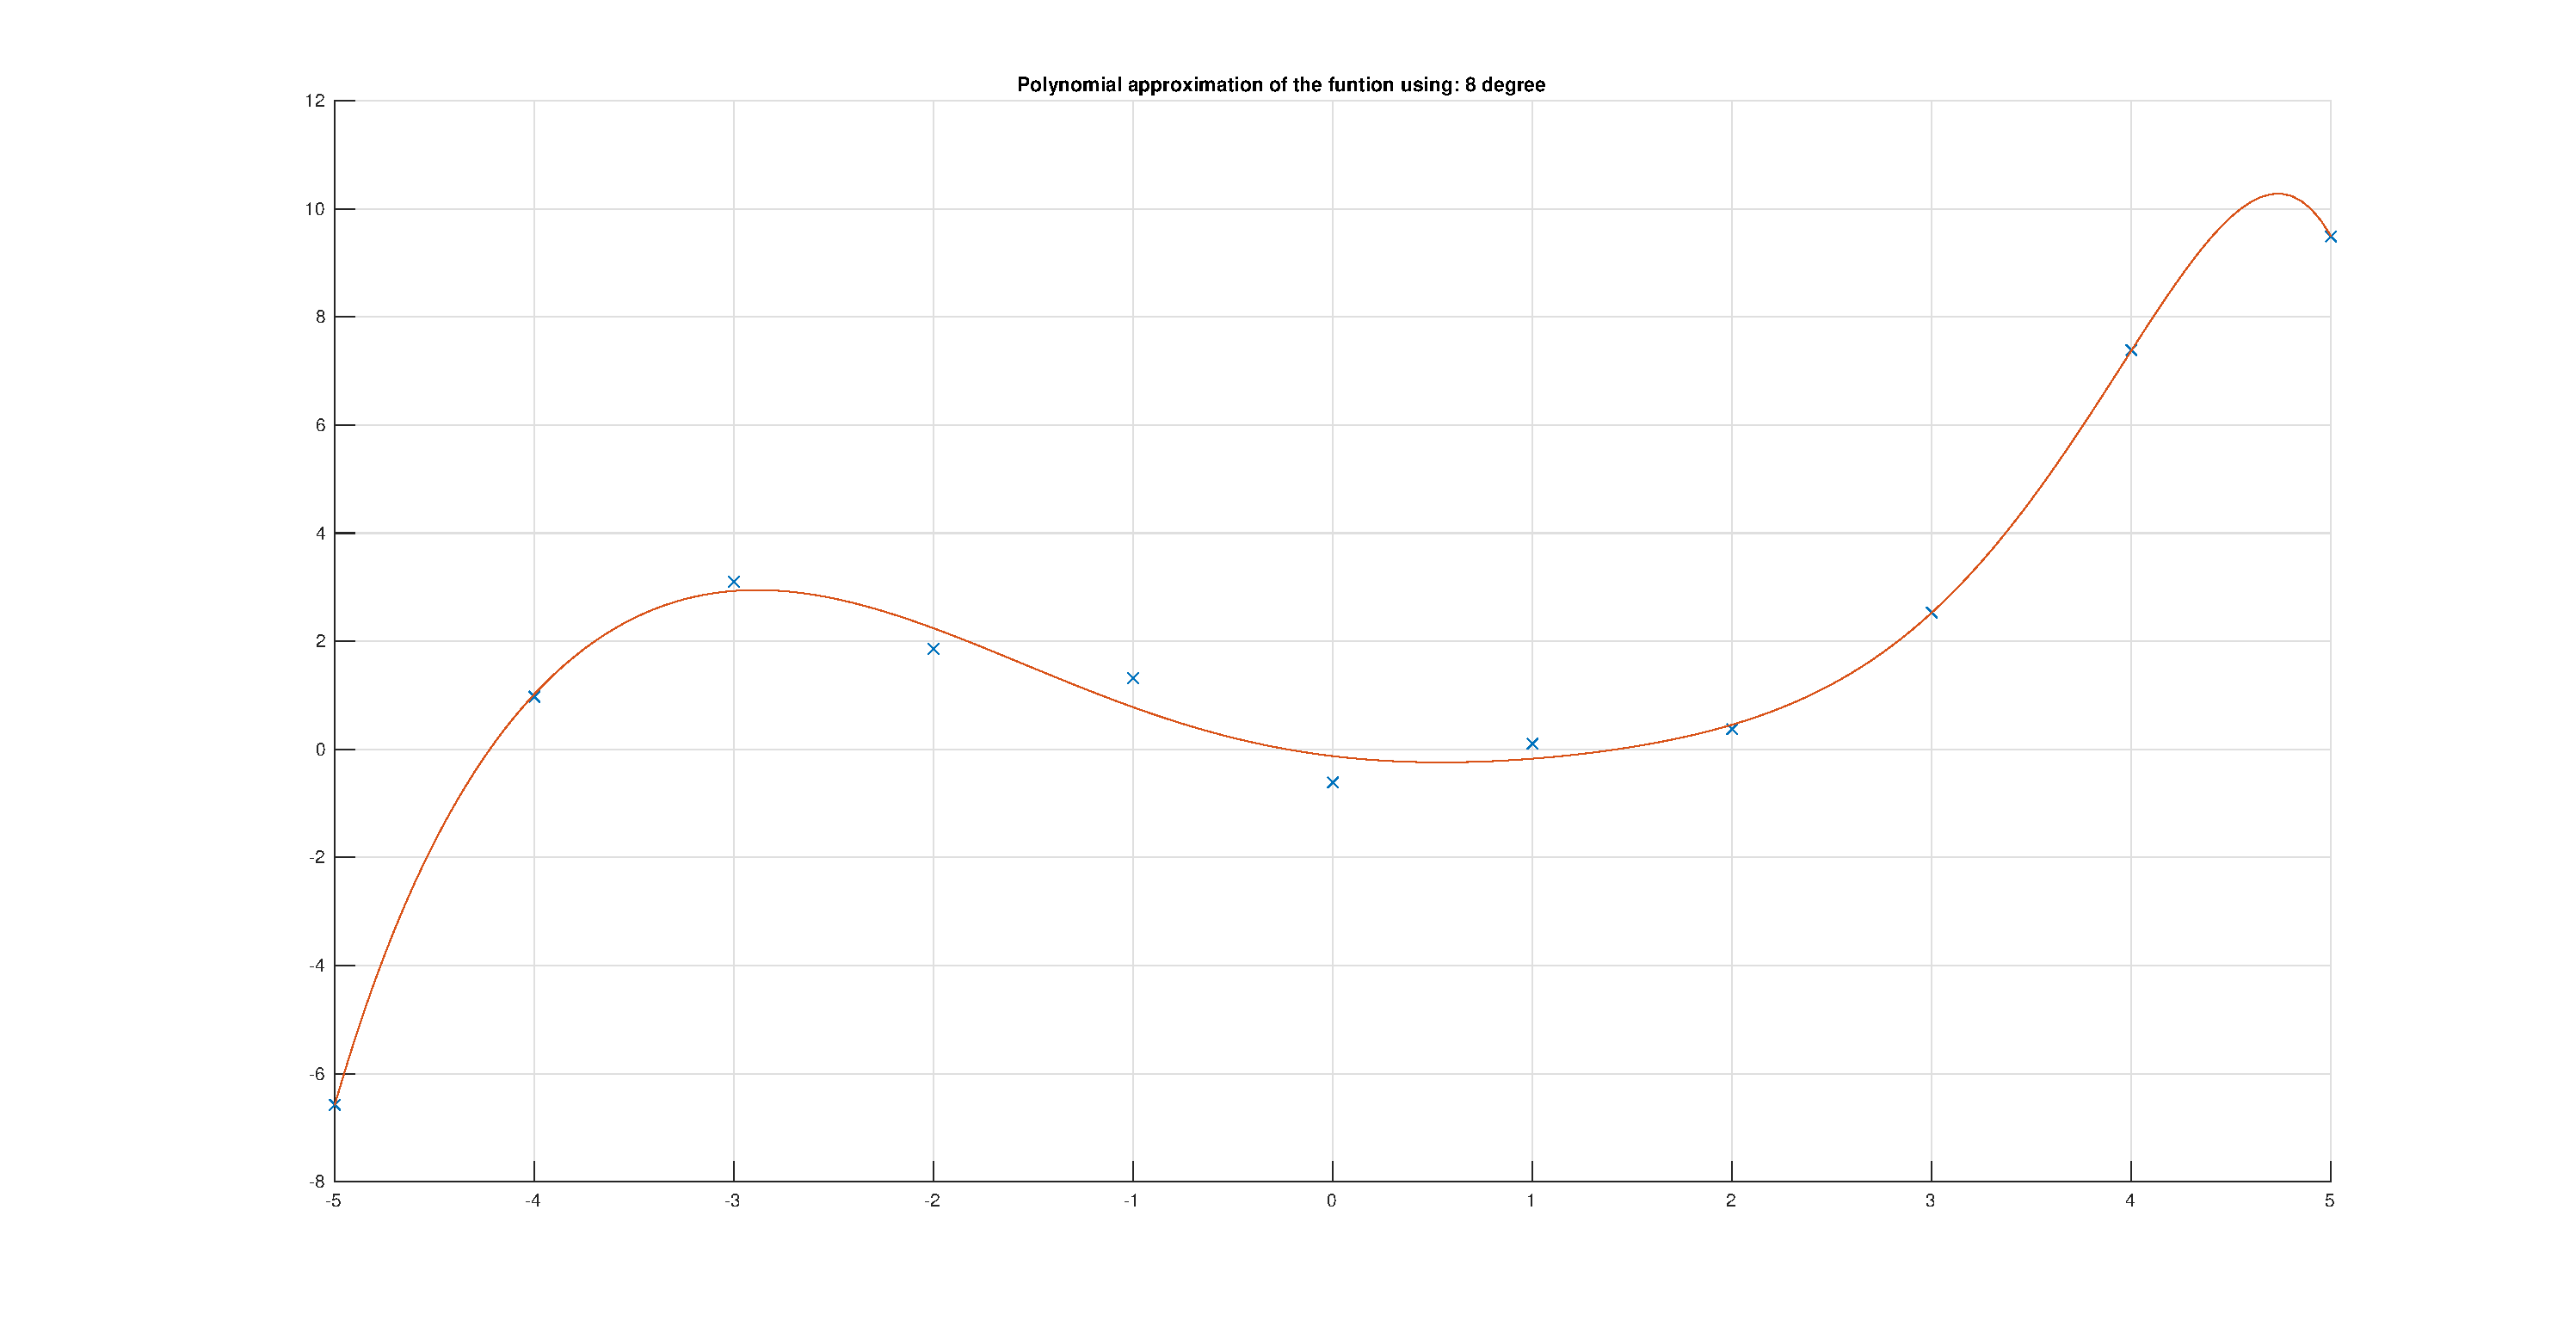
\includepdf[pages=-]{18-eps-converted-to.pdf}
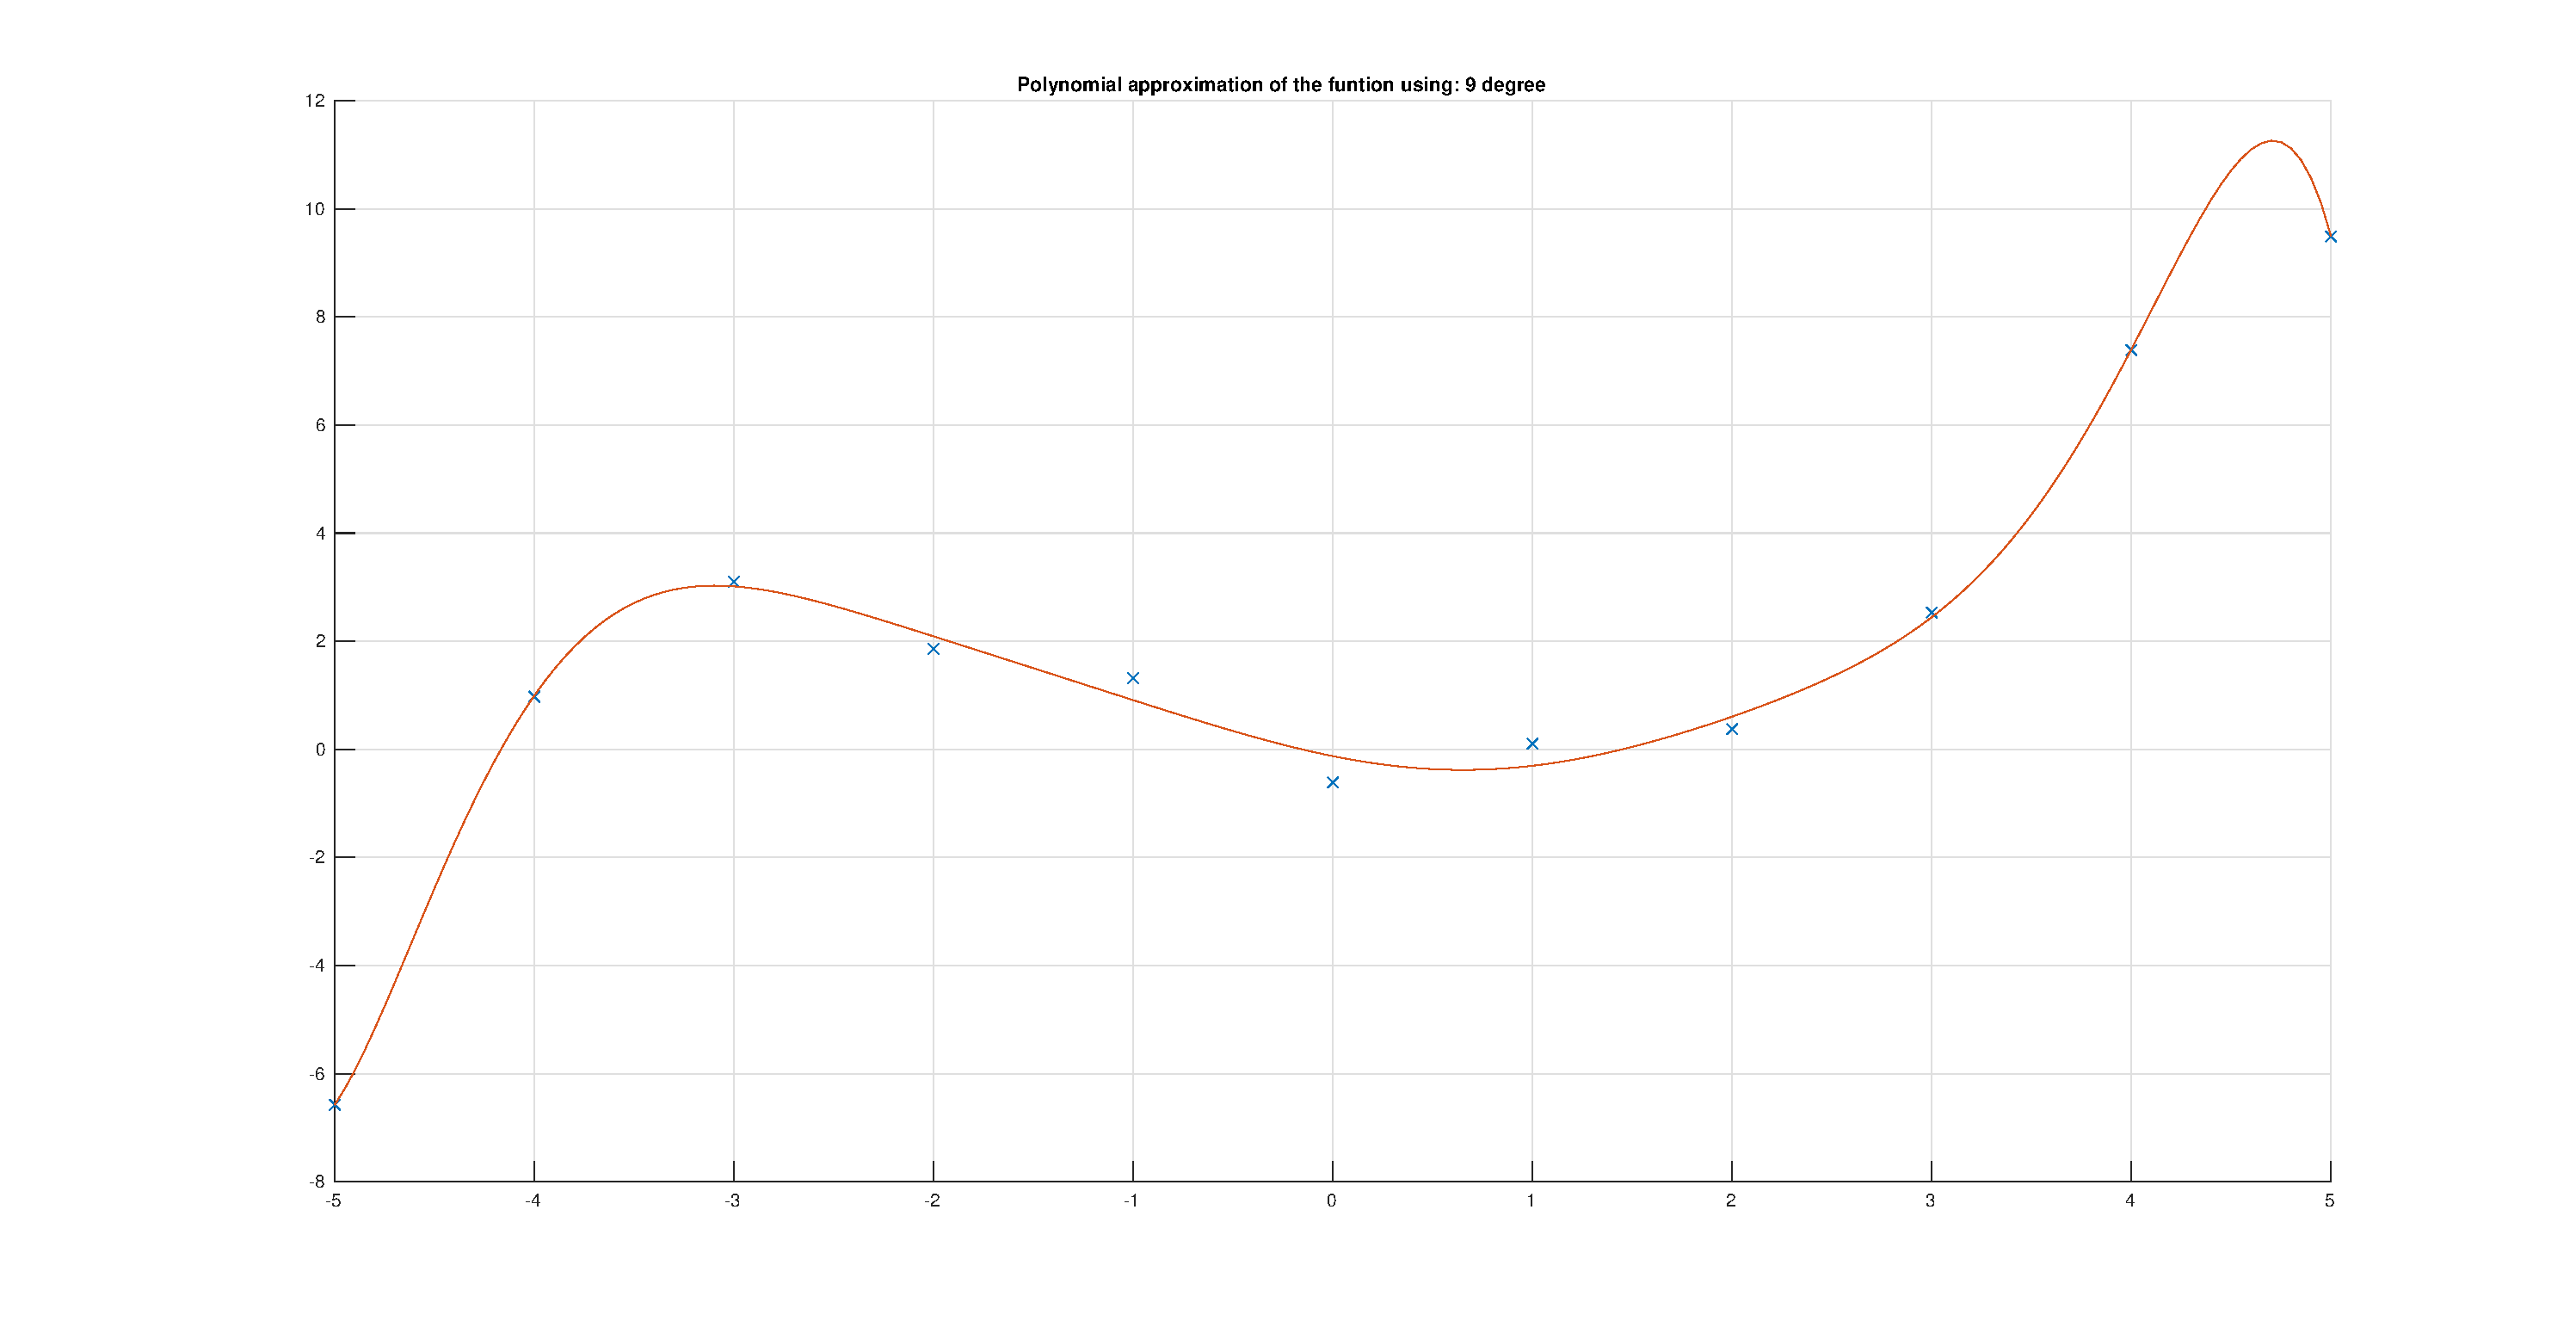
\includepdf[pages=-]{19-eps-converted-to.pdf}
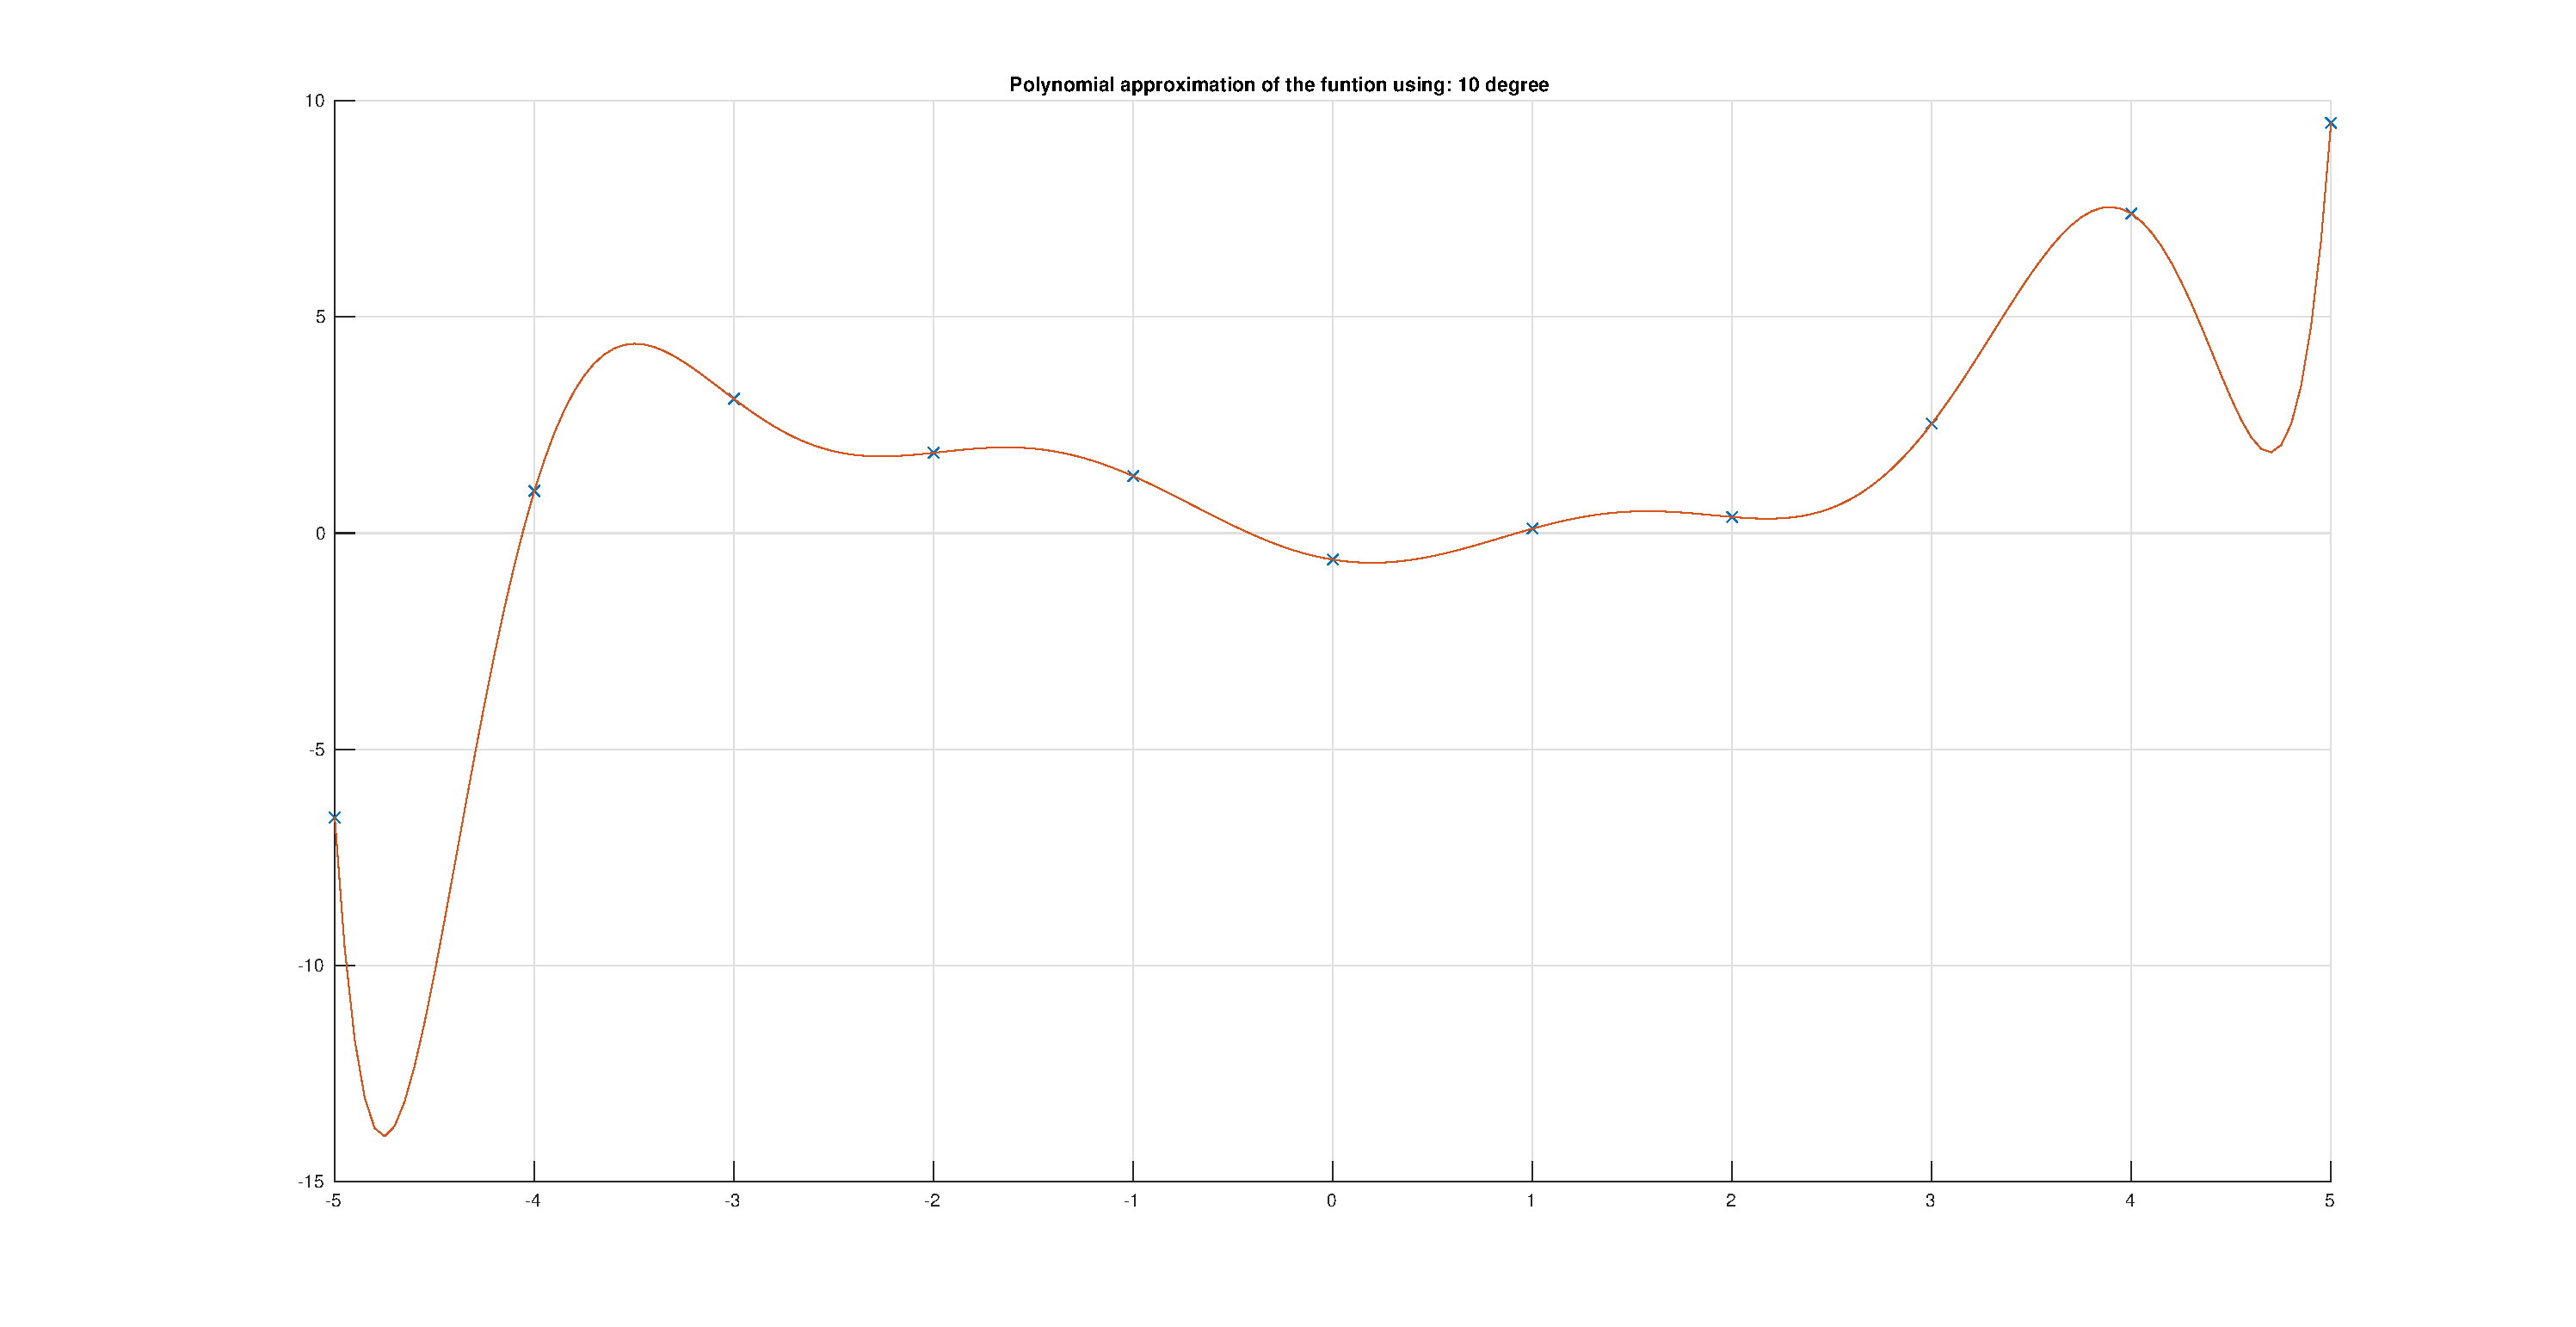
\includepdf[pages=-]{110-eps-converted-to.pdf}
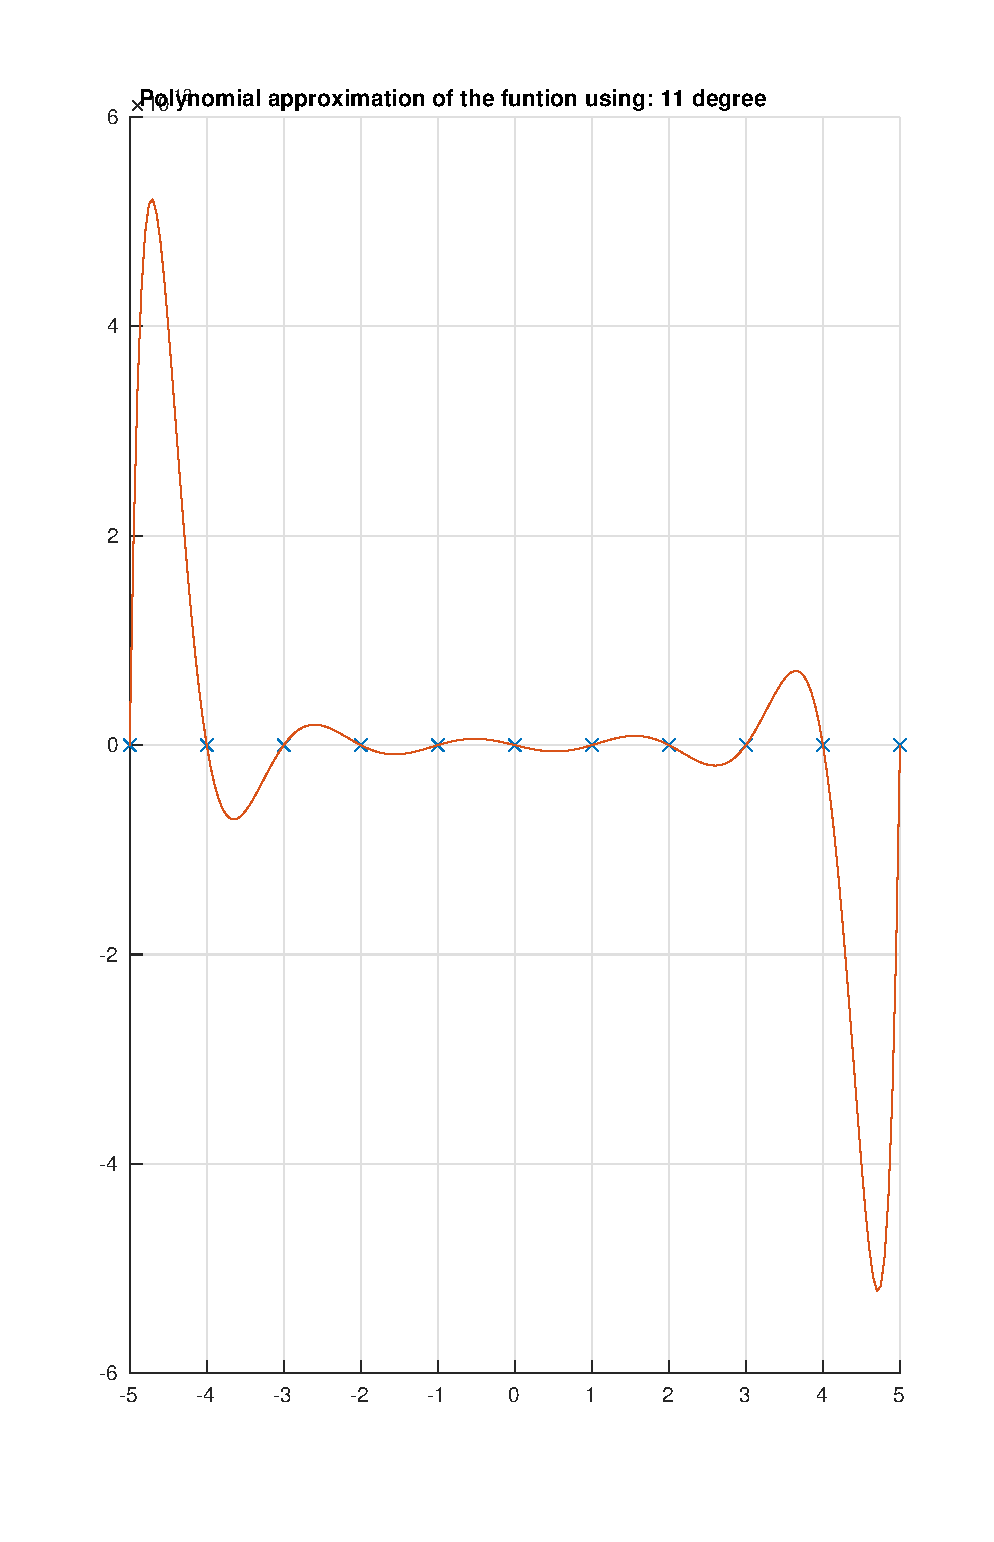
\includepdf[pages=-]{111-eps-converted-to.pdf}

\begin{center}
  \begin{tabular}{| c | c | c |}
\hline

Degree & Error & Condition number of Gram's Matrix \\
\hline
0& 13.2040& 1\\
\hline
1& 9.1281& 10\\
\hline
2& 8.8257&   408.7796\\
\hline
3& 4.2365& 8.5584e+03\\
\hline
4& 1.5418&  3.1798e+05\\
\hline
5& 1.5413& 7.4675e+06\\
\hline
6& 1.1689& 2.8316e+08\\
\hline
7& 0.9345& 7.6462e+09\\
\hline
8& 0.8883& 3.3055e+11\\
\hline
9& 0.8334& 1.5167e+13\\
\hline
10& 6.3645e-13& 9.2930e+14\\
\hline
11 & 2.2390 & 8.7763e+17 \\
\hline
  \end{tabular}
\end{center}

\section{Discussion of results}
As expected, with the increase in polynomial degree error of the solution decreased and condion number of Gram's matrix increased. The most interesting part is how for polynomial of degree \textbf{10} the error got significantly lower, $10^{-12}$ times lower than for polynomial of lower degree, with only around 100 times bigger Gram's matrix condition number, and then for polynomial of degree 11, the error become much much higher and so did Gram's matrix. I suppose that since we get 11 data points, approaching number of data points with the degree of the polynomial lowers the erorr until we have the same polynomial degree as data points at which point the error increases again.






\chapter{Determine trajectory of the motion}


\section{a) Runge-Kutta method of $4^{th}$ order and Adams PC}
\subsection{Problem}
We are given following equations:
\[ \frac{dx_1}{dt} = x_2 + x_1(0.5 - x_1^2 - x_2^2) \]
\[ \frac{dx_2}{dt} = -x_1 + x_2(0.5 - x_1^2 - x_2^2) \]

And we have to determine the trajectory of the motion on interval $[0, 15]$ with following initial conditions:
$ x_1(0) = 8; x_2(0) = 9 $
In this section we will use Runge-Kutta method of $4^{th}$ order and Adams PC with different step-sizes until we find an optimal constant step size - when the decrease of the step size does not influence the solution significantly.

\subsection{Theoretical Introdution}
Determining the trajectory of the motion in this example can be mathematically described as solving a system of first order ordinary differential equations with given initical conditions. That is why we use Runge-Kutta method of order 4 which deals with exactly this kind of problem.
\subsubsection{Runge-Kutta method of order 4}
Any single step method are defined by the following formula, where h is a fixed step-size:
\[ y_{n+1} = y_n + \Phi_f(x_n, y_n, h) \]
where:
\[ x_n = x_0 + nh \]
\[ y(x_0) = y_0 = y_a \]
where $y_a$ is given.
Runge-Kutta method of order 4 - RK4 method looks like this:
\[ y_{n+1} = y_n + \frac{1}{6}(k_1 + 2k_2+2k_3+k_4) \]
\[ k_1 = f(x_n, y_n) \]
\[ k_3 = f(x_n + \frac{1}{2}h, y_n + \frac{1}{2}hk_1) \]
\[ k_2 = f(x_n + \frac{1}{2}h, y_n + \frac{1}{2}hk_2) \]
\[ k_4 = f(x_n + h, y_n + hk_3) \]


\subsection{Adams PC method}
Adams method with $P_kEC_kE$ algorithm has the following form: \\
P: \[  y_n^{[0]} = y_{n-1} + h\sum_{j=1}^k \beta_jf_{n-j} \]
E: \[  f_n^{[0]} = f(x_n, y_n^{[0]}) \]
C: \[  y_n = y_{n-1} + h \sum_{j=1}^k \beta_j^* f_{n-j} + h \beta_0^* f_n^{[0]}\]
E: \[  f_n = f(x_n, y_n) \]

When compared to explicit and implicit adams method PC metho has smaller absolute stability intervals than implicit method, while having significant advantage in calculations cost.



\section{b) Runge-Kutta method of $4^{th}$ order with variable step size automatically adjusted}
\subsection{Problem}
We are given following equations:
\[ \frac{dx_1}{dt} = x_2 + x_1(0.5 - x_1^2 - x_2^2) \]
\[ \frac{dx_2}{dt} = -x_1 + x_2(0.5 - x_1^2 - x_2^2) \]
And we have to determine the trajectory of the motion on interval $[0, 15]$ with following initial conditions:
$ x_1(0) = 8; x_2(0) = 9 $
In this section we will use Runge-Kutta method of $4^{th}$ order with step size automatically adjusted by the algorithm, with error estimation made according to the step-doubling rule.
\subsection{Theoretical Introdution}
Since Runge-Kutta method was explained in previous task I will focus on step-doubling rule.
Everytime we increase step size we receive less accurate results at the benefit of less calculations cost, this means that we need to have reasonable approach to setting step size to maximise accuracy and minimize calculations cost. We will use step-doubling rule in this example.

\subsubsection{Error estimation using step doubling-approach}
For every step of size $h$ we perform two additional steps of size $\frac{h}{2}$. We denote: \\
$y_n^{1}$ as a new point obtained using the original step-size $h$ \\
$y_n^{2}$ as a new point obtained using steps of the size $\frac{h}{2}$ \\
$r^{(1)}$ - approximation error affter the single step $h$ \\
$r^{(2)}$ - summed approximation errors after the two smaller steps of length $\frac{h}{2}$ each. \\
We have: \\
\newpage
After a single step:
\[ y(x_n + h) = y_n^{(1)} + \frac{r_n^{p+1}(0)}{(p+1)!}h^{p+1} + O(h^{p+2}) \]
After a double step:
\[  y(x_n+h) \simeq y_n^{(2)} + 2\frac{r_n^{p+1}(0)}{(p+1)!}(\frac{h}{2})^{p+1} + O(h^{p+2}) \]

We evaluate unknown coefficient from the first equation $ \frac{r_n^{p+1}(0)}{(p+1)!} $ and insert it into second one:
\[ y(x_n+h) = y_n^{(2)} + \frac{h^{p+1}}{2^p}\frac{(x_n+h) - y_n^{(1)}}{h^{p+1} + O(h^{p+2})} \]
We continue further and receive:
\[ y(x_n + h)(1-\frac{1}{2^p}) = y_n^{(2)}(1-\frac{1}{2^p}) + \frac{y_n^{2}}{2^p} - \frac{y_n^{(1)}}{2^p} + O(h^{p+2}) \]
We multiply by $\frac{2^p}{2^p - 1}$ and get:
\begin{equation}
y(x_n+h) = y_n^{(2)} + \frac{ y_n^{(2)} - y_n^{(1)} }{ 2^p - 1 } + O(h^{p+2})
\end{equation}
We also obtain for first equation in a similar way:
 \[ y(x_n+h) = y_n^{(1)} + 2^p\frac{y_n^{(2)} - y_n^{(1)}}{2^p - 1} + O(h^{p+2}) \]
Assuming we take the main part of the error we get error estimate:
\[ \delta_n(h) = \frac{2^p}{2^p-1}(y_n^{(2)} - y_n^{(1)}) \]
But from the equation (2.1) we can treat expression:
\[ \delta_n(2 \times \frac{h}{2}) = \frac{ y_n^{(2)} - y_n^{(1)}}{2^p - 1} \]
as en estimate of the error of two consecutive steps of size $\frac{h}{2}$
\subsubsection{Actual correction of the step size}
In general formula for main part of the approximation error where:
\\ $h$ - length of a step
\[ \gamma = \frac{r_n^{(p+1)}(0)}{(p+1)!} \]
Looks like this:
\[ \delta_n(h) = \gamma h^{p+1} \]
If we change step-size to $\alpha h$ then we get:
\[ \delta_n(\alpha h) = \gamma (\alpha h)^{p+1} \]
Then:
\[ \delta_n(\alpha h) = \alpha^{p+1} \delta_n (h) \]
We assume tolerance $\epsilon$:
\[ |\delta_n(\alpha h)| = \epsilon \]
We get:
\[ \alpha^{p+1}|\delta_n(h)| = \epsilon \]
Coefficient $\alpha$ for the step-size correction can be evaluated in such a way:
\[ \alpha = (\frac{\epsilon}{|\delta_n (h)|})^{\frac{1}{p+1}} \]

This method is also correct for RK4 method when $\delta_n(h) = \delta_n(2 \times \frac{h}{2}) $
We should also take into considertaion lack of accuracy we do so by using safety factor $s$:
\[ h_{n+1} = s \alpha h_n \]
where $ s < 1 $
For RK4 we use $ s \approx 0.9 $ \\
We define accuracy parameters in such a way:
\[ \epsilon = |y_n| \epsilon_r + \epsilon_a \]
where $\epsilon_r$ is relative tolerance and $\epsilon_a$ is absolute tolerance. \\
In case of set of more than on differential equations we must use worst case approach so the equations that need smallest step-size define step-size for all other equations.
\newpage
For RK methods we have following parameters:
\[ \delta_n(h)_i = \frac{(y_i)_n^{(2)} - (y_i)_n^{(1)}}{2^p - 1} \]
\[ \epsilon_i = |(y_i)_n^{(2)}| \epsilon_r + \epsilon_a \]
\[ \alpha = \min_{1 \leq i \leq m} (\frac{\epsilon_i}{|\delta_n(h)_i}|)^{\frac{1}{p+1}} \]

\subsection{Flow diagram}
\begin{tikzpicture}[node distance=5cm]
  \node (start) [startstop, align=center]
  {
        START
  \begin{itemize}

    \item Functions from task
    \item Initial values
    \item Initial step size
    \item Integration interval
    \item Absolute error
    \item Relative error
  \end{itemize}
  };
  \node (solution) [align=center, startstop, below of = start]
  {
  Calculate solution:
  \[ x_{n+1} = x_n + h_n \]
  \[ y_{n+1} = y_n + h \phi_f(x_n; y_n; h) \]
  };
  \node (interval) [align=center, io, below of = solution]
  {
  $x_n$ > integration interval?
  };
  \node (finish) [startstop, align=center, , right=3cm of interval] {Finish};
  \node (error) [startstop, align=center, , below of = interval]
  {
  Estimate error and update step size:
  \[ h_{n+1} = s\alpha h_n \]
  };

\path [-stealth, thick]
    (start) edge   (solution);
\path [-stealth, thick]
  (solution) edge   (interval);
\path [-stealth, thick]
  (interval) edge node[anchor=south] {YES}  (finish);
\path [-stealth, thick]
  (interval) edge node[anchor=east] {NO}   (error);
\path [-stealth, thick]
  (error) edge [bend left = 90]   (solution);

\end{tikzpicture}

\section{Results}

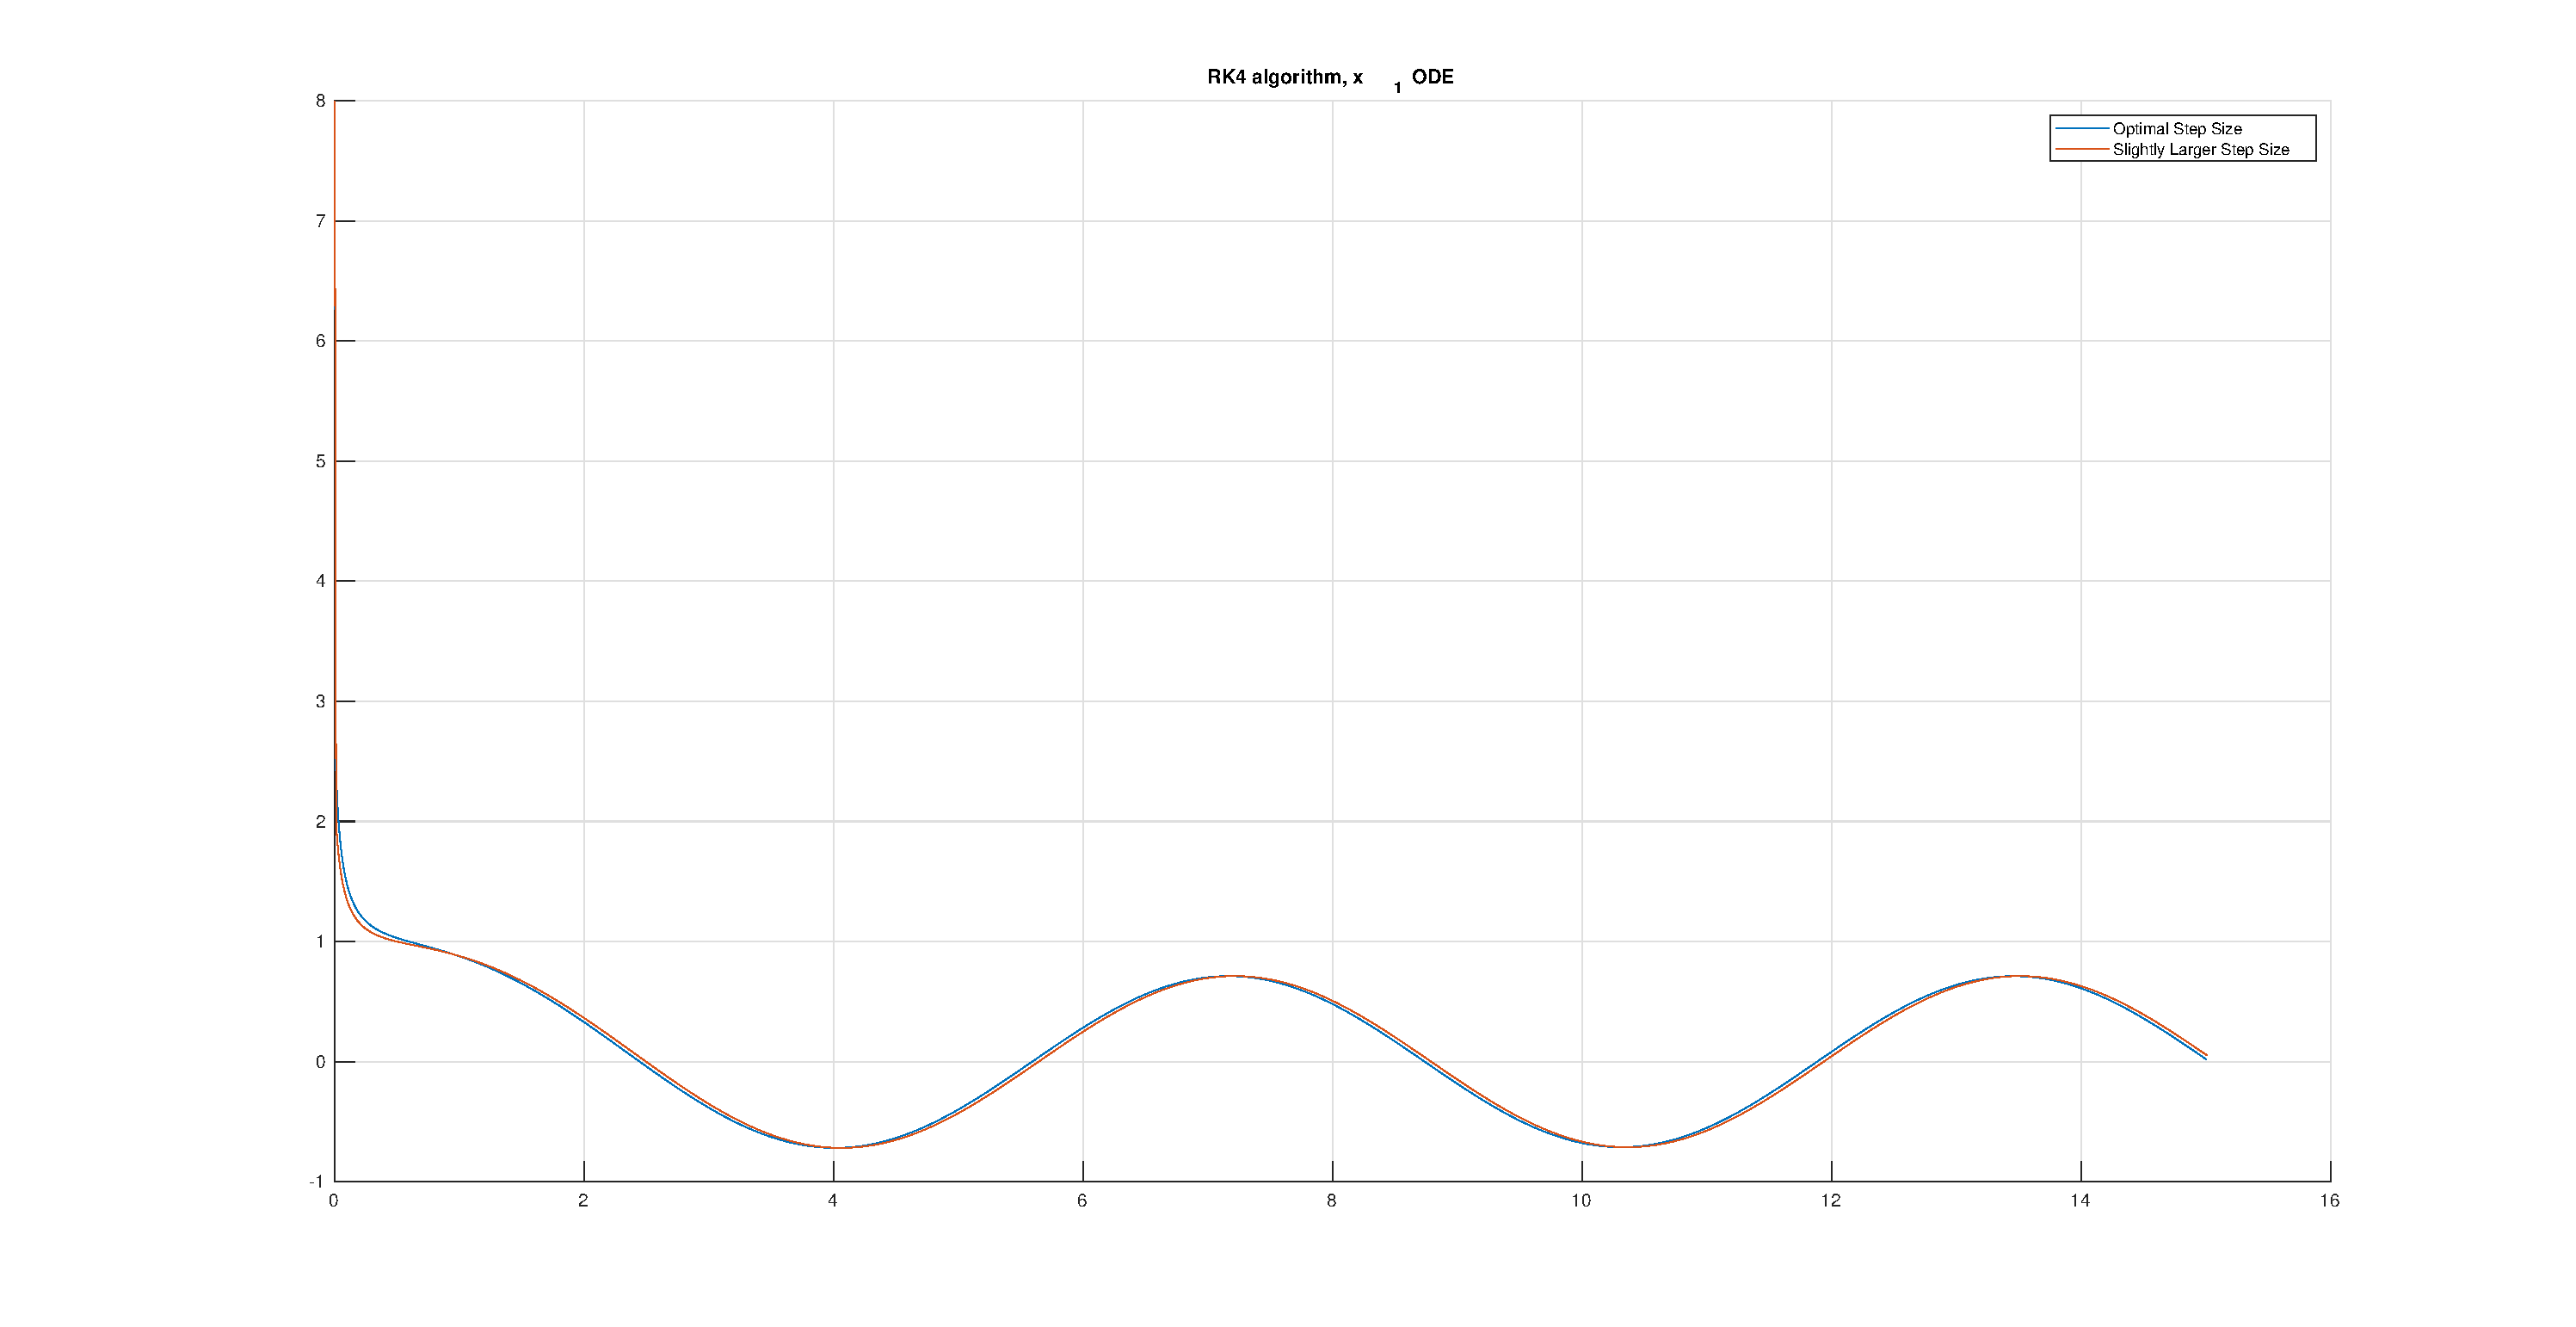
\includepdf[pages=-]{20-eps-converted-to.pdf}
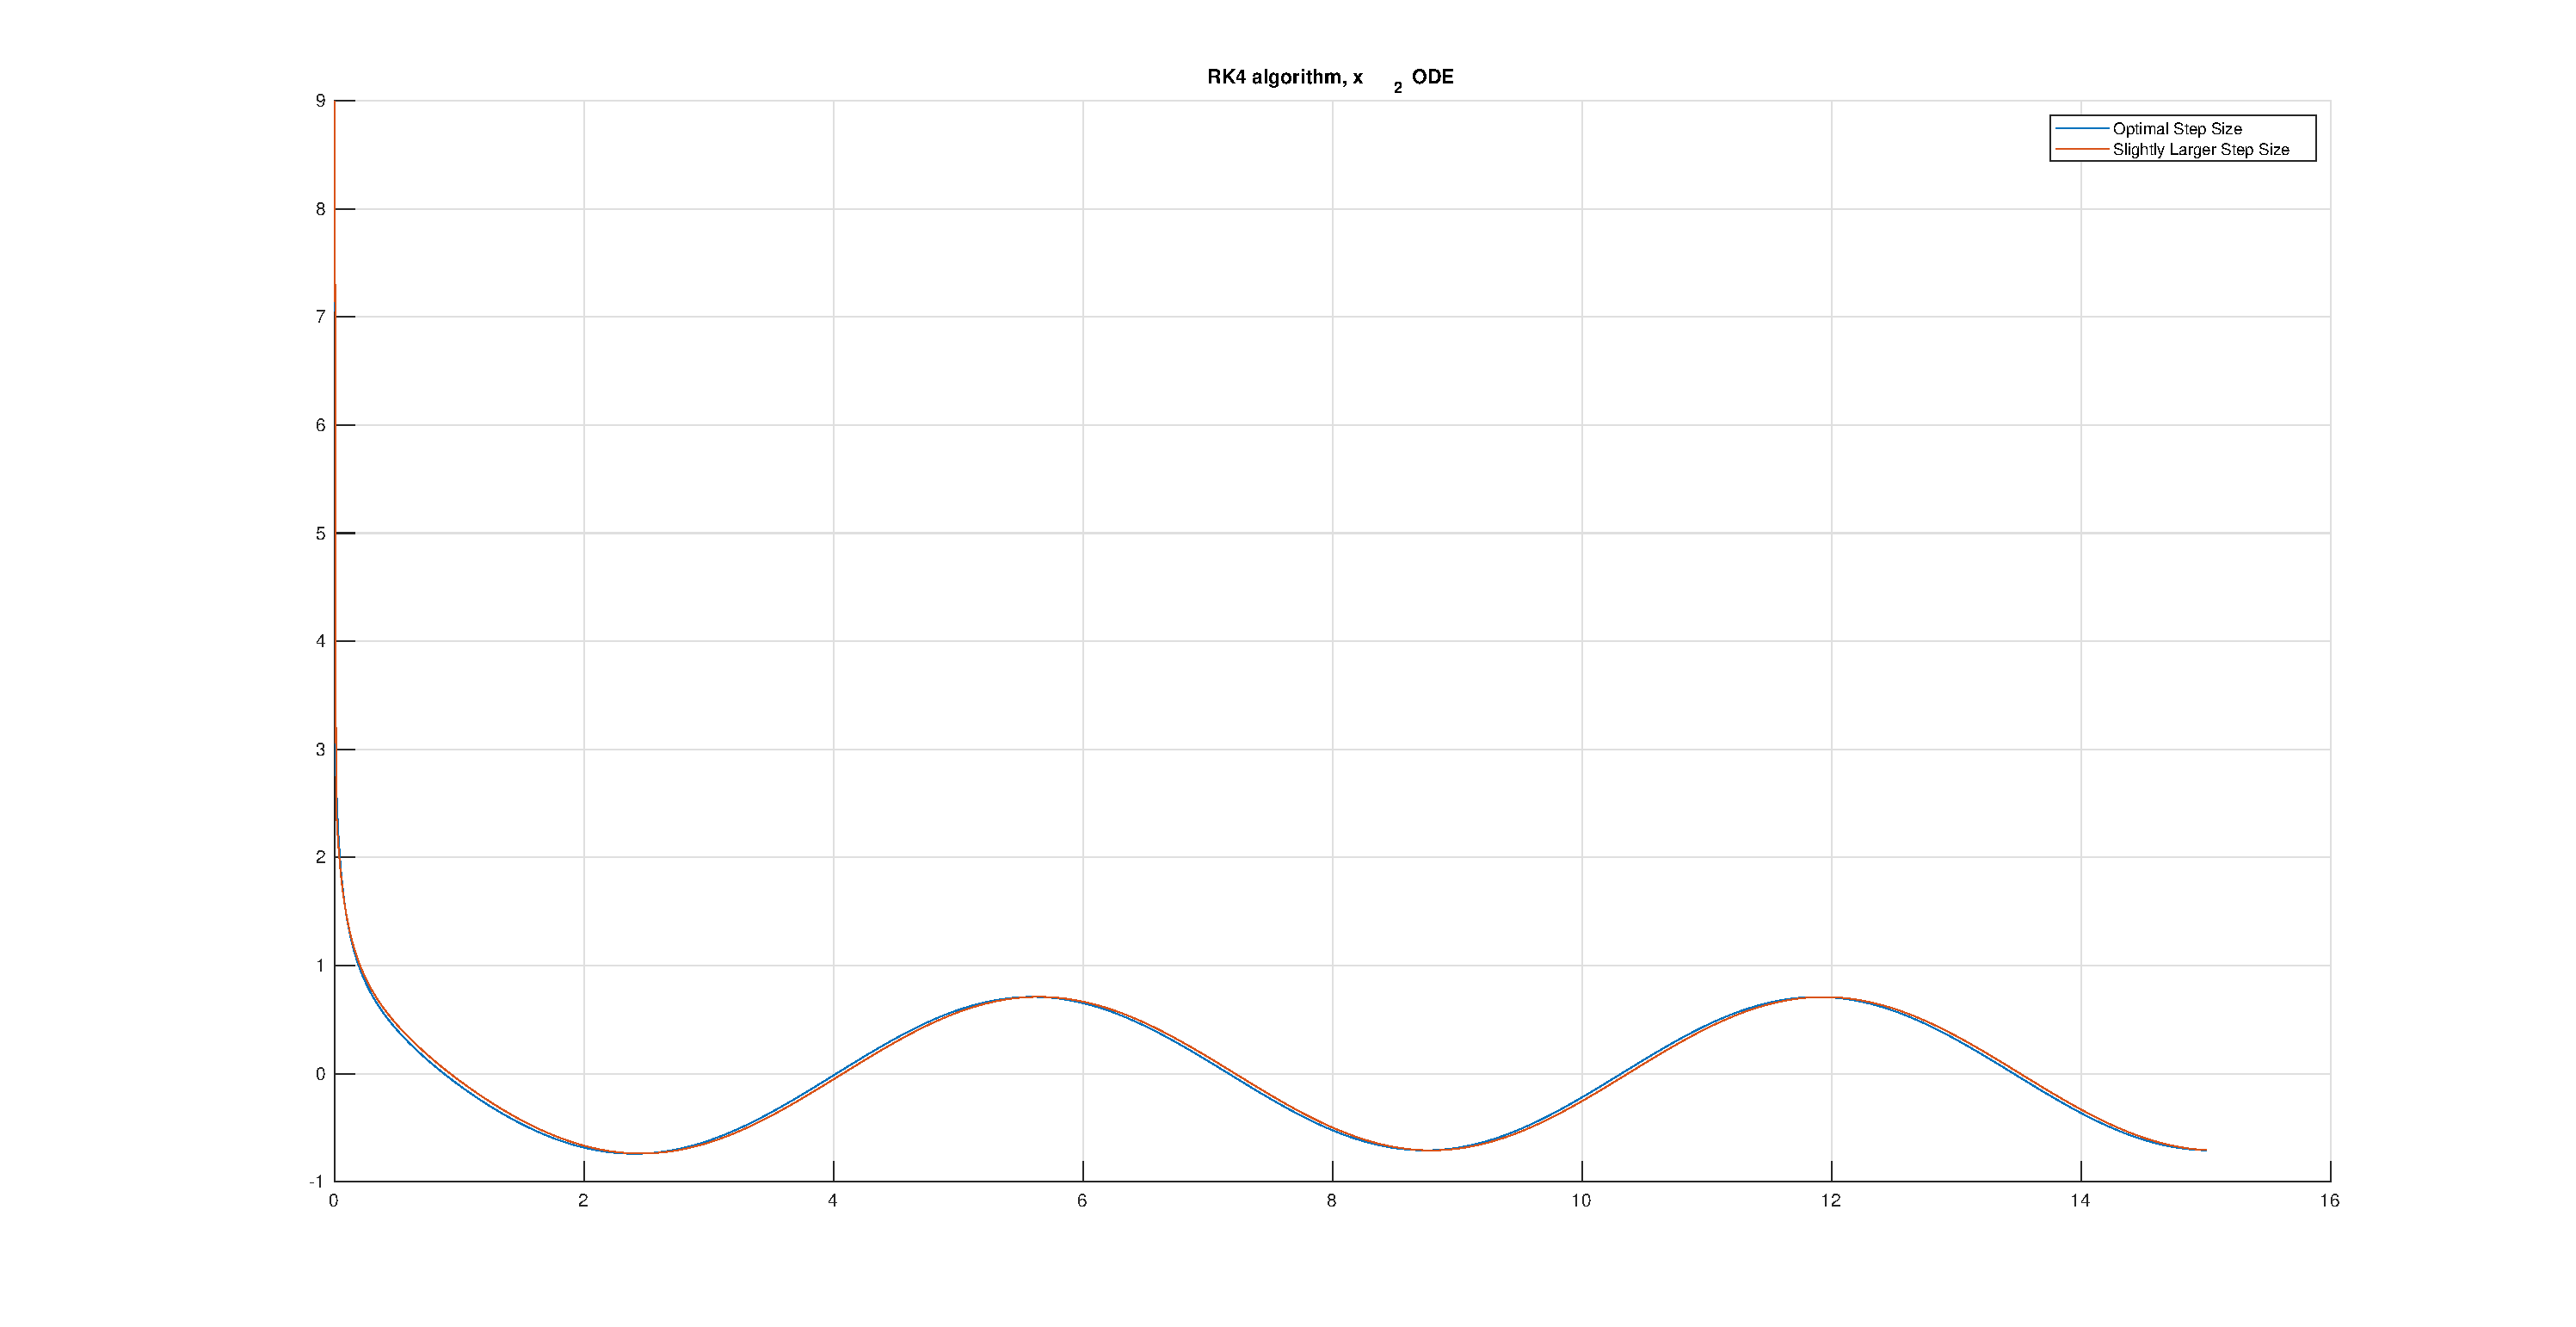
\includepdf[pages=-]{21-eps-converted-to.pdf}
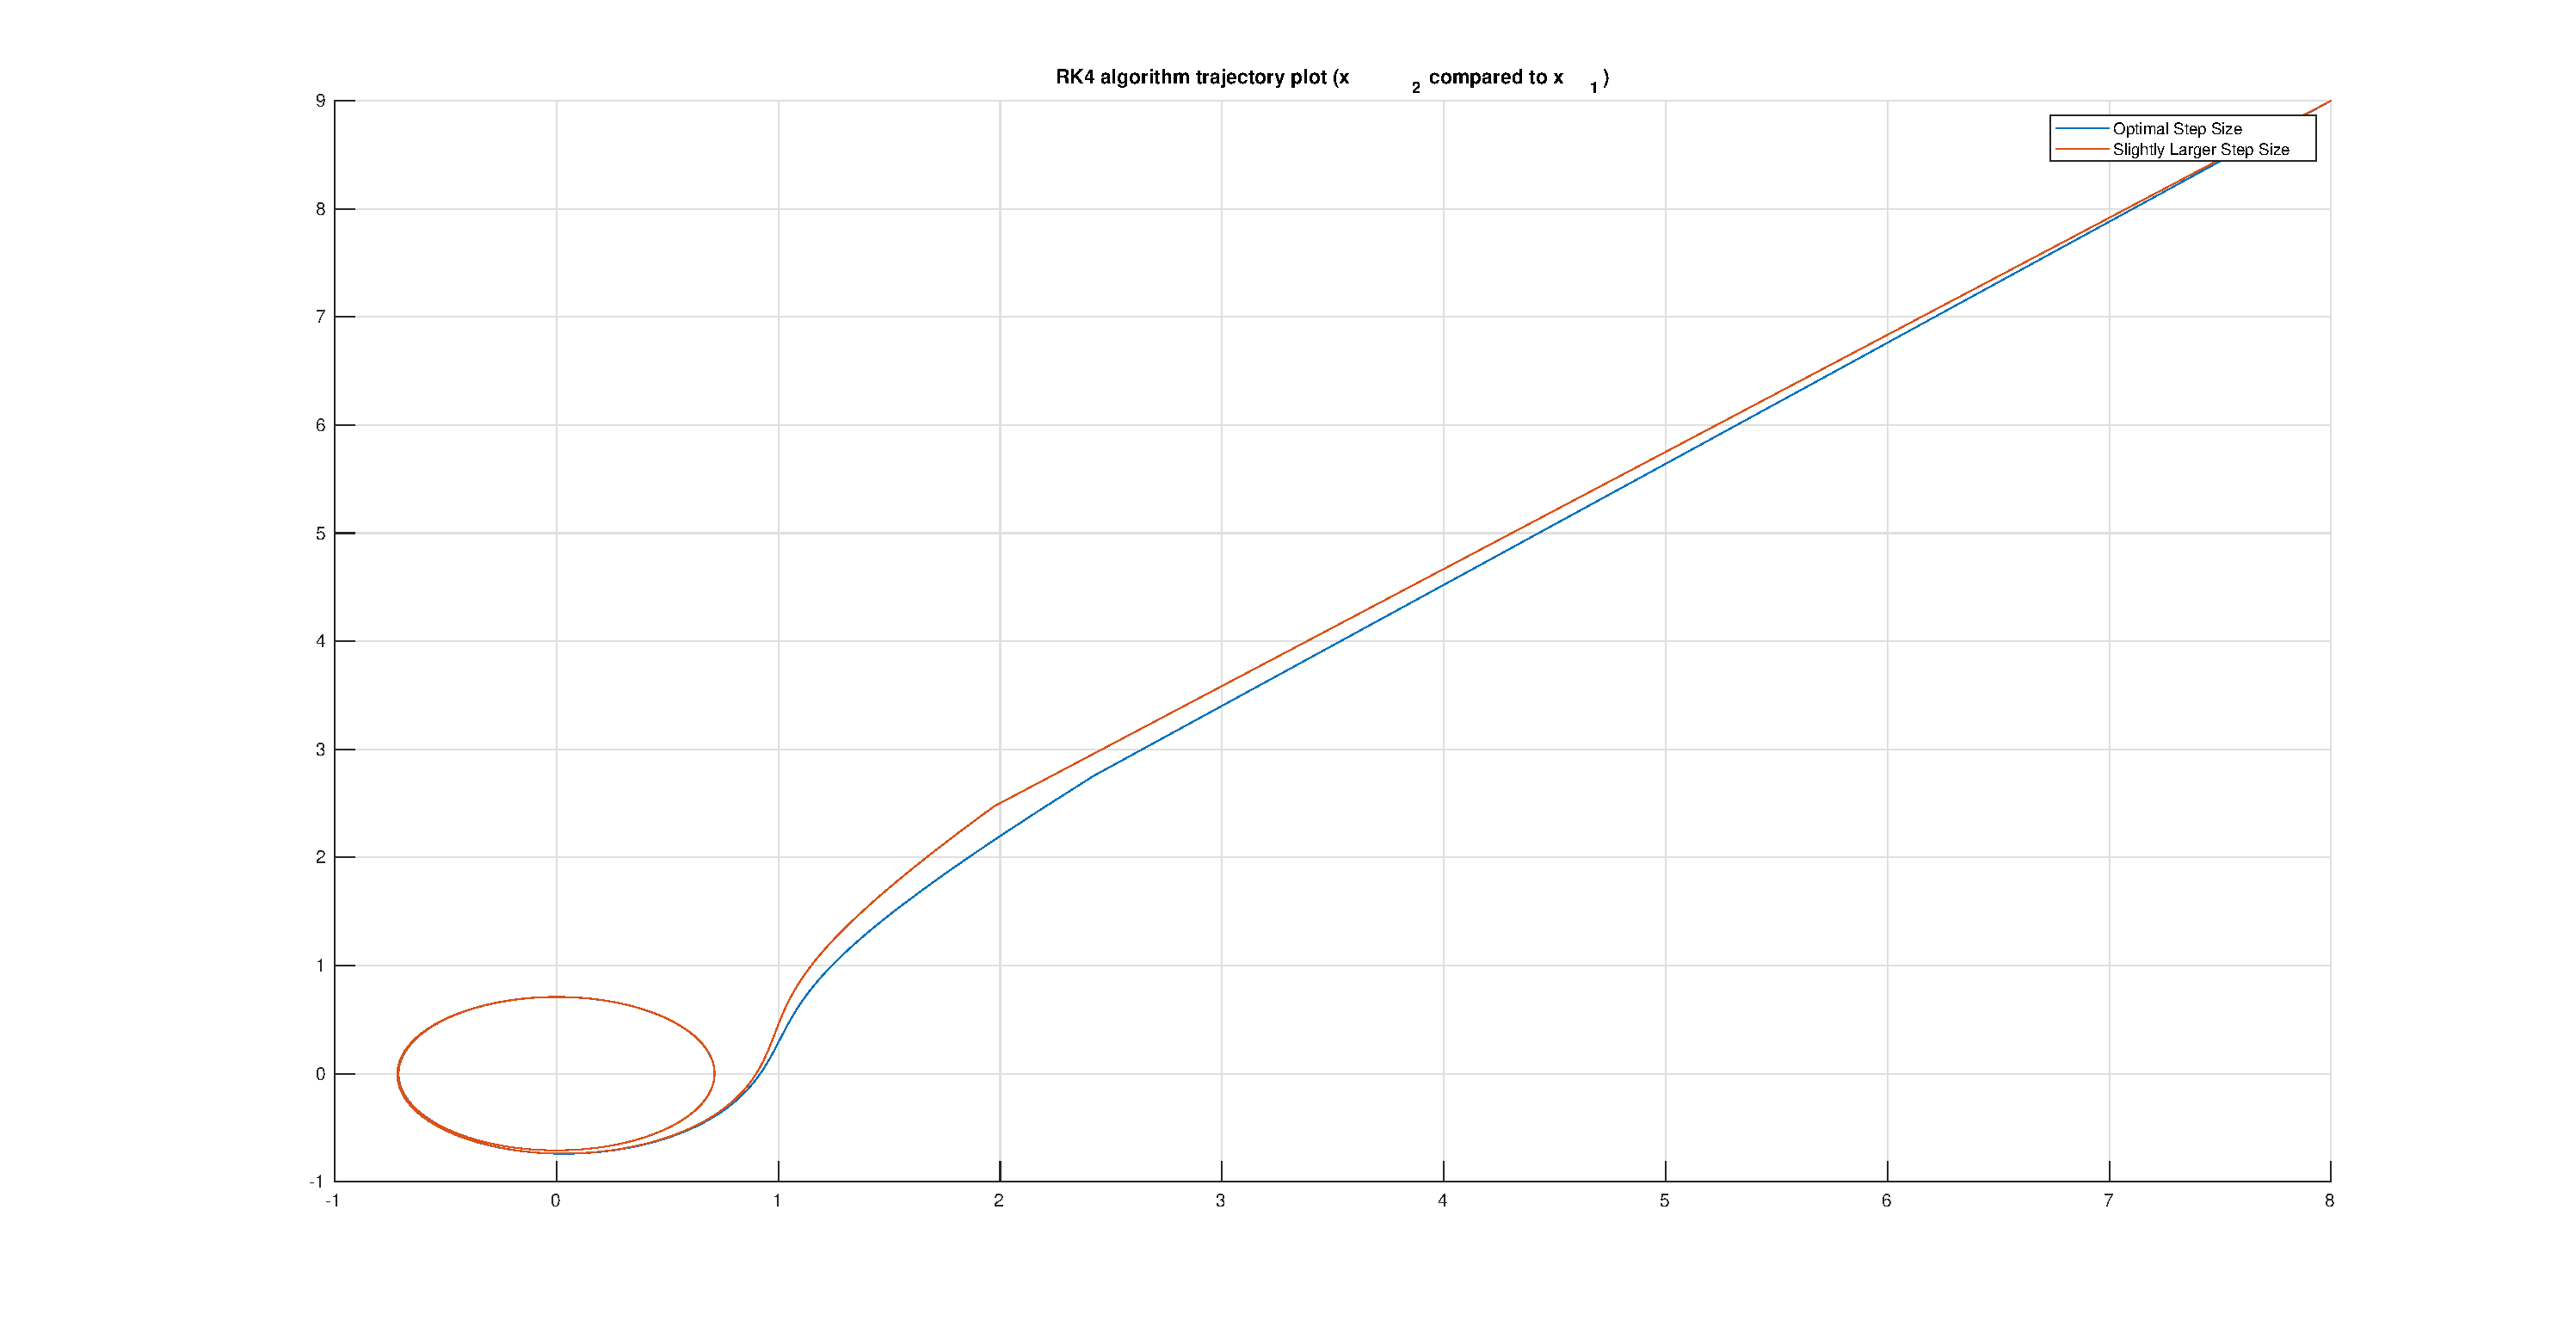
\includepdf[pages=-]{22-eps-converted-to.pdf}
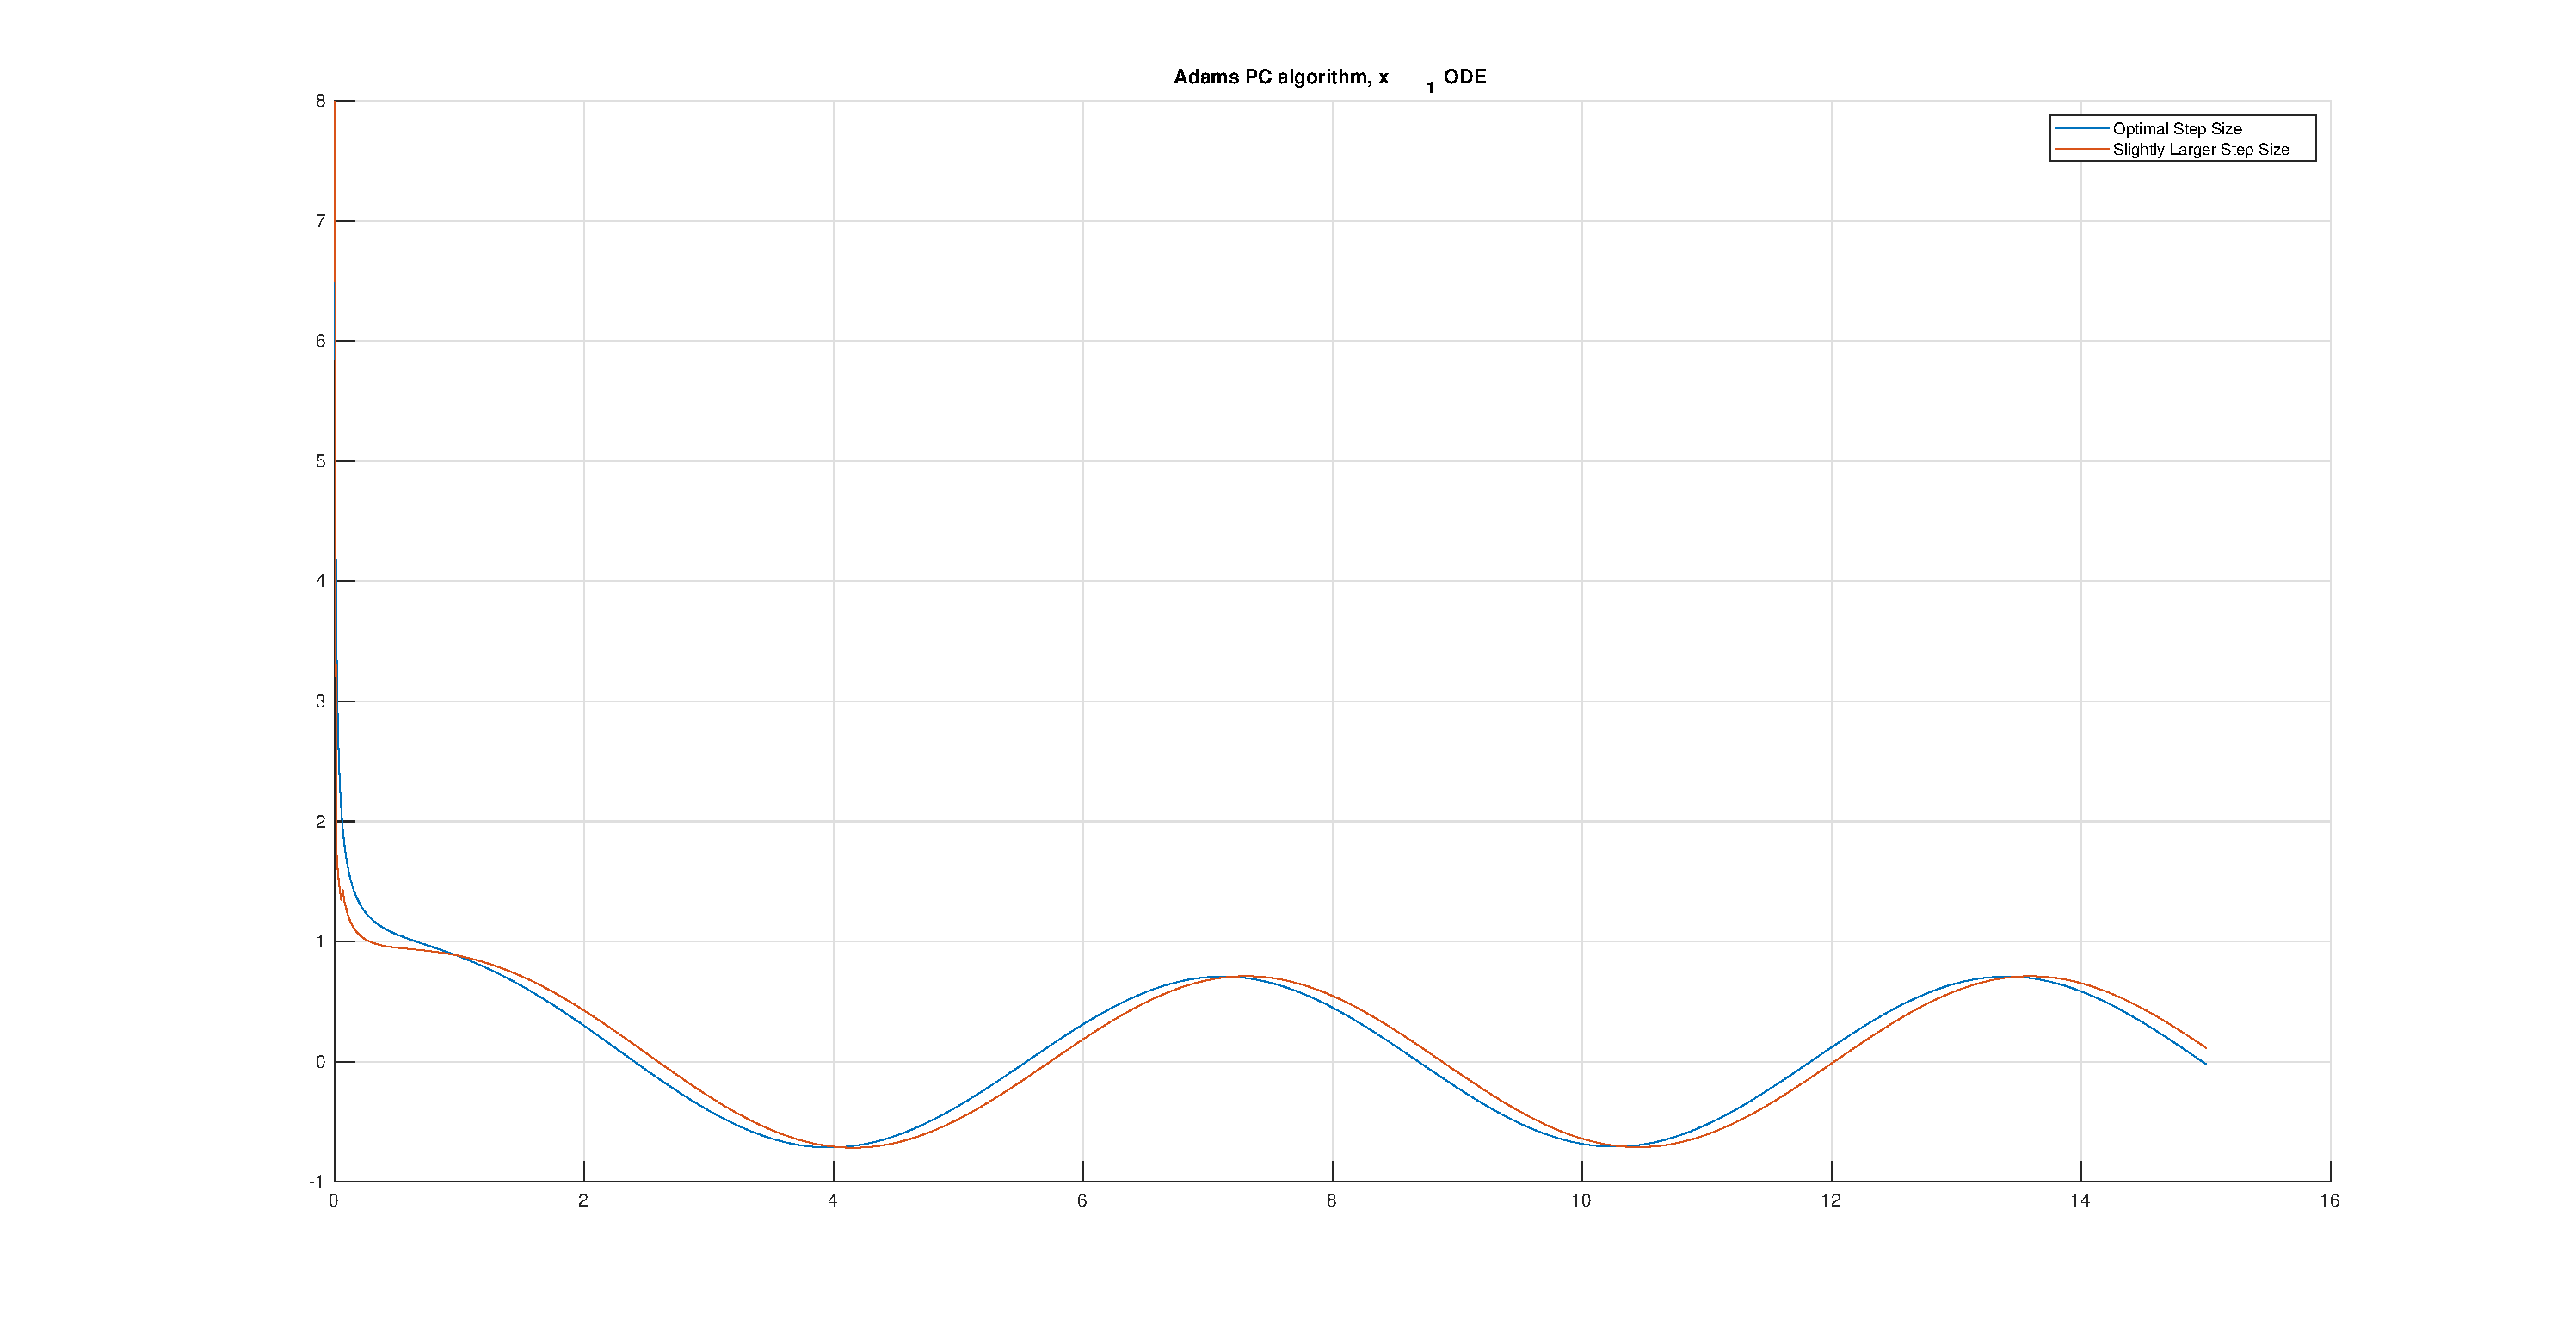
\includepdf[pages=-]{23-eps-converted-to.pdf}
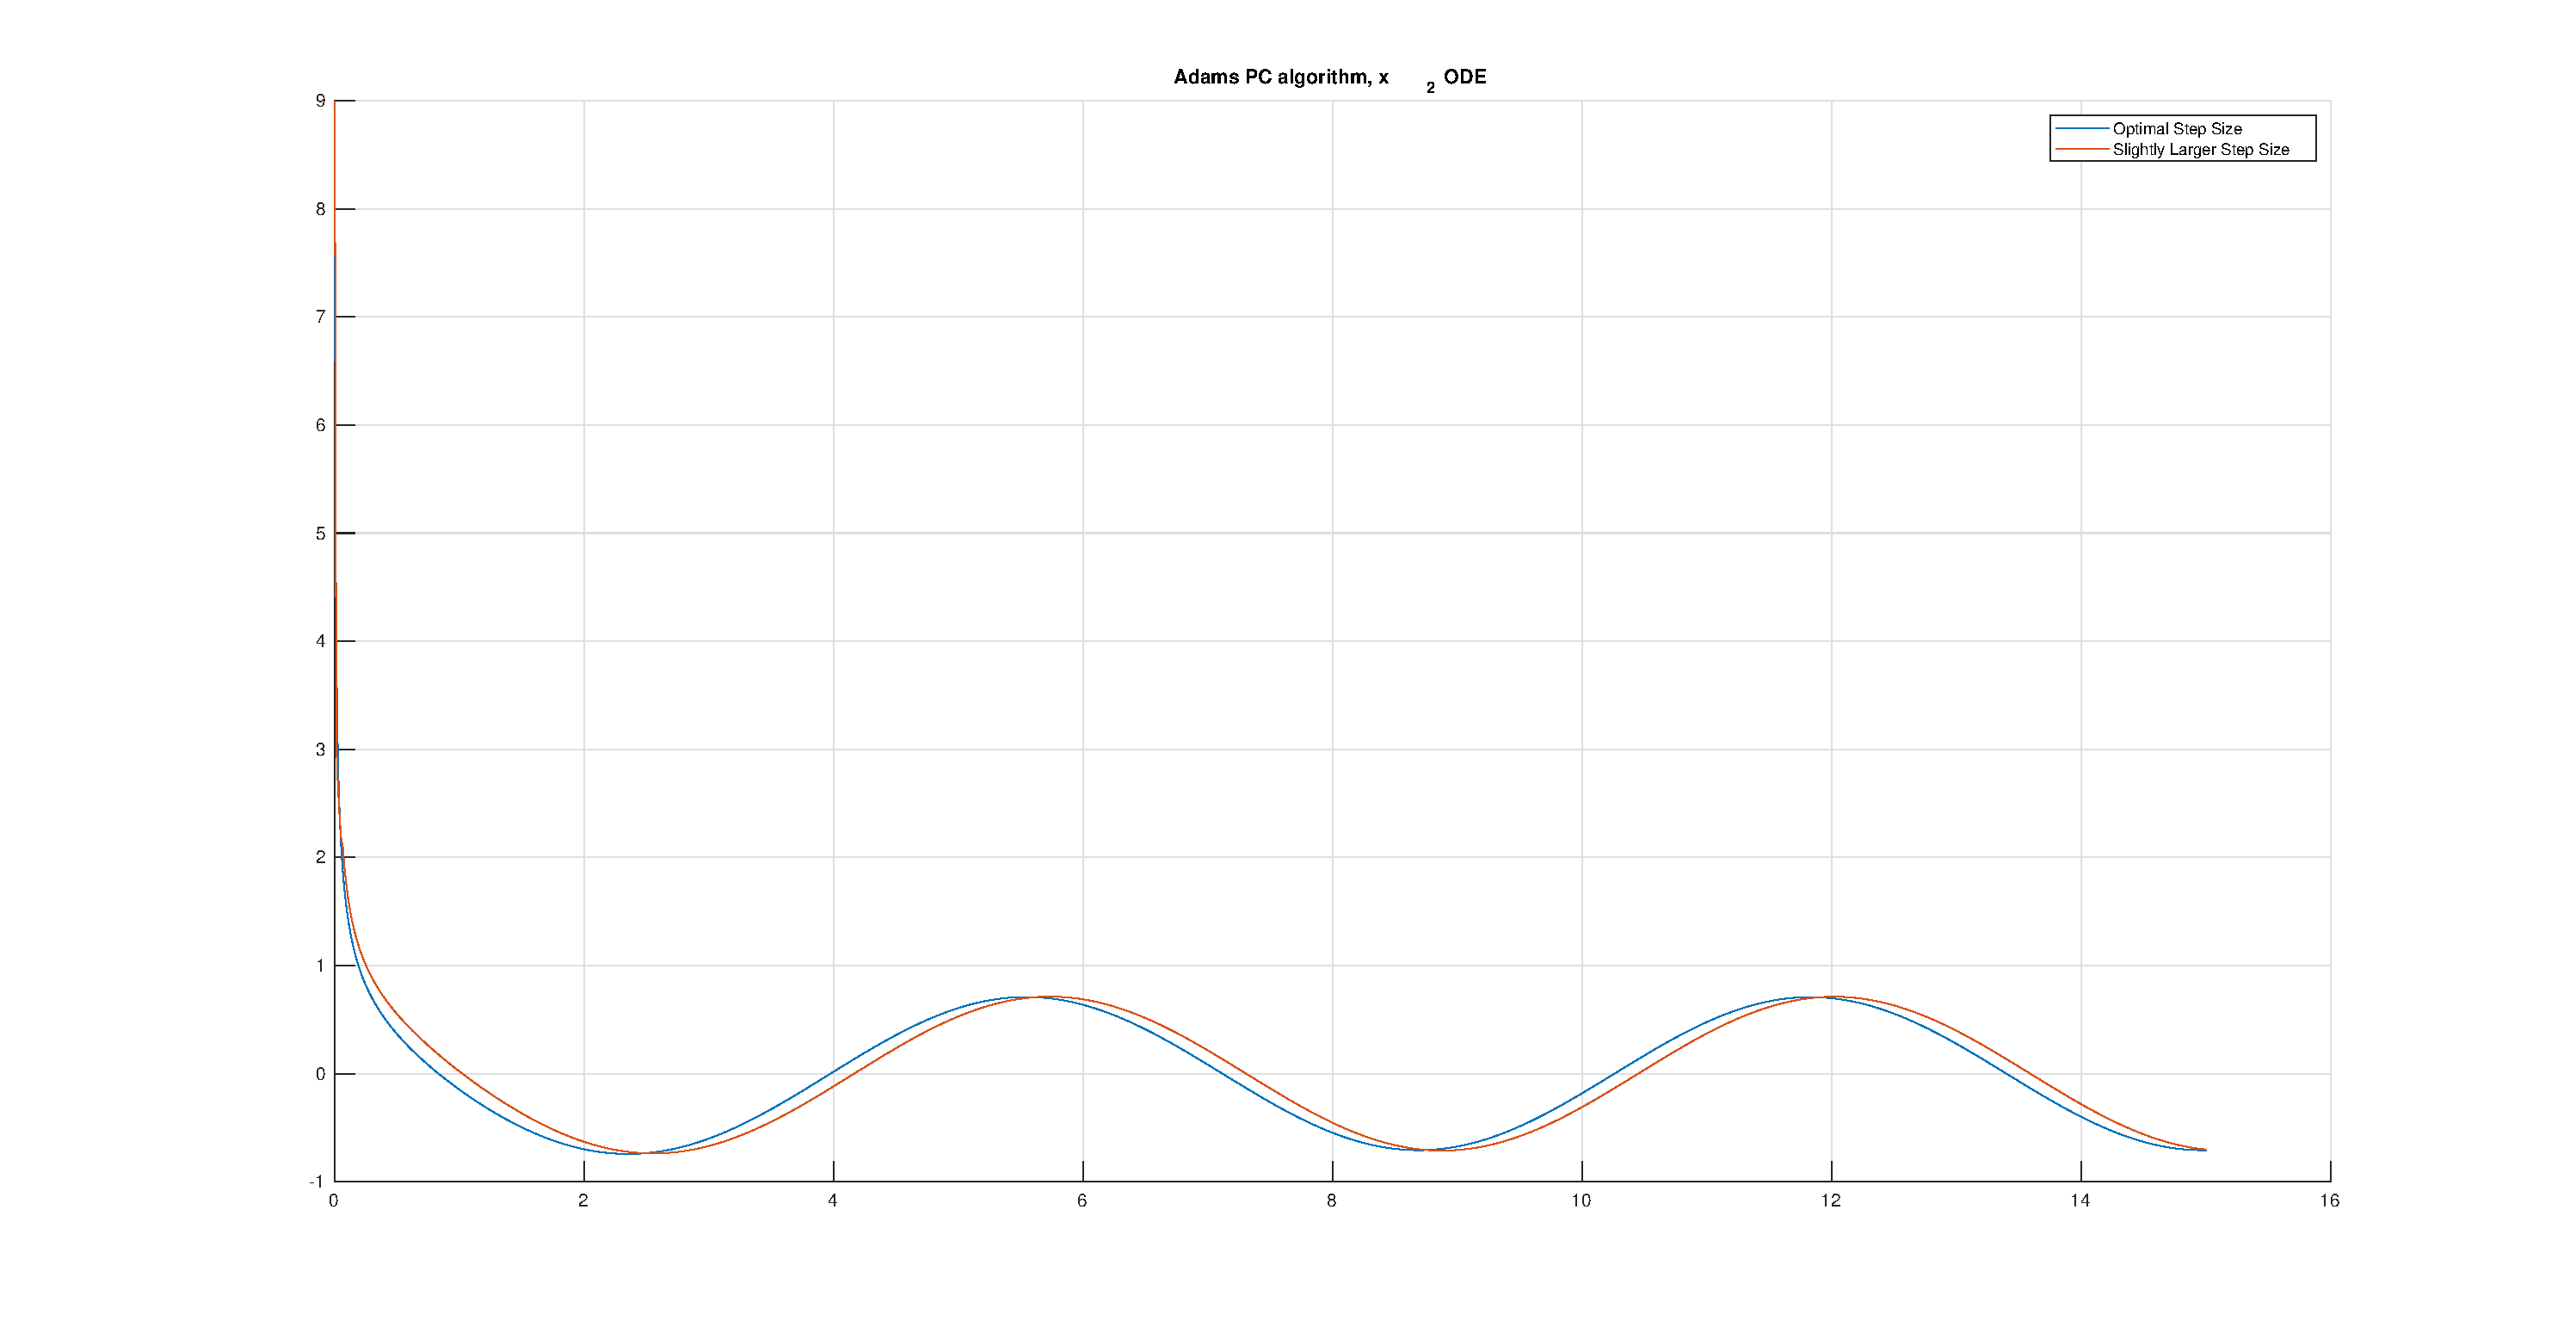
\includepdf[pages=-]{24-eps-converted-to.pdf}
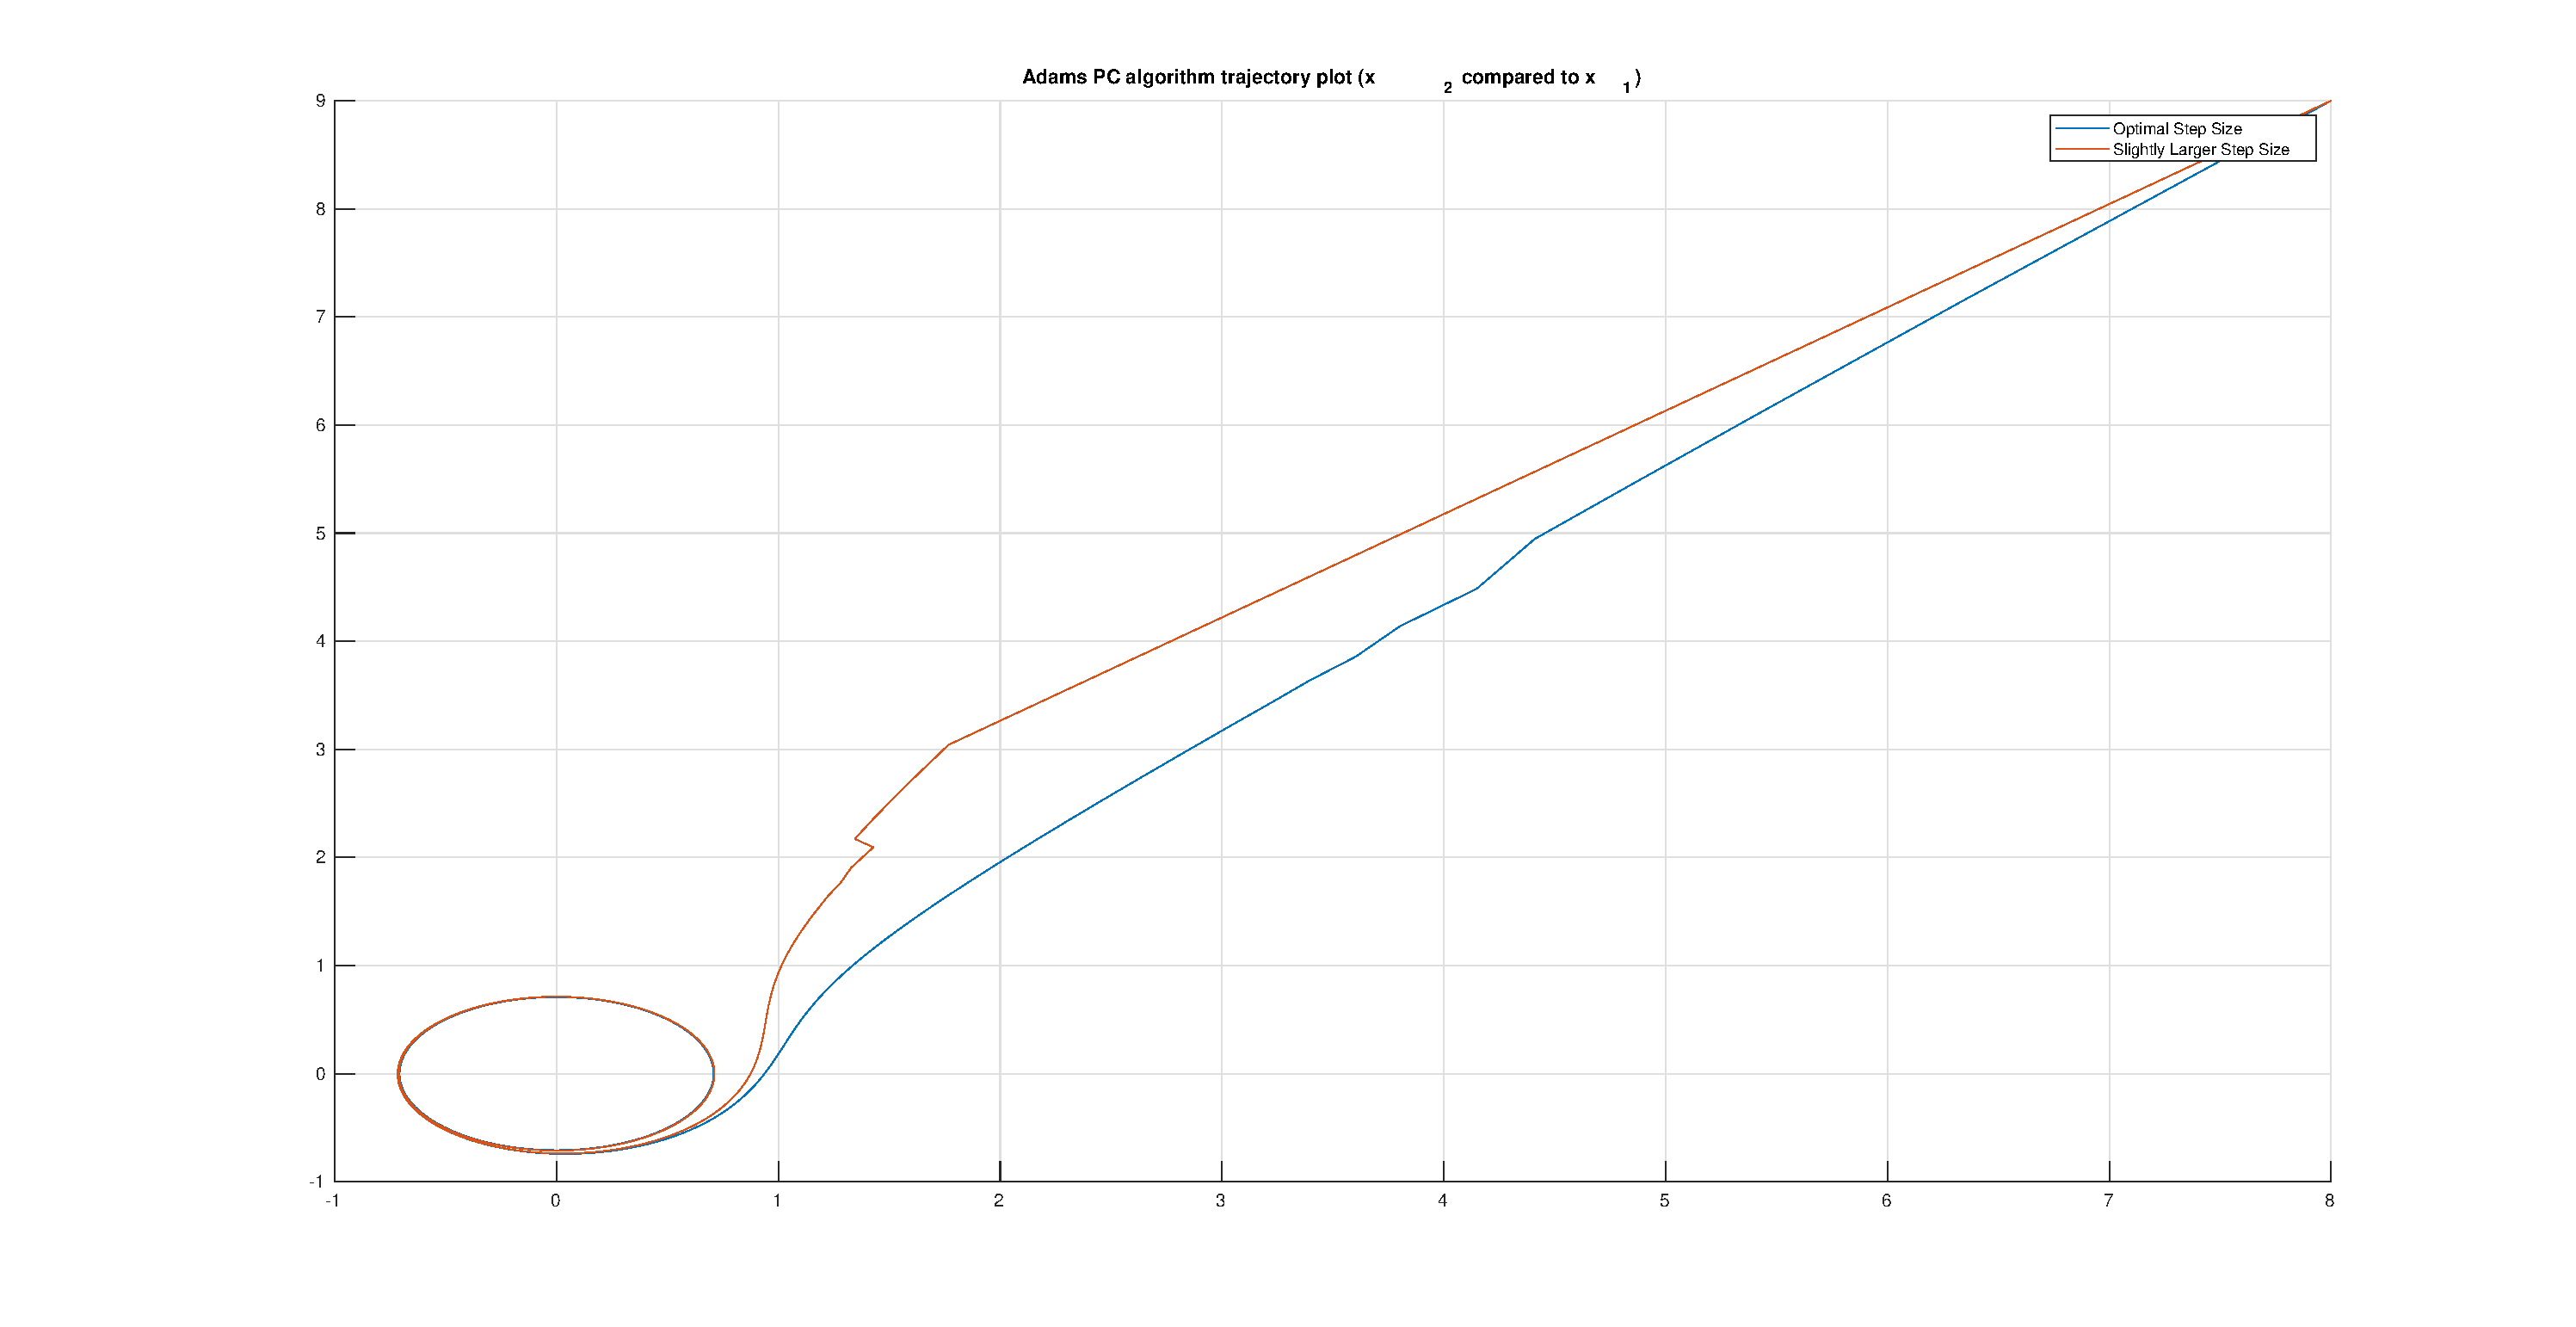
\includepdf[pages=-]{25-eps-converted-to.pdf}
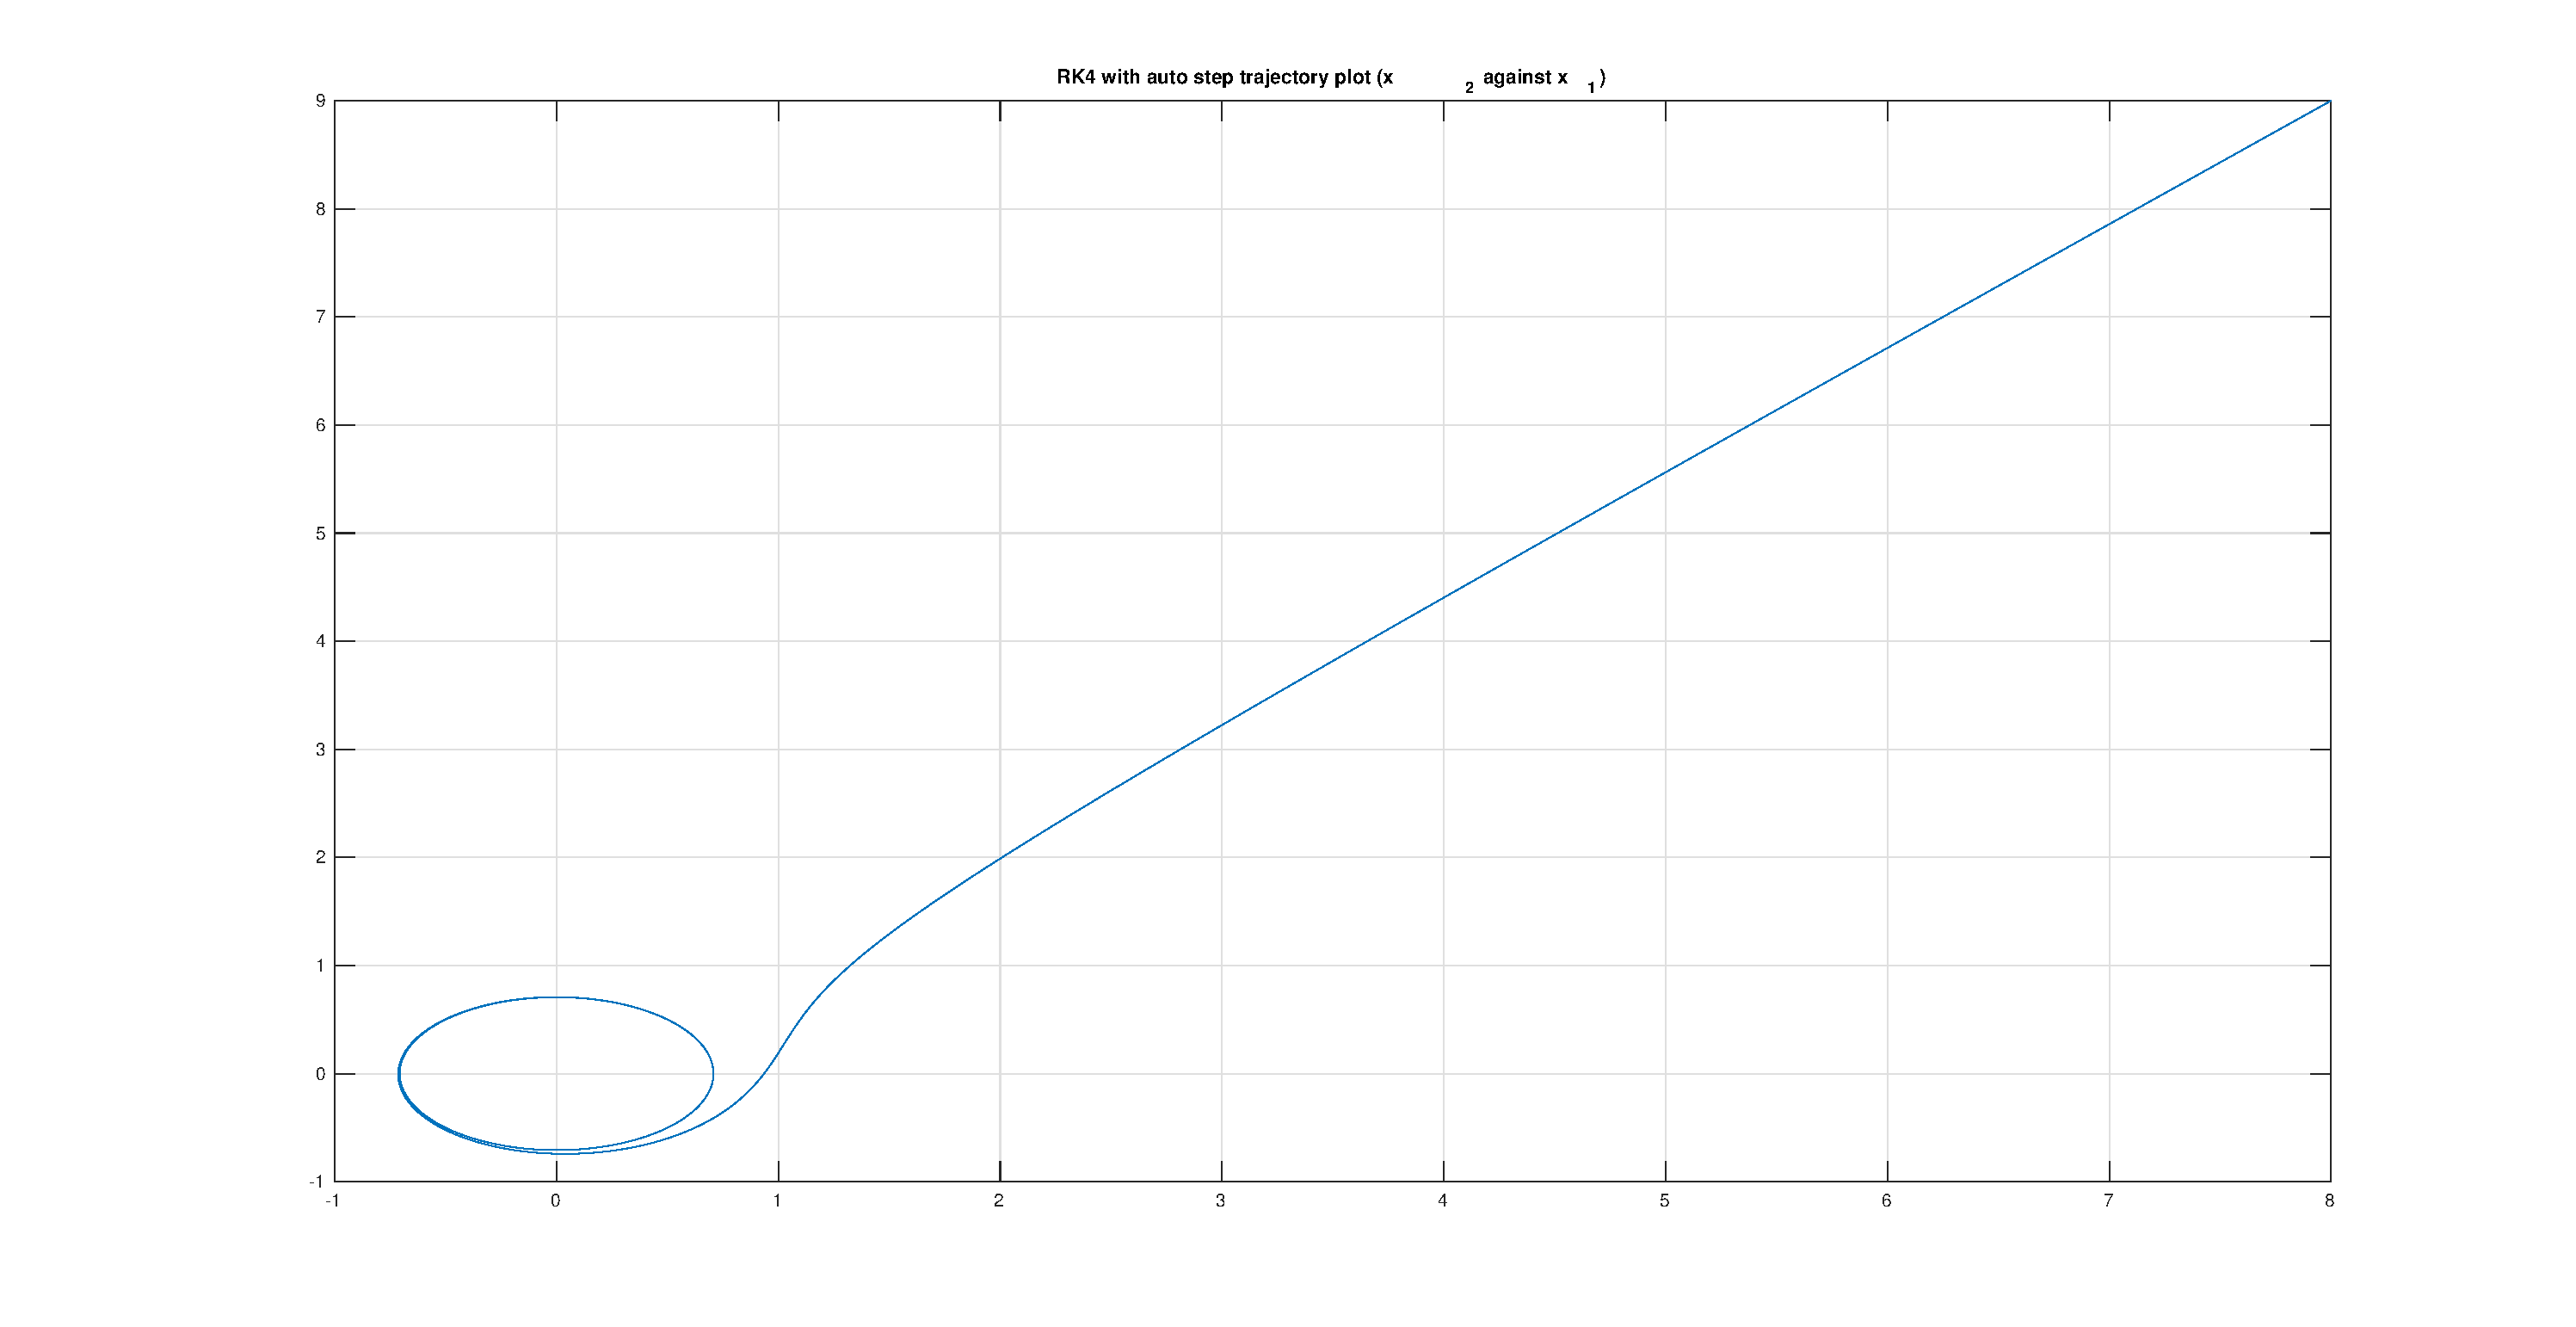
\includepdf[pages=-]{26-eps-converted-to.pdf}
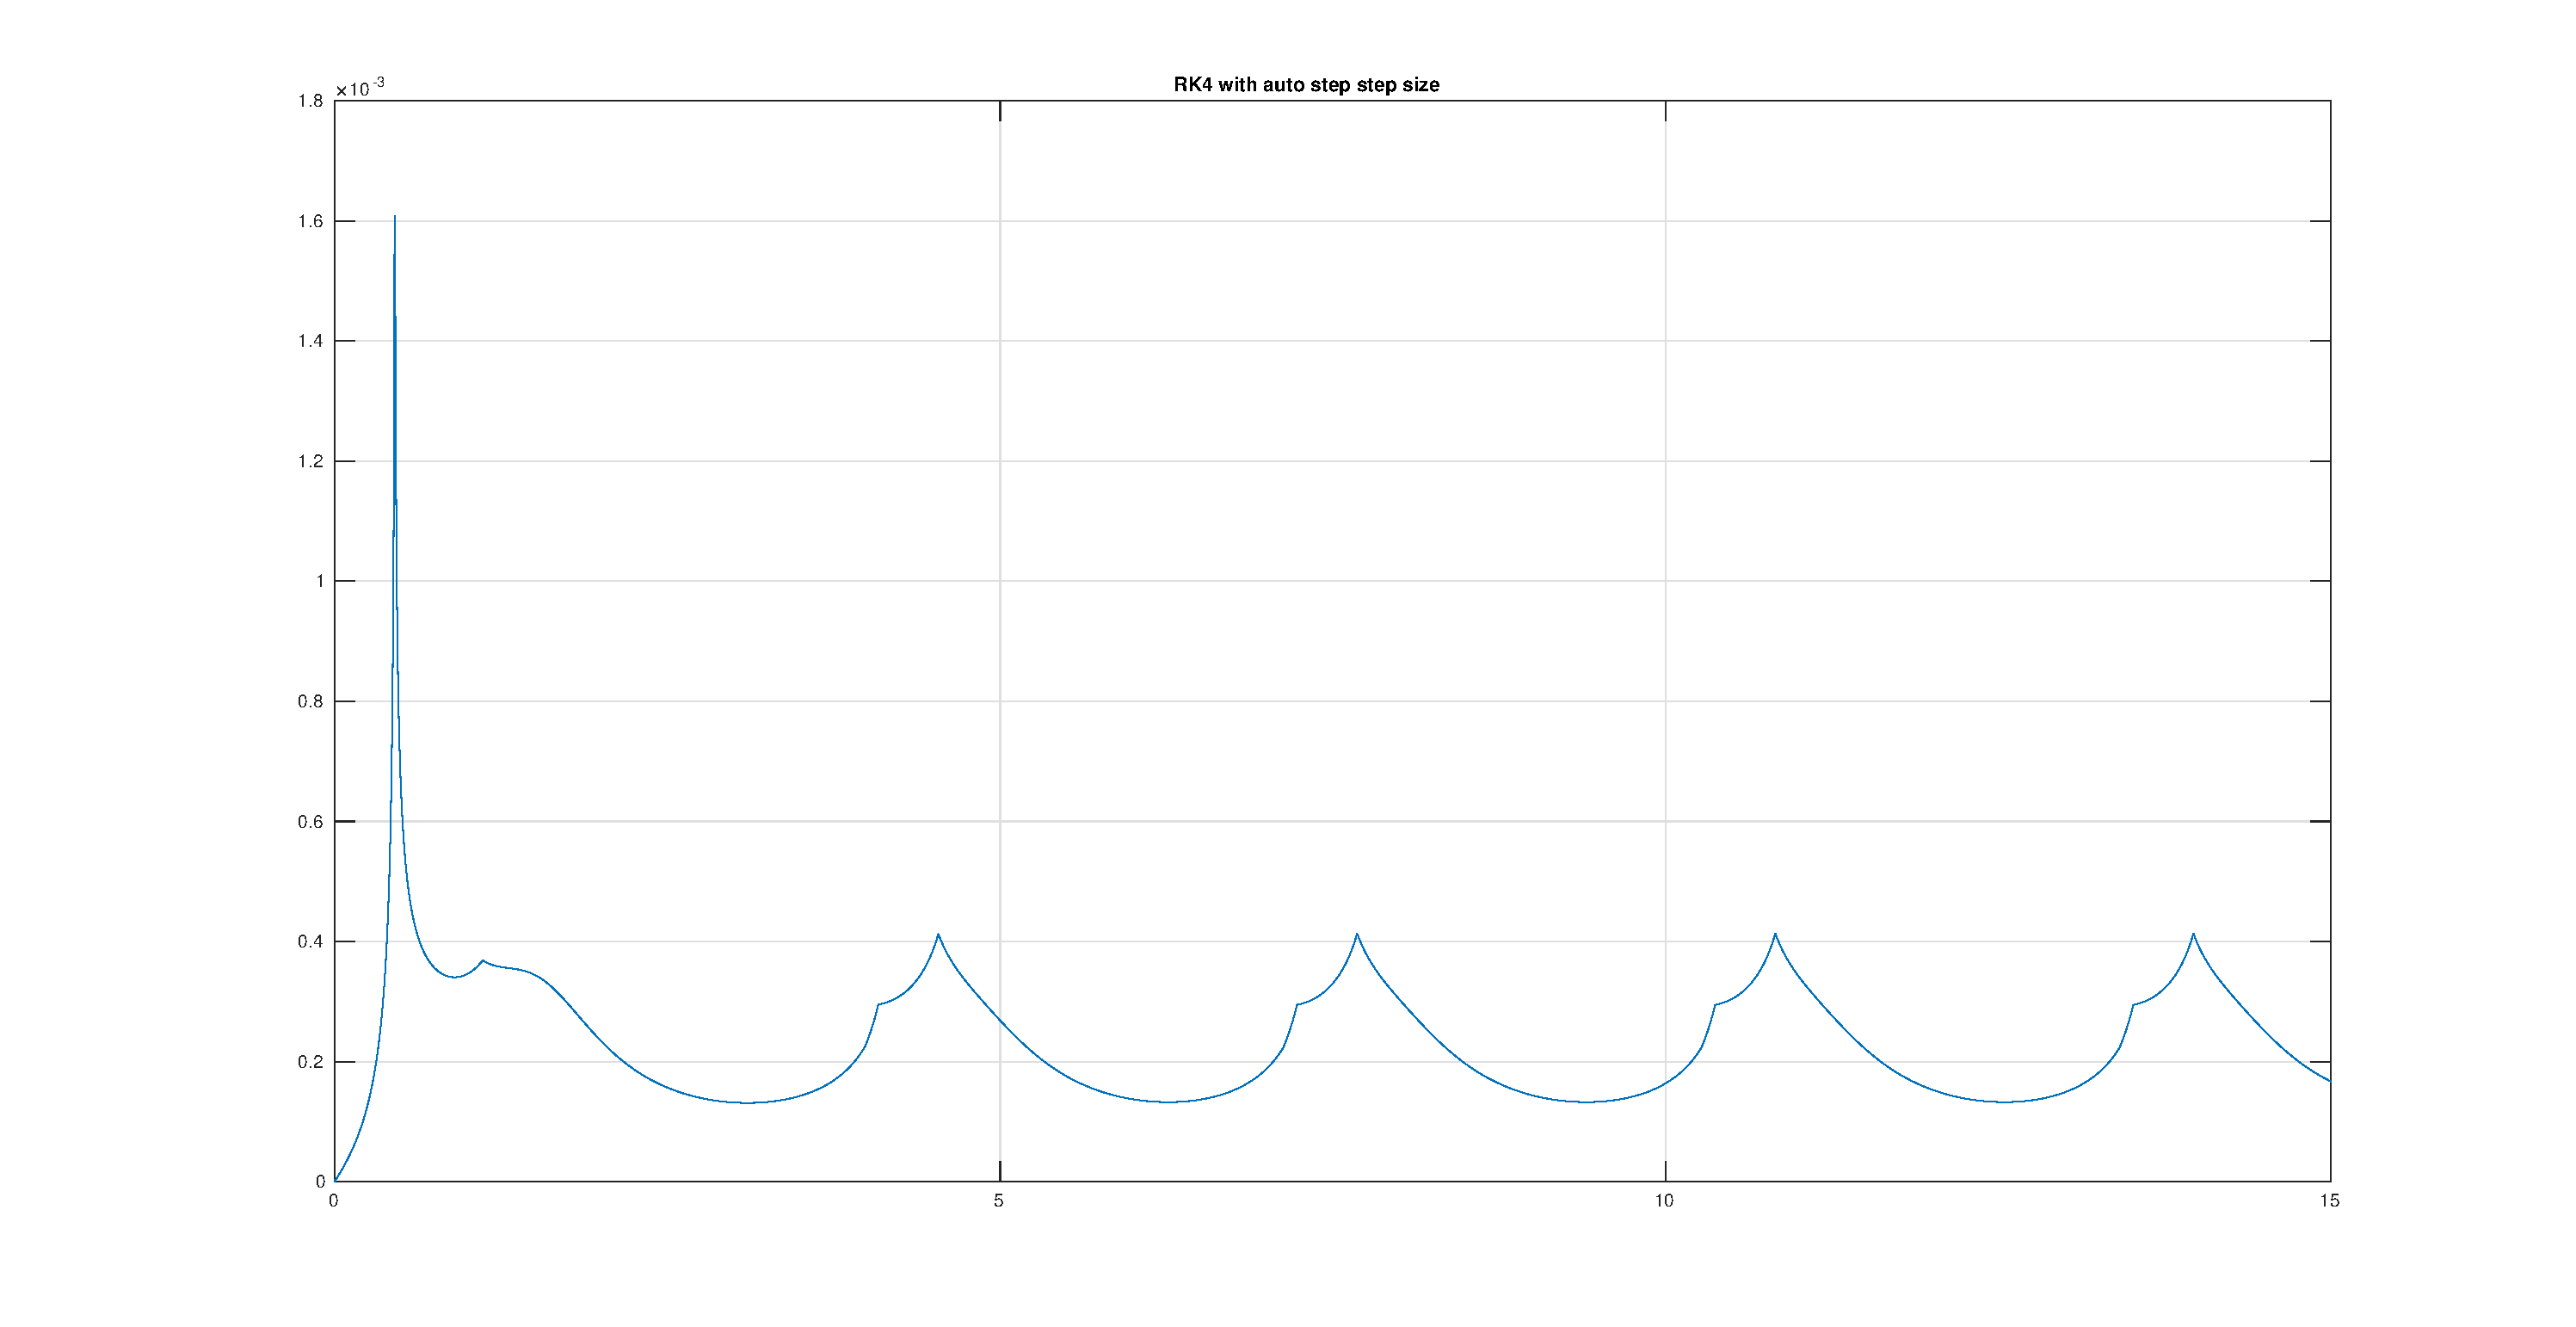
\includepdf[pages=-]{27-eps-converted-to.pdf}
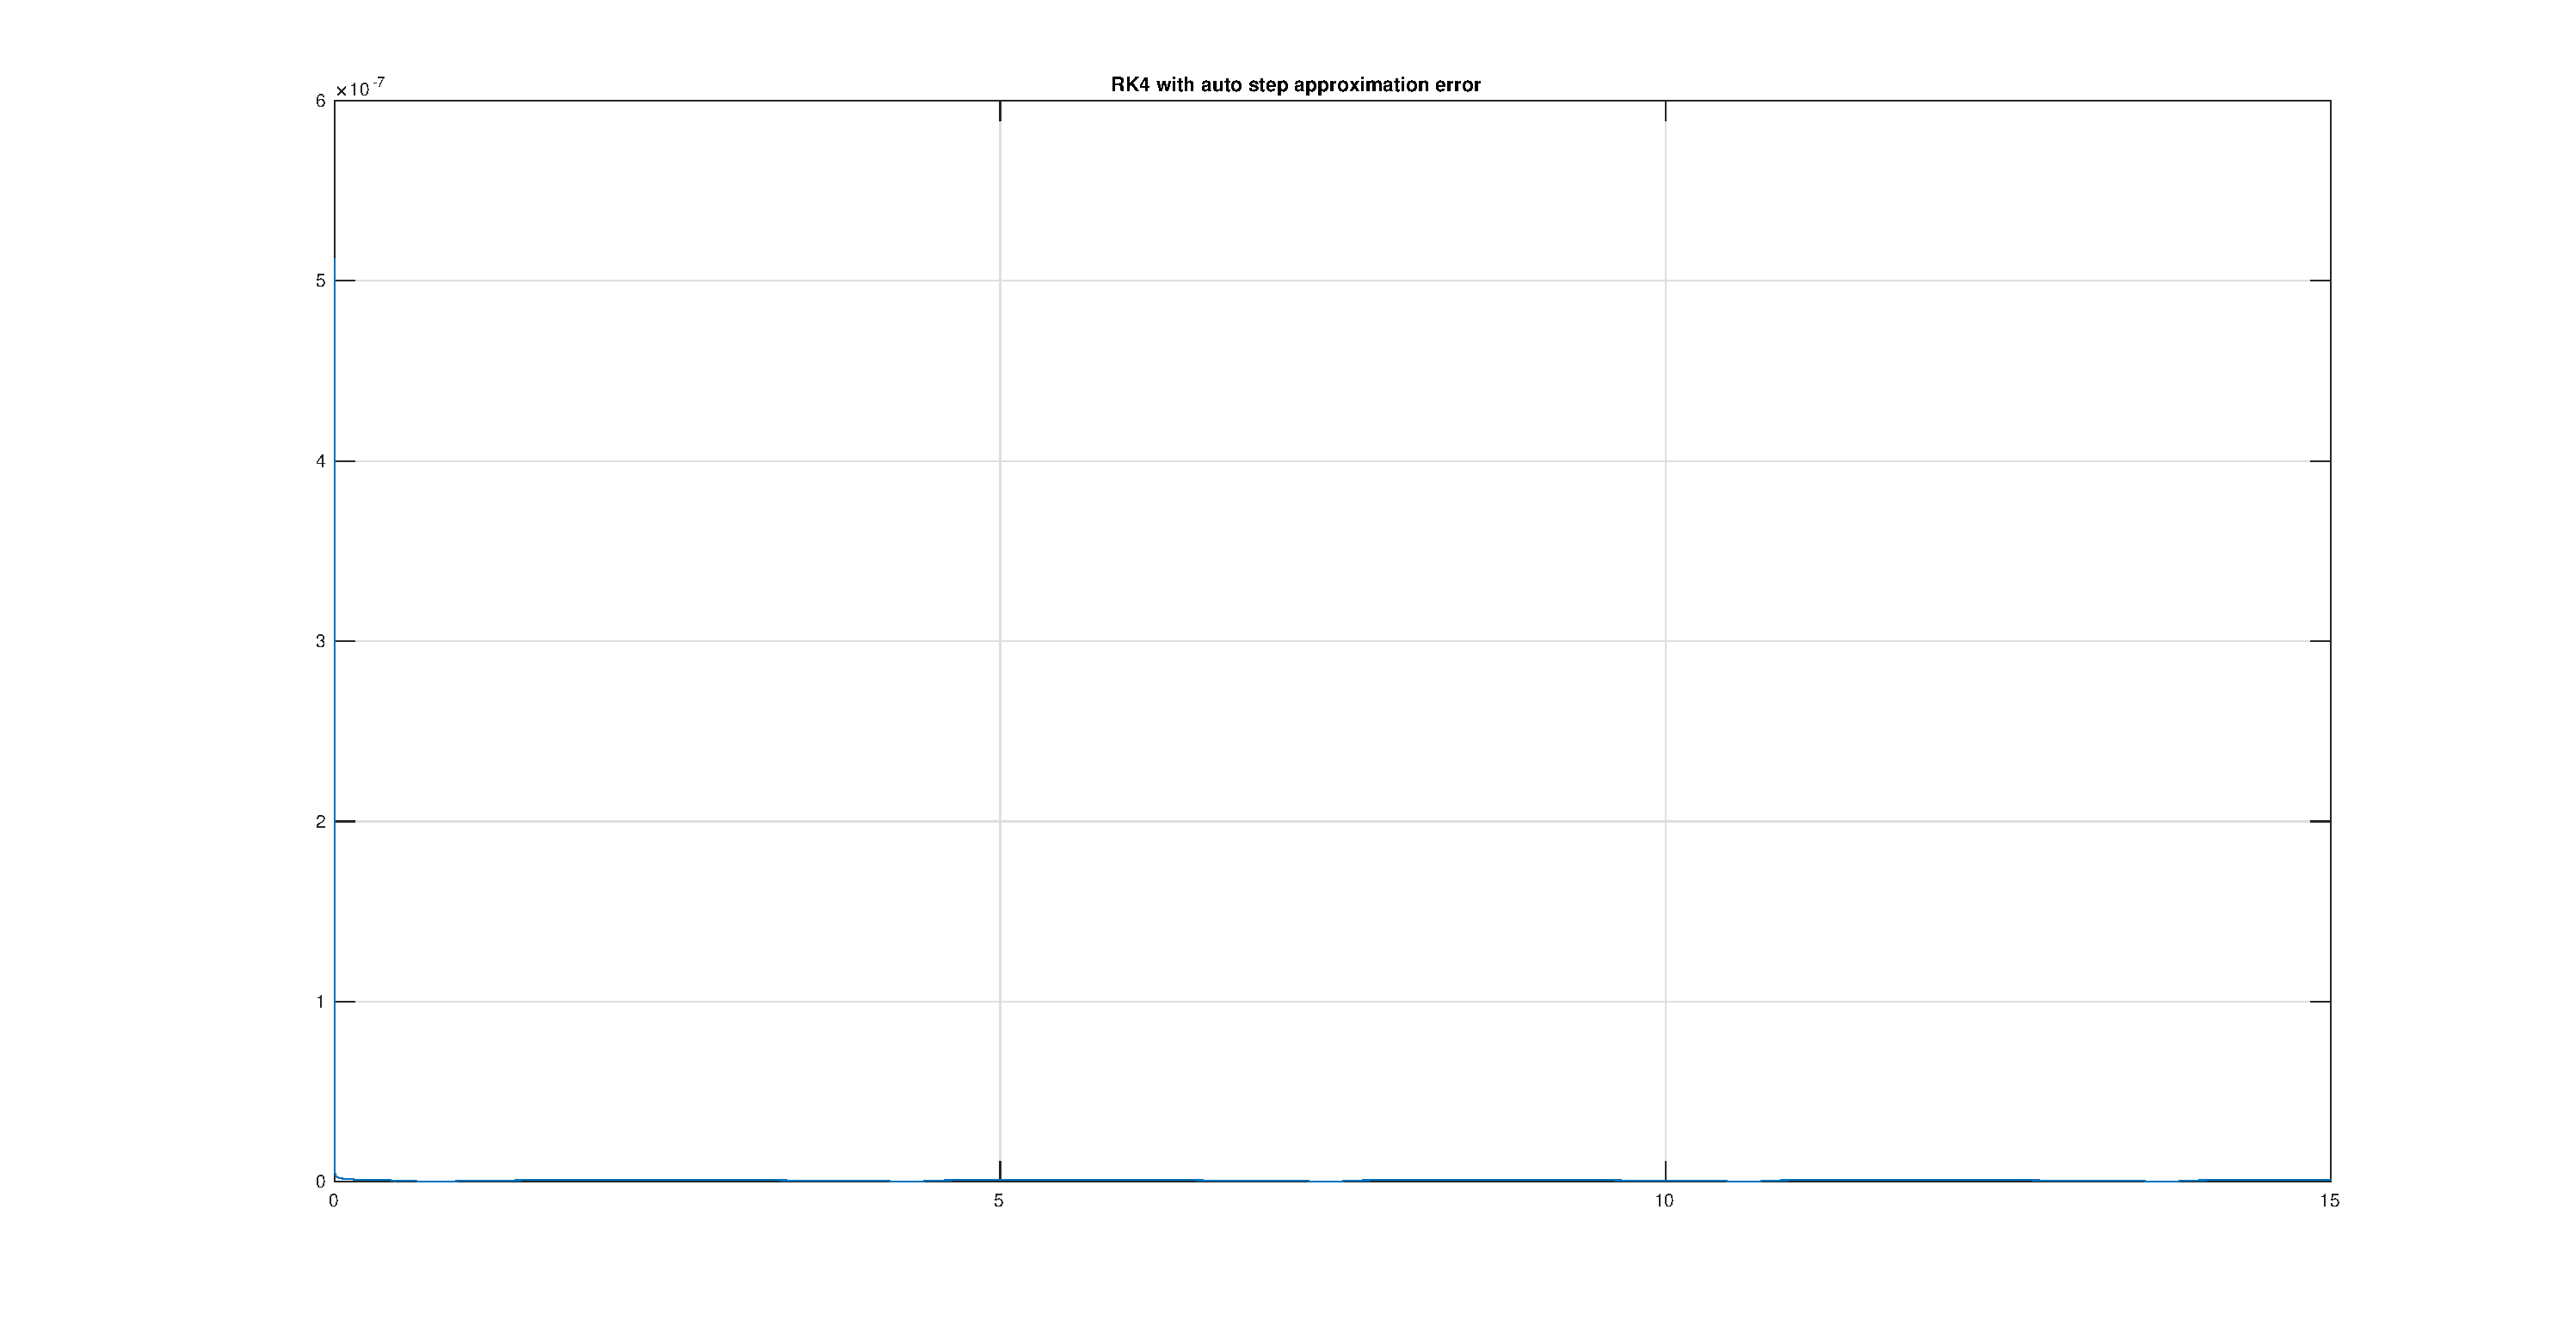
\includepdf[pages=-]{28-eps-converted-to.pdf}
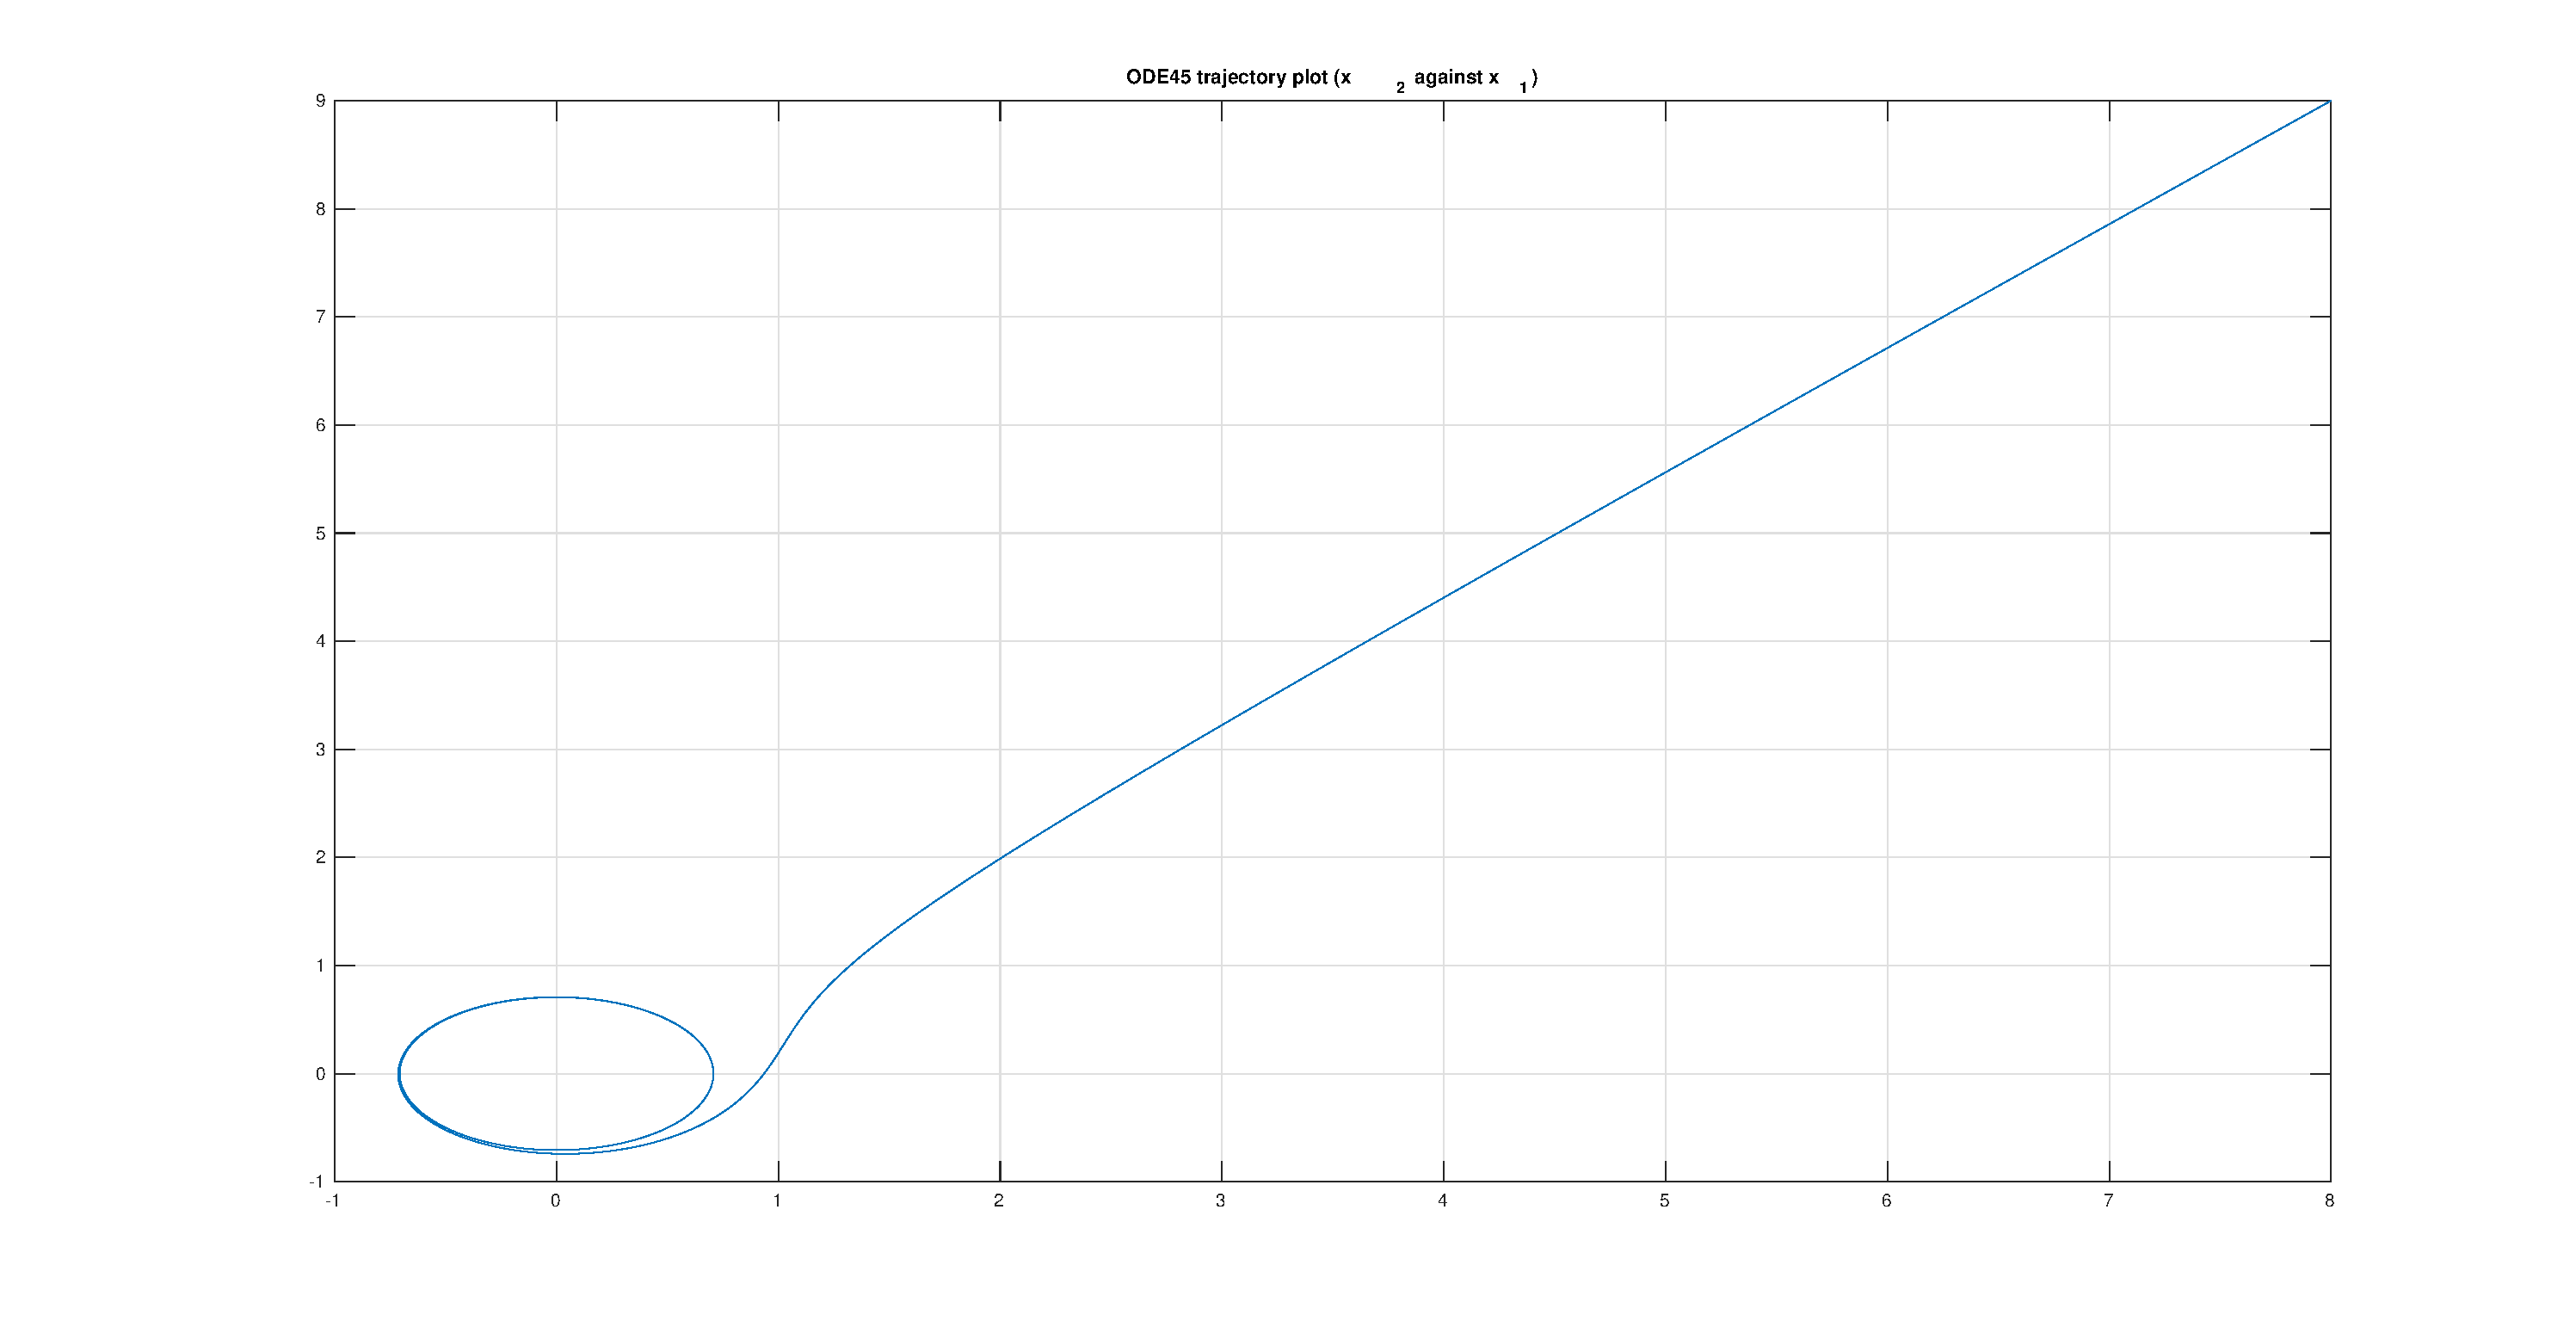
\includepdf[pages=-]{29-eps-converted-to.pdf}

\section{Discussion of results}
As we can see using RK4 algorithm with auto step size results in best solutions error-wise, trajectory plot is almost the same as the one generated by matlab function. Especially graph of step approximation error for RK4 auto step algorithm looks very good with errors as low as $10^{-7}$. Adam PC method on the other hand suffers from bigger accuarcy loss though the results are still satisfactory while requiring much less work on the coding part.

\chapter{Code appendix}

\section{functionDataPoints.m}
\subsection{functionDataPoints}
\begin{simplechar}
\begin{lstlisting}
function dataPoints = functionDataPoints()
    dataPoints = (-5:5)';
    dataPoints(:, 2) = [
        -6.5743
        0.9765
        3.1026
        1.8572
        1.3165
        -0.6144
        0.1032
        0.3729
        2.5327
        7.3857
        9.4892
    ];
end
\end{lstlisting}
\end{simplechar}

\section{task1.m}
\subsection{task1}
\begin{simplechar}
\begin{lstlisting}
function task1(polynomialDegree)
    for currentPolynomialDegree = 0 : polynomialDegree
        dataPoints = functionDataPoints();
        % obtain LSPSolutions of approximating polynomial
        [LSPSolutions, error, conditionNumber] = approximate(dataPoints, currentPolynomialDegree);
        displayInfo(currentPolynomialDegree, error, conditionNumber);
        plotGraph(currentPolynomialDegree, dataPoints, LSPSolutions)
    end
end
\end{lstlisting}
\end{simplechar}

\subsection{displayInfo}
\begin{simplechar}
\begin{lstlisting}
function displayInfo(currentPolynomialDegree, error, conditionNumber)
    disp("Current Polynomial Degree:");
    disp(currentPolynomialDegree);
    disp("Error: ");
    disp(error);
    disp("Condition number of Gram's Matrix: ");
    disp(conditionNumber);
end
\end{lstlisting}
\end{simplechar}

\subsection{plotGraph}
\begin{simplechar}
\begin{lstlisting}
function plotGraph(currentPolynomialDegree, dataPoints, LSPSolutions)
    figure;
    grid on;
    hold on;
    plotDataPoints(currentPolynomialDegree, dataPoints);
    plotApproximation(dataPoints, LSPSolutions);
    hold off;
end
\end{lstlisting}
\end{simplechar}

\subsection{plotDataPoints}
\begin{simplechar}
\begin{lstlisting}
function plotDataPoints(currentPolynomialDegree, dataPoints)
    title(['Polynomial approximation of the funtion using: ', num2str(currentPolynomialDegree), ' degree']);
    scatter(dataPoints(:, 1), dataPoints(:, 2), 72, 'x');
end
\end{lstlisting}
\end{simplechar}

\subsection{plotApproximation}
\begin{simplechar}
\begin{lstlisting}
function plotApproximation(dataPoints, LSPSolutions)
    x = dataPoints(1):0.05:dataPoints(end, 1);
    y = valueApproximationAtx(LSPSolutions, x);
    plot(x, y);
end

\end{lstlisting}
\end{simplechar}

\subsection{approximate}
\begin{simplechar}
\begin{lstlisting}
% find the approximating polynomial of the given degree
function [LSPSolutions, error, conditionNumber] = approximate(dataPoints, polydeg)
    % initialize A matrix
    A = zeros(size(dataPoints, 1), polydeg + 1);

    A = calculateACells(dataPoints, A);
    LSPSolutions = solveLSP(A, dataPoints);

    % Calculate error of solution
    error = norm(dataPoints(:, 2) - A * LSPSolutions);
    % Calculate condition number of Gram's matrix
    GramsMatrix = A' * A;
    conditionNumber = cond(GramsMatrix);
end
\end{lstlisting}
\end{simplechar}

\subsection{calculateACells}
\begin{simplechar}
\begin{lstlisting}
function Matrix = calculateACells(dataPoints, Matrix)
    for row = 1 : size(Matrix, 1)
        for column = 1 : size(Matrix, 2)
            Matrix(row, column) = dataPoints(row, 1) ^ (column - 1);
        end
    end
end
\end{lstlisting}
\end{simplechar}

\subsection{solveLSP}
\begin{simplechar}
\begin{lstlisting}
function solutions = solveLSP(Matrix, dataPoints)
    [Q, eqsys, invqtq] = QRDecomposition(Matrix);
    eqsys(:, end + 1) = invqtq * Q' * dataPoints(:, 2);
    solutions = backSubstitution(eqsys);
end
\end{lstlisting}
\end{simplechar}

\subsection{valueApproximationAtx}
\begin{simplechar}
\begin{lstlisting}
function arrayOfValues = valueApproximationAtx(LSPSolutions, arrayOfArguments)
    arrayOfValues = zeros(1, size(arrayOfArguments, 2));
    arrayOfValues = calculateArrayofValues(arrayOfArguments, arrayOfValues, LSPSolutions);
end
\end{lstlisting}
\end{simplechar}

\subsection{calculateArrayofValues}
\begin{simplechar}
\begin{lstlisting}
function arrayOfValues = calculateArrayofValues(arrayOfArguments, arrayOfValues, LSPSolutions)
    for x = 1 : size(arrayOfArguments, 2)
        for i = 1 : size(LSPSolutions, 1)
            arrayOfValues(x) = arrayOfValues(x) + LSPSolutions(i) * arrayOfArguments(x) ^ (i - 1);
        end
    end
end
\end{lstlisting}
\end{simplechar}

\section{task2.m}
\subsection{task2}
\begin{simplechar}
\begin{lstlisting}
function task2()
    [ordinaryDifferentialEquations, initialValues, interval, algorithms] = initialize();
    solveAndPrintODEs(algorithms, ordinaryDifferentialEquations, initialValues, interval);
    [result, sizes, errors] = solveAndPlotODEAutomatic(ordinaryDifferentialEquations, initialValues, interval);
    plotStatistics(result, sizes, errors);
    plotComparisonToMatlabFunction(ordinaryDifferentialEquations, interval, initialValues);
end
\end{lstlisting}
\end{simplechar}

\subsection{initialize}
\begin{simplechar}
\begin{lstlisting}
function [ordinaryDifferentialEquations, initialValues, interval, algorithms] = initialize()
    ordinaryDifferentialEquations = {
        @(x) x(2) + x(1) * (0.5 - x(1)^2 - x(2)^2);
        @(x) -x(1) + x(2) * (0.5 - x(1)^2 - x(2)^2)
    };
    initialValues = [8; 9];
    interval = [0; 15];

    algorithms = {
        'RK4 algorithm', @RK4, [0.01, 0.011];
        'Adams PC algorithm', @AdamsPCMethod, [0.002, 0.013]
    };
end
\end{lstlisting}
\end{simplechar}

\subsection{solveAndPrintODEs}
\begin{simplechar}
\begin{lstlisting}
function solveAndPrintODEs(algorithms, ordinaryDifferentialEquations, initialValues, interval)
    for algorithm = 1 : 2
        [algorithmName, algorithmFunction, stepSizes] = algorithms{algorithm, :};
        stepResults = solveForEachStep(stepSizes, ordinaryDifferentialEquations, initialValues, interval, algorithmFunction);
        plotAgainstTime(ordinaryDifferentialEquations, algorithmName, stepResults);
        plotAgainst(algorithmName, stepResults);

    end
end
\end{lstlisting}
\end{simplechar}

\subsection{solveForEachStep}
\begin{simplechar}
\begin{lstlisting}
function stepResults = solveForEachStep(stepSizes, ordinaryDifferentialEquations, initialValues, interval, algorithmFunction)
    stepResults = cell(size(stepSizes, 2), 3);
    stepNames = {'Optimal Step Size', 'Slightly Larger Step Size'};
    for stepNumber = 1:size(stepSizes, 2)
        result = algorithmFunction(ordinaryDifferentialEquations, initialValues, interval, stepSizes(stepNumber));
        stepResults(stepNumber, :) = {stepSizes(stepNumber), stepNames{stepNumber}, result};
    end
end
\end{lstlisting}
\end{simplechar}

\subsection{beginPlot}
\begin{simplechar}
\begin{lstlisting}
function beginPlot()
    figure;
    grid on;
    hold on;
end
\end{lstlisting}
\end{simplechar}

\subsection{plotAgainstTime}
\begin{simplechar}
\begin{lstlisting}
function plotAgainstTime(ordinaryDifferentialEquations, algorithmName, stepResults)
    for equationNumber = 1:size(ordinaryDifferentialEquations, 1)
        beginPlot();

        title([algorithmName, ', x_', num2str(equationNumber), ' ODE']);

        for stepresult = stepResults'
            plot(stepresult{3}(1, :), stepresult{3}(equationNumber + 1, :));
        end

        hold off;
        legend(stepResults{:, 2});
    end
end
\end{lstlisting}
\end{simplechar}

\subsection{plotAgainst}
\begin{simplechar}
\begin{lstlisting}
function plotAgainst(algorithmName, stepResults)
    beginPlot();
    title([algorithmName, ' trajectory plot (x_2 compared to x_1)']);
    for stepresult = stepResults'
        plot(stepresult{3}(2, :), stepresult{3}(3, :));
    end
    hold off;
    legend(stepResults{:, 2});
%    %print(['report/', func2str(algfunc), 'traj'], '-dpdf');
end
\end{lstlisting}
\end{simplechar}

\subsection{solveAndPlotODEAutomatic}
\begin{simplechar}
\begin{lstlisting}
function [result, sizes, errors] = solveAndPlotODEAutomatic(ordinaryDifferentialEquations, initialValues, interval)
    [result, sizes, errors] = solveRKAutomatic(ordinaryDifferentialEquations, initialValues, interval);
    plotTrajectory(result);
end
\end{lstlisting}
\end{simplechar}

\subsection{solveRKAutomatic}
\begin{simplechar}
\begin{lstlisting}
function [result, sizes, errors] = solveRKAutomatic(ordinaryDifferentialEquations, initialValues, interval)
    initialStepSize = 1e-5;
    relativeEpsilon = 1e-9;
    absoluteEpsilon = 1e-9;
    [result, sizes, errors] = RK4Automatic(ordinaryDifferentialEquations, initialValues, interval, initialStepSize, relativeEpsilon, absoluteEpsilon);
end
\end{lstlisting}
\end{simplechar}

\subsection{plotTrajectory}
\begin{simplechar}
\begin{lstlisting}
function plotTrajectory(result)
    figure;
    plot(result(2, :), result(3, :));
    grid on;
    title('RK4 with auto step trajectory plot (x_2 against x_1)');
end
\end{lstlisting}
\end{simplechar}

\subsection{plotStatistics}
\begin{simplechar}
\begin{lstlisting}
function plotStatistics(result, sizes, errors)
    stats = {
        "RK4 with auto step step size", "rk4sizes", sizes;
        "RK4 with auto step approximation error", "rk4errors", errors
    };
    for stat = stats'
        figure;
        plot(result(1, 2:(end - 1)), stat{3});
        grid on;
        title(stat{1});
    end
end
\end{lstlisting}
\end{simplechar}

\subsection{plotComparisonToMatlabFunction}
\begin{simplechar}
\begin{lstlisting}
function plotComparisonToMatlabFunction(ordinaryDifferentialEquations, interval, initialValues)
    % compare results with ODE45
    odefun = @(t, x) [ ordinaryDifferentialEquations{1}(x); ordinaryDifferentialEquations{2}(x) ];
    odeoptions = odeset('RelTol', 10e-10, 'AbsTol', 10e-10);
    [~, x] = ode45(odefun, interval, initialValues, odeoptions);
    figure;
    plot(x(:, 1), x(:, 2));
    grid on;
    title('ODE45 trajectory plot (x_2 against x_1)');
end
\end{lstlisting}
\end{simplechar}

\section{AdamsPCMethod.m}
\subsection{AdamsPCMethod}
\begin{simplechar}
\begin{lstlisting}
function x = AdamsPCMethod(functions, initialValues, interval, stepSize)
    [x, derrivatives, explicitCoefficients, implicitCoefficients, stepCount] = initialize(functions, initialValues, interval, stepSize);
    x = adamsPcLoop(x, derrivatives, explicitCoefficients, implicitCoefficients, stepCount, functions, stepSize);
    % append arguments to output
    x = [interval(1):stepSize:(stepCount * stepSize); x];
end
\end{lstlisting}
\end{simplechar}

\subsection{initialize}
\begin{simplechar}
\begin{lstlisting}
function [x, derrivatives, explicitCoefficients, implicitCoefficients, stepCount] = initialize(functions, initialValues, interval, stepSize)
    % obtain first five steps from RK4
    [x, derrivatives] = RK4(functions, initialValues, interval, stepSize, 5);
    x = x(2:end, :);

    % define coefficient
    explicitCoefficients = [1901, -2774, 1616, -1274, 251] / 720;
    % Constants that can  be found on the Internet or in Mister Tatjewski
    % book on page 177, notice how beta(3) = 1616 instead of 2616
    % I have found on the internet different value for this parameter and
    % got better results with it so I decided to stick with it
    implicitCoefficients = [475, 1427, -798, 482, -173, 27] / 1440;
    % Constants that can  be found on the Internet or in Mister Tatjewski
    % book on page 178
    % build output based on preceding values
    stepCount = ceil((interval(2) - interval(1)) / stepSize);
end
\end{lstlisting}
\end{simplechar}

\subsection{adamsPcLoop}
\begin{simplechar}
\begin{lstlisting}
function x = adamsPcLoop(x, derrivatives, explicitCoefficients, implicitCoefficients, stepCount, functions, stepSize)
    for step = 6: (stepCount + 1)
        [x, derrivatives] = PECE(x, derrivatives, explicitCoefficients, implicitCoefficients, step, functions, stepSize);
    end
end
\end{lstlisting}
\end{simplechar}

\subsection{PECE}
\begin{simplechar}
\begin{lstlisting}
function [x, derrivatives] = PECE(x, derrivatives, explicitCoefficients, implicitCoefficients, step, functions, stepSize)
    % P
    predictionOfX = adamsPredict(x, step, stepSize, explicitCoefficients, derrivatives);

    % E
    derrivativePrediction = zeros(size(functions, 1), 1);
    derrivativePrediction = adamsEvaluate(functions, predictionOfX, derrivativePrediction);

    % C
    x = adamsCorrect(step, functions, stepSize, implicitCoefficients, derrivatives, derrivativePrediction, x);

    % E
    derrivatives = adamsEvaluateTwo(functions, step, x, derrivatives);
end
\end{lstlisting}
\end{simplechar}

\subsection{adamsPredict}
\begin{simplechar}
\begin{lstlisting}
function predictionOfX = adamsPredict(x, step, stepSize, explicitCoefficients, derrivatives)
    % predict
    predictionOfX = x(:, step - 1);
    for equationNumber = 1 : 2
        for previous = 1:5
            predictionOfX(equationNumber) = predictionOfX(equationNumber) ...
                + stepSize * explicitCoefficients(previous) * derrivatives(equationNumber, step - previous);
        end
    end
end
\end{lstlisting}
\end{simplechar}

\subsection{adamsEvaluate}
\begin{simplechar}
\begin{lstlisting}
function derrivativePrediction = adamsEvaluate(functions, predictionOfX, derrivativePrediction)
    for equationNumber = 1:size(functions, 1)
        derrivativePrediction(equationNumber) = functions{equationNumber}(predictionOfX);
    end
end
\end{lstlisting}
\end{simplechar}

\subsection{adamsCorrect}
\begin{simplechar}
\begin{lstlisting}
function x = adamsCorrect(step, functions, stepSize, implicitCoefficients, derrivatives, derrivativePrediction, x)
    x(:, step) = x(:, step - 1);
    for equationNumber = 1:size(functions, 1)
        for previous = 1:5
            x(equationNumber, step) = x(equationNumber, step) + stepSize * implicitCoefficients(previous + 1) * derrivatives(equationNumber, step - previous);
        end
        x(equationNumber, step) = x(equationNumber, step) + stepSize * implicitCoefficients(1) * derrivativePrediction(equationNumber);
    end
end
\end{lstlisting}
\end{simplechar}

\subsection{adamsEvaluateTwo}
\begin{simplechar}
\begin{lstlisting}
function derrivatives = adamsEvaluateTwo(functions, step, x, derrivatives)
    for equationNumber = 1:size(functions, 1)
        derrivatives(equationNumber, step) = functions{equationNumber}(x(:, step));
    end
end
\end{lstlisting}
\end{simplechar}

\section{QRDecomposition.m}
\subsection{QRDecomposition}
\begin{simplechar}
\begin{lstlisting}
function [Q, R, QTQInverse] = QRDecomposition(A)
    [Q, R, QTQInverse, upperLoopLimit] = initialize(A);
    [Q, R, QTQInverse] = GramSchmidtAlgorithm(A, Q, R, QTQInverse, upperLoopLimit);
end
\end{lstlisting}
\end{simplechar}

\subsection{initialize}
\begin{simplechar}
\begin{lstlisting}
function [Q, R, QTQInverse, upperLoopLimit] = initialize(Matrix)
    Q = zeros(size(Matrix));
    upperLoopLimit = size(Matrix, 2);
    R = eye(upperLoopLimit);
    QTQInverse = zeros(upperLoopLimit);
end
\end{lstlisting}
\end{simplechar}

\subsection{GramSchmidtAlgorithm}
\begin{simplechar}
\begin{lstlisting}
function [Q, R, QTQInverse] = GramSchmidtAlgorithm(A, Q, R, QTQInverse, upperLoopLimit)
    for column = 1 : upperLoopLimit
        [Q, R, QTQInverse, A] = GramSchmidtAlgorithmOuterLoop(upperLoopLimit, A, Q, R, QTQInverse, column);
    end
end
\end{lstlisting}
\end{simplechar}

\subsection{GramSchmidtAlgorithmOuterLoop}
\begin{simplechar}
\begin{lstlisting}
function [Q, R, QTQInverse, A] = GramSchmidtAlgorithmOuterLoop(upperLoopLimit, A, Q, R, QTQInverse, column)

    [columnDotProduct, QTQInverse, Q] = calculateColumnDotProduct(A, column, Q, QTQInverse);
    [R, A] = orthogonalizeFurther(column, A, columnDotProduct, Q, R, upperLoopLimit);
end
\end{lstlisting}
\end{simplechar}

\subsection{calculateColumnDotProduct}
\begin{simplechar}
\begin{lstlisting}
function [columnDotProduct, QTQInverse, Q] = calculateColumnDotProduct(A, column, Q, QTQInverse)
    Q(:, column) = A(:, column);

    columnDotProduct = dot(Q(:, column), Q(:, column));
    QTQInverse(column, column) = 1 / columnDotProduct;
end
\end{lstlisting}
\end{simplechar}

\subsection{orthogonalizeFurther}
\begin{simplechar}
\begin{lstlisting}
function [R, A] = orthogonalizeFurther(column, A, columnDotProduct, Q, R, upperLoopLimit)
    for next = (column + 1): upperLoopLimit
        R(column, next) = dot(Q(:, column), A(:, next)) / columnDotProduct;
        A(:, next) = A(:, next) - R(column, next) * Q(:, column);
    end
end
\end{lstlisting}
\end{simplechar}

\section{RK4.m}
\subsection{RK4}
\begin{simplechar}
\begin{lstlisting}
function [x, derivativesTable] = RK4(equations, initialValues, interval, stepSize, maxSteps)
    x = initialValues;

    derivativesTable = buildDerivatiesTable(x, equations);

    % Calculate stepCount
    stepCount = ceil((interval(2) - interval(1)) / stepSize);
    if nargin == 5
        stepCount = min(stepCount, maxSteps - 1);
    end % IF we include max steps in our function input
    % (nargin is number of arguments in input)
    % then choose smaller number between maxSteps and stepCount and choose
    % it for stepCount

    [x, derivativesTable] = rk4Loop(x, stepCount, stepSize, equations, derivativesTable);


    % append arguments to output
    x = [interval(1):stepSize:(stepCount * stepSize); x];
end
\end{lstlisting}
\end{simplechar}

\subsection{buildDerivatiesTable}
\begin{simplechar}
\begin{lstlisting}
function derivativesTable = buildDerivatiesTable(x, equations)
    derivativesTable = zeros(size(x));
    for eqnum = 1:size(equations, 1)
        derivativesTable(eqnum, 1) = equations{eqnum}(x(:, 1));
    end
end
\end{lstlisting}
\end{simplechar}

\subsection{rk4Loop}
\begin{simplechar}
\begin{lstlisting}
function [x, derivativesTable] = rk4Loop(x, stepCount, stepSize, equations, derivativesTable)
    for step = 1 : stepCount
        [x, derivativesTable] = rk4stepLoop(x, step, equations, stepSize, derivativesTable);
    end
end
\end{lstlisting}
\end{simplechar}

\subsection{rk4stepLoop}
\begin{simplechar}
\begin{lstlisting}
function [x, derivativesTable] = rk4stepLoop(x, step, equations, stepSize, derivativesTable)
    stepValue = x(:, step);
    [x, derivativesTable] = equationsLoop(x, equations, stepValue, stepSize, step, derivativesTable);
end
\end{lstlisting}
\end{simplechar}

\subsection{equationsLoop}
\begin{simplechar}
\begin{lstlisting}
function [x, derivativesTable] = equationsLoop(x, equations, stepValue, stepSize, step, derivativesTable)
    for equationNumber = 1 : 2
        Phi = RK4Phi(equations{equationNumber}, stepValue, stepSize);
        x(equationNumber, step + 1) = x(equationNumber, step) + stepSize * Phi;

        derivativesTable(equationNumber, step + 1) = equations{equationNumber}(x(:, step + 1));
    end
end
\end{lstlisting}
\end{simplechar}

\section{RK4Automatic.m}
\subsection{RK4Automatic}
\begin{simplechar}
\begin{lstlisting}
function [x, sizes, errors] = RK4Automatic(equations, initialValues, interval, initialStepSize, relativeEpsilon, absoluteEpsilon)
    [functionArguments, x, sizes, errors, stepSize, step, flag] = Initialize(interval, initialValues, initialStepSize);
    [functionArguments, x, sizes, errors] = RK4AutomaticLoop(functionArguments, x, sizes, errors, stepSize, step, equations, relativeEpsilon, absoluteEpsilon, interval, flag);
    x = [functionArguments; x];
end
\end{lstlisting}
\end{simplechar}

\subsection{Initialize}
\begin{simplechar}
\begin{lstlisting}
function [functionArguments, x, sizes, errors, stepSize, step, flag] = Initialize(interval, initialValues, initialStepSize)
    functionArguments = interval(1);
    x = initialValues;

    sizes = double.empty();
    errors = double.empty();

    stepSize = initialStepSize;
    step = 0;
    flag = 1;
end
\end{lstlisting}
\end{simplechar}

\subsection{RK4AutomaticLoop}
\begin{simplechar}
\begin{lstlisting}
function [functionArguments, x, sizes, errors] = RK4AutomaticLoop(functionArguments, x, sizes, errors, stepSize, step, equations, relativeEpsilon, absoluteEpsilon, interval, flag)
   while flag
       [functionArguments, x, sizes, errors, stepSize, step, interval, flag] = insideWhileLoop(functionArguments, x, sizes, errors, stepSize, step, equations, relativeEpsilon, absoluteEpsilon, interval, flag);
   end
end
\end{lstlisting}
\end{simplechar}

\subsection{insideWhileLoop}
\begin{simplechar}
\begin{lstlisting}
function [functionArguments, x, sizes, errors, stepSize, step, interval, flag] = insideWhileLoop(functionArguments, x, sizes, errors, stepSize, step, equations, relativeEpsilon, absoluteEpsilon, interval, flag)
    [step, stepValue, x, functionArguments, flag] = calculateXandFunctionArguments(step, x, equations, stepSize, functionArguments, interval);
    if ~flag
        return;
    end
    [stepSize, errors] = calculateStepAndErrors(equations, stepValue, stepSize, x, step, relativeEpsilon, absoluteEpsilon, errors);
    sizes(step) = stepSize;

end
\end{lstlisting}
\end{simplechar}

\subsection{calculateXandFunctionArguments}
\begin{simplechar}
\begin{lstlisting}
function [step, stepValue, x, functionArguments, flag] = calculateXandFunctionArguments(step, x, equations, stepSize, functionArguments, interval)
    [step, stepValue] = initializeSteps(step, x);
    x = equationsLoop(x, equations, stepValue, stepSize, step);
    [flag, functionArguments] = stopAlgorithm(functionArguments, stepSize, step, interval);
end
\end{lstlisting}
\end{simplechar}

\subsection{calculateStepAndErrors}
\begin{simplechar}
\begin{lstlisting}
function [stepSize, errors] = calculateStepAndErrors(equations, stepValue, stepSize, x, step, relativeEpsilon, absoluteEpsilon, errors)
    stepValue = calculateNextStep(equations, stepValue, stepSize);
    [stepCorrectionFactor, errors] = calculateStepCorrection(stepValue, x, step, relativeEpsilon, absoluteEpsilon, errors);
    stepSize = 0.9 * stepCorrectionFactor * stepSize;
end
\end{lstlisting}
\end{simplechar}

\subsection{initializeSteps}
\begin{simplechar}
\begin{lstlisting}
function [step, stepValue] = initializeSteps(step, x)
    step = step + 1;
    stepValue = x(:, step);
end
\end{lstlisting}
\end{simplechar}

\subsection{equationsLoop}
\begin{simplechar}
\begin{lstlisting}
function x = equationsLoop(x, equations, stepValue, stepSize, step)
    for equationNumber = 1 : 2
        Phi = RK4Phi(equations{equationNumber}, stepValue, stepSize);
        x(equationNumber, step + 1) = x(equationNumber, step) + stepSize * Phi;
    end
end

\end{lstlisting}
\end{simplechar}

\subsection{stopAlgorithm}
\begin{simplechar}
\begin{lstlisting}
function [flag, functionArguments] = stopAlgorithm(functionArguments, stepSize, step, interval)
    functionArguments(step + 1) = functionArguments(step) + stepSize;
    if functionArguments(end) >= interval(2)
        flag = 0;
    else
        flag = 1;
    end
end
\end{lstlisting}
\end{simplechar}

\subsection{calculateNextStep}
\begin{simplechar}
\begin{lstlisting}
function stepValue  = calculateNextStep(equations, stepValue, stepSize)
    for halfStep = 1 : 2
        for equationsNumber = 1:size(equations, 1)
            Phi = RK4Phi(equations{equationsNumber}, stepValue, stepSize / 2);
            stepValue(equationsNumber) = stepValue(equationsNumber) + (stepSize / 2) * Phi;
        end
    end
end

\end{lstlisting}
\end{simplechar}

\subsection{calculateStepCorrection}
\begin{simplechar}
\begin{lstlisting}
function [stepCorrectionFactor, errors] = calculateStepCorrection(stepValue, x, step, relativeEpsilon, absoluteEpsilon, errors)
    stepCorrectionFactor = Inf; % Initialize stepCorrectionFactor
    [stepCorrectionFactor, errors] = calculateStepCorrectionLoop(stepValue, x, step, relativeEpsilon, absoluteEpsilon, errors, stepCorrectionFactor);
    stepCorrectionFactor = stepCorrectionFactor ^ (1/5);
end
\end{lstlisting}
\end{simplechar}

\subsection{calculateStepCorrectionLoop}
\begin{simplechar}
\begin{lstlisting}
function [stepCorrectionFactor, errors] = calculateStepCorrectionLoop(stepValue, x, step, relativeEpsilon, absoluteEpsilon, errors, stepCorrectionFactor)
    for equationsNumber = 1 : 2
        approximationError = abs(stepValue(equationsNumber) - x(equationsNumber, step + 1)) / 15;
        errors(step) = approximationError;

        epsilon = abs(stepValue(equationsNumber)) * relativeEpsilon + absoluteEpsilon;
        equationAlpha = epsilon / approximationError;

        if equationAlpha < stepCorrectionFactor
            stepCorrectionFactor = equationAlpha;
        end
    end
end
\end{lstlisting}
\end{simplechar}

\section{backSubstitution.m}
\subsection{backSubstitution}
\begin{simplechar}
\begin{lstlisting}
function solution = backSubstitution(Matrix)
    Columns = size(Matrix, 1);
    Matrix = backSubstitutionOuterLoop(Matrix, Columns);
    % rightmost column of the Matrix is now our result
    solution = Matrix(:, size(Matrix, 2));
end
\end{lstlisting}
\end{simplechar}

\subsection{backSubstitutionOuterLoop}
\begin{simplechar}
\begin{lstlisting}
function Matrix = backSubstitutionOuterLoop(Matrix, Columns)
    for k = Columns : -1 : 1
        % Diagonal coefficients of matrix need to be equal to 1
        Matrix(k, :) = Matrix(k, :) / Matrix(k, k);
        Matrix = eliminateFactors(Matrix, k);
    end
end
\end{lstlisting}
\end{simplechar}

\subsection{eliminateFactors}
\begin{simplechar}
\begin{lstlisting}
function Matrix = eliminateFactors(Matrix, k)
    for row = (k - 1) : -1 : 1
        Matrix(row, :) = Matrix(row, :) - Matrix(k, :) * (Matrix(row, k) / Matrix(k, k));
    end
end

\end{lstlisting}
\end{simplechar}

\section{RK4Phi.m}
\subsection{RK4Phi}
\begin{simplechar}
\begin{lstlisting}
function Phi = RK4Phi(algorithm, stepValue, stepSize)
    k1 = algorithm(stepValue);
    k2 = algorithm(stepValue + 0.5 * stepSize * k1);
    k3 = algorithm(stepValue + 0.5 * stepSize * k2);
    k4 = algorithm(stepValue + stepSize * k3);
    Phi = (k1 + 2 * k2 + 2 * k3 + k4) / 6;
end
% calculates the Phi used in RK4 algorithms

\end{lstlisting}
\end{simplechar}




\begin{thebibliography}{9}
\bibitem{texbook}
Piotr Tatjewski (2014) \emph{Numerical Methods}, Oficyna Wydawnicza Politechniki Warszawskiej
\end{thebibliography}


\end{document}
